
\PassOptionsToPackage{dvipsnames,svgnames,x11names}{xcolor}
%

\documentclass[sn-mathphys, natbib=false]{sn-jnl}

\geometry{twoside=false, top=2.54cm, bottom=2.54cm, left=3.17cm, right=3.17cm}
\usepackage{amsmath,amssymb,amsthm,mathtools,bm}
\usepackage{algorithm}
\usepackage{algorithmicx}
\usepackage{algpseudocode}
\usepackage{enumitem}
\usepackage{lmodern}
\usepackage{xcolor}

\let\orcidlogo\undefined
\usepackage{orcidlink}

\usepackage[mathcal]{euscript}
\usepackage{bbold}
\usepackage{tikz}
\usetikzlibrary{arrows.meta, positioning}
\usetikzlibrary{decorations.pathreplacing}
\usepackage{bibunits}
\usepackage{makecell}
\usepackage{cancel}
\usepackage{subcaption}
\usetikzlibrary{calc}


\bibliographystyle{sn-basic}

% Use upquote if available, for straight quotes in verbatim environments
\IfFileExists{upquote.sty}{\usepackage{upquote}}{}
\IfFileExists{microtype.sty}{% use microtype if available
  \usepackage[]{microtype}
  \UseMicrotypeSet[protrusion]{basicmath} % disable protrusion for tt fonts
}{}
\makeatletter
\@ifundefined{KOMAClassName}{% if non-KOMA class
  \IfFileExists{parskip.sty}{%
    \usepackage{parskip}
  }{% else
    \setlength{\parindent}{0pt}
    \setlength{\parskip}{6pt plus 2pt minus 1pt}}
}{% if KOMA class
  \KOMAoptions{parskip=half}}
\makeatother

\setlength{\emergencystretch}{3em} % prevent overfull lines
\setcounter{secnumdepth}{5}
% Make \paragraph and \subparagraph free-standing
\makeatletter
\ifx\paragraph\undefined\else
  \let\oldparagraph\paragraph
  \renewcommand{\paragraph}{
    \@ifstar
      \xxxParagraphStar
      \xxxParagraphNoStar
  }
  \newcommand{\xxxParagraphStar}[1]{\oldparagraph*{#1}\mbox{}}
  \newcommand{\xxxParagraphNoStar}[1]{\oldparagraph{#1}\mbox{}}
\fi
\ifx\subparagraph\undefined\else
  \let\oldsubparagraph\subparagraph
  \renewcommand{\subparagraph}{
    \@ifstar
      \xxxSubParagraphStar
      \xxxSubParagraphNoStar
  }
  \newcommand{\xxxSubParagraphStar}[1]{\oldsubparagraph*{#1}\mbox{}}
  \newcommand{\xxxSubParagraphNoStar}[1]{\oldsubparagraph{#1}\mbox{}}
\fi
\makeatother



\providecommand{\tightlist}{%
  \setlength{\itemsep}{0pt}\setlength{\parskip}{0pt}}\usepackage{longtable,booktabs,array}
\usepackage{calc} % for calculating minipage widths
% Correct order of tables after \paragraph or \subparagraph
\usepackage{etoolbox}
\makeatletter
\patchcmd\longtable{\par}{\if@noskipsec\mbox{}\fi\par}{}{}
\makeatother
% Allow footnotes in longtable head/foot
\IfFileExists{footnotehyper.sty}{\usepackage{footnotehyper}}{\usepackage{footnote}}
\makesavenoteenv{longtable}
\usepackage{graphicx}
\makeatletter
\def\maxwidth{\ifdim\Gin@nat@width>\linewidth\linewidth\else\Gin@nat@width\fi}
\def\maxheight{\ifdim\Gin@nat@height>\textheight\textheight\else\Gin@nat@height\fi}
\makeatother
% Scale images if necessary, so that they will not overflow the page
% margins by default, and it is still possible to overwrite the defaults
% using explicit options in \includegraphics[width, height, ...]{}
\setkeys{Gin}{width=\maxwidth,height=\maxheight,keepaspectratio}
% Set default figure placement to htbp
\makeatletter
\def\fps@figure{htbp}
\makeatother


\makeatletter
\@ifpackageloaded{caption}{}{\usepackage{caption}}
\AtBeginDocument{%
\ifdefined\contentsname
  \renewcommand*\contentsname{Table of contents}
\else
  \newcommand\contentsname{Table of contents}
\fi
\ifdefined\listfigurename
  \renewcommand*\listfigurename{List of Figures}
\else
  \newcommand\listfigurename{List of Figures}
\fi
\ifdefined\listtablename
  \renewcommand*\listtablename{List of Tables}
\else
  \newcommand\listtablename{List of Tables}
\fi
\ifdefined\figurename
  \renewcommand*\figurename{Figure}
\else
  \newcommand\figurename{Figure}
\fi
\ifdefined\tablename
  \renewcommand*\tablename{Table}
\else
  \newcommand\tablename{Table}
\fi
}
\@ifpackageloaded{float}{}{\usepackage{float}}
\floatstyle{ruled}
\@ifundefined{c@chapter}{\newfloat{codelisting}{h}{lop}}{\newfloat{codelisting}{h}{lop}[chapter]}
\floatname{codelisting}{Listing}
\newcommand*\listoflistings{\listof{codelisting}{List of Listings}}
\makeatother
\makeatletter
\makeatother
\makeatletter
\@ifpackageloaded{caption}{}{\usepackage{caption}}
\@ifpackageloaded{subcaption}{}{\usepackage{subcaption}}
\makeatother
\usepackage{listings}
\lstset{basicstyle=\ttfamily,
  backgroundcolor=\color{backcolour},
  showstringspaces=false,
  commentstyle=\color{red},
  keywordstyle=\color{blue}
}
\usepackage[]{natbib}



\newcommand{\pdfu}{\texorpdfstring{$U$}{U}}
\newcommand{\pdfv}{\texorpdfstring{$V$}{V}}
\newcommand{\libref}[2]{\href{#2}{\texttt{#1}}}
\def\package{\libref{u-stats}{https://github.com/zrq1706/U-Statistics-Python}}
\def\igraph{\libref{igraph}{https://igraph.org/}}

\newcommand{\anon}{1}

%set the key \texttt{anon} to ``0'' to hide the authors and acknowledgements,
%  producing the required anonymized version. 
%Set the key \texttt{anon} to ``1'' to produce the manuscript with author details and
% acknowledgments. 

\theoremstyle{plain}
\newtheorem{theorem}{Theorem}
\newtheorem{lemma}{Lemma}
\newtheorem{proposition}{Proposition}
\newtheorem{corollary}{Corollary}
\newtheorem{observation}{Observation}
\theoremstyle{definition}
\newtheorem{definition}{Definition}
\newtheorem{example}{Example}
\newtheorem{hypothesis}{Hypothesis}
\newtheorem{assumption}{Assumption}
\newtheorem{condition}{Condition}
\newtheorem{conjecture}{Conjecture}
\newtheorem{problem}{Problem}
\newtheorem{question}{Question}
\newtheorem{remark}{Remark}
\newtheorem{claim}{Claim}
\newtheorem*{remark*}{Remark}

\def\tilde{\widetilde}

\newtheorem{subexample}{Example}
\renewcommand{\thesubexample}{\theexample(\alph{subexample})}

\def\Einsum{\textsc{Einsum}}

\usepackage[justification=centering]{caption}

\newcommand{\mobius}{M\"obius}

\newcommand{\numpy}{\libref{numpy}{https://numpy.org/}}
\newcommand{\torch}{\libref{pytorch}{https://pytorch.org/}}

% simplified command
\newcommand{\wt}{\overline}

\newcommand{\sPi}{\pi}
\newcommand{\sper}{\sigma}

% HOIF
\newcommand{\IF}{\mathbb{IF}}
\newcommand{\BD}{\mathbb{BD}}
\newcommand{\factorial}[1]{#1\mathpunct{!}}

% stats notations
\newcommand{\uset}{\calU}
\newcommand{\usetnm}[2]{\uset\left(#1,#2\right)}
\newcommand{\vset}{\calV}
\newcommand{\vsetp}[2]{\vset(#1,#2)}

\newcommand{\ustat}{\mathbb{U}}
\newcommand{\vstat}{\mathbb{V}}
\newcommand{\ustath}[1]{\mathbb{U}(#1)}
\newcommand{\ustatp}[2]{\ustat(#1,#2)}
\newcommand{\vstatp}[2]{\vstat(#1,#2)}

\def\sfr{\mathsf{r}}

% set notations
\newcommand{\samplespace}{\bbX}
\newcommand{\takesetp}[1]{\mathsf{set}(#1)}
\newcommand{\taketuplep}[1]{\mathsf{tuple}\left( #1 \right)}
\newcommand{\cartesianprod}{\bigotimes}

% combinatoric notations
\newcommand{\perm}[1]{\mathsf{Perm}(#1)}
\newcommand{\partition}{\Pi}

\newcommand{\partitionp}[1]{\partition_{#1}}
\newcommand{\finest}{\mathsf{Fin}}
\newcommand{\finestp}[1]{\finest[#1]}
\newcommand{\coarsest}{\mathsf{Coa}}
\newcommand{\coarsestp}[1]{\coarsest[#1]}
\newcommand{\cover}{\mathcal{C}}
\newcommand{\stirling}{\calS}
\newcommand{\stirlingp}[2]{\stirling(#1,#2)}

% tensor notations
\newcommand{\ndim}{\mathsf{ndim}}
\newcommand{\ndimp}[1]{\ndim(#1)}
\newcommand{\rank}{\mathrm{rank}}
% \newcommand{\dim}{\mathrm{dim}}
\newcommand{\dimp}[2]{\dim[#1](#2)}
\newcommand{\indexset}{\textsc{Indices}}
\newcommand{\teq}{\overset{\mathrm{t.e.}}{=}}
\newcommand{\canonicalform}{\mathsf{canonical}}
\newcommand{\tensorcontraction}{\textsc{Einsum}}

% partial order in partition
\newcommand{\pleq}{\preceq}
\newcommand{\pgeq}{\succeq}
\newcommand{\pless}{\prec}
\newcommand{\pgreater}{\succ}

% Graph notations
\newcommand{\degp}[2]{\deg(#1,#2)}
\newcommand{\vertices}[0]{V}
\newcommand{\verticesp}[1]{V(#1)}
\newcommand{\edges}[0]{E}
\newcommand{\edgesp}[1]{E(#1)}
\newcommand{\neighborvg}[2]{N_{#2}(#1)}

\newcommand{\treewidth}{\mathsf{tw}}
\newcommand{\treewidthp}[1]{\mathsf{tw}(#1)}
\newcommand{\quotientgraphgpi}[2]{#1/#2 }
\newcommand{\quotientgraphp}[1]{\mathcal{Q}(#1)}
\newcommand{\graphset}{\mathcal{G}}
\newcommand{\graphsetne}[2]{\graphset_{#1,#2}}

\newcommand{\degeneracy}{D}
\newcommand{\degeneracyg}[1]{\degeneracy(#1)}
\newcommand{\completegraphp}[1]{K_{#1}}

\newcommand{\motifrg}[2]{\mathsf{C}(#1,#2)}
\newcommand{\graphform}[1]{G_{#1}}
% Oh-notaions
\newcommand{\greater}{\Omega}
\newcommand{\less}{O}
\newcommand{\muchgreater}{\omega}
\newcommand{\muchless}{o}
\newcommand{\appequal}{\Theta}

% operators
\newcommand{\eliminatevg}[2]{\mathsf{elim}_{#1}(#2)}


\def\eps{\epsilon}
\def\veps{\varepsilon}
\def\mse{\mathsf{mse}}

\newcommand{\Lin}[1]{{\color{purple}{#1}}}

% code libs 
\def\package{\libref{u-stats}{https://github.com/zrq1706/U-Statistics-Python}}
\def\igraph{\libref{igraph}{https://igraph.org/}}
\def\peregrine{\libref{Peregrine}{https://github.com/pdclab/peregrine}}
\def\cugraph{\libref{cuGraph}{https://docs.rapids.ai/api/cugraph/stable/}}

\newcommand{\numpyeinsum}{\libref{numpy.einsum}{https://numpy.org/doc/2.1/reference/generated/numpy.einsum.html}}

\newcommand{\torcheinsum}{\libref{pytorch.einsum}{https://pytorch.org/docs/stable/generated/torch.einsum.html}}
\newcommand{\opteinsum}{\libref{opt-einsum}{https://dgasmith.github.io/opt_einsum/}}

\definecolor{backcolour}{rgb}{0.95,0.95,0.92}



\newcommand{\bbR}{{\mathbb{R}}}
\newcommand{\reals}{{\mathbb{R}}}
\newcommand{\naturals}{\mathbb{N}}
\newcommand{\positivenaturals}{\mathbb{N}^+}
\def\bbX{\mathbb{X}}
\def\calA{\mathcal{A}}
\def\calB{\mathcal{B}}
\def\calT{\mathcal{T}}
\def\calN{\mathcal{N}}
\def\calH{\mathcal{H}}
\def\calV{\mathcal{V}}
\def\calU{\mathcal{U}}

\begin{document}


\def\spacingset#1{\renewcommand{\baselinestretch}%
{#1}\small\normalsize} \spacingset{1}


%%%%%%%%%%%%%%%%%%%%%%%%%%%%%%%%%%%%%%%%%%%%%%%%%%%%%%%%%%%%%%%%%%%%%%%%%%%%%%

\if1\anon
{
  \title{\bf On computing and the complexity of computing higher-order $U$-statistics, exactly}
 \author{
    \centering
    Xingyu Chen\orcidlink{0009-0008-0823-4406} \\
    School of Mathematical Sciences, Shanghai Jiao Tong University \\
    Ruiqi Zhang \\
    School of Mathematical Sciences, East China Normal University \\
    Lin Liu\orcidlink{0000-0002-9883-7962}\footnote{Corresponding author. Email: \url{linliu@sjtu.edu.cn}. The first two authors contribute equally and are alphabetically ordered.} \\
    Institute of Natural Sciences, MOE-LSC, \\ 
    School of Mathematical Sciences, Shanghai Jiao Tong University
    }
  \maketitle
  \thispagestyle{empty}
} \fi

\if0\anon
{
  \bigskip
  \bigskip
  \bigskip
  \begin{center}
    {\LARGE\bf On computing and the complexity of computing higher-order $U$-statistics, exactly}
\end{center}
  \medskip
} \fi

\bigskip
\begin{abstract}
{}Higher-order $U$-statistics abound in fields such as statistics, machine learning, and computer science, but are known to be highly time-consuming to compute in practice. Despite their widespread appearance, a comprehensive study of their computational complexity is surprisingly lacking. This paper aims to fill this gap by presenting several results related to the computational aspect of $U$-statistics. First, we derive a useful decomposition from a $m$-th order $U$-statistic to a linear combination of $V$-statistics with orders not exceeding $m$, which are generally more feasible to compute. Second, we explore the connection between exactly computing $V$-statistics and Einstein summation, a tool often used in computational mathematics and quantum computing to accelerate tensor computations. Third, we provide an optimistic estimate of the time complexity for exactly computing $U$-statistics, based on the treewidth of a particular graph associated with the $U$-statistic kernel. The above ingredients lead to (1) a new, much more runtime-efficient algorithm to exactly compute general higher-order $U$-statistics, and (2) a more streamlined characterization of runtime complexity of computing $U$-statistics. We develop an accompanying open-source package called \texttt{u-stats} in both \href{https://github.com/zrq1706/U-Statistics-Python}{Python} and \href{https://github.com/cxy0714/U-Statistics-R}{R}. We demonstrate through three examples in statistics that \texttt{u-stats} achieves impressive runtime performance compared to existing benchmarks.  This paper also aspires to achieve two goals: (1) to capture the interest of researchers in both statistics and other related areas to further advance the algorithmic development of $U$-statistics and (2) to lift the burden of implementing higher-order $U$-statistics from practitioners.
\end{abstract}

\noindent%
{\it Keywords:} $U$-statistics, Statistical Computing, Tensors, Einstein Summation, Graphs
\vfill

\newpage
\spacingset{1.8} % DON'T change the spacing!

\begin{bibunit}[agsm]

\setcounter{page}{1}

\section{Introduction}
\label{sec:intro}
Higher-order $U$-statistics are prevalent in various disciplines, including statistics \citep{robins2008higher, bonvini2022fast, bonvini2024doubly, yao2018testing, breunig2024adaptive, shao2025u}, machine learning \citep{clemenccon2008ranking, clemenccon2013maximal}, random graphs \citep{chatterjee2024higher}, and Bayesian networks \citep{shpitser2011efficient}, just to name a few. It is well-known that $U$-statistics are highly time-consuming to compute at large. In the worst-case, an $m$-th order $U$-statistic over a sample of size $n$ takes roughly $O (n^{m})$ steps to compute, because by definition (see Definition~\ref{def:u_stat}) one needs to sum over all $m$-out-of-$n$ permutations. If $n = 10^{4}$ and $m = 7$, $n^{m} \approx 10^{28}$! 

More specifically, in causal inference, \citet{robins2008higher} developed a so-called ``higher-order influence function (HOIF)'' framework for constructing nearly rate-optimal estimators of average treatment effects under ignorability under various structural assumptions, using higher-order $U$-statistics with order roughly of $\sqrt{\log n}$. Despite their appealing statistical properties, the implementation remains a challenge in practice, especially computationally. Here we quote from \citet{wager2024causal} to highlight this dilemma:
\begin{quote}
\emph{One challenge with the HOIF estimator ... is that to date it has been challenging to implement in practical applications ...}
\end{quote}
This point is echoed in a recent review article on the future of causal inference \citep{cinelli2025challenges} (also see \citet{zheng2025perturbed} for a related discussion):
\begin{quote}
\emph{... where estimators are available that can improve on doubly robust style methods ... the (higher-order) estimators are often computationally intensive and require careful tuning. There are many opportunities to make these methods more practical, automatic, and user-friendly.}
\end{quote}

Our paper was initially motivated by (at least partially) addressing the computational aspect of this challenge, but we will present a general-purpose algorithm (and some theory) for computing generic higher-order $U$-statistics beyond those for HOIF estimators. We will revisit HOIF estimators in Section~\ref{sec:example_hoif}. 

To tackle the difficulty of computing higher-order $U$-statistics, statisticians and computer scientists have long resorted to the so-called ``incomplete $U$-statistics'', where one sums over only a (random) subset of all $m$-out-of-$n$ permutations \citep{blom1976some, nowicki1988subgraph, shao2025u}. Another natural approach is to choose a subsample of size $n' < n$ from the whole sample and then compute a complete $U$-statistic from that subsample. The randomization approach injects extra randomness into the final statistical results, which can produce inconsistent statistical conclusions between different randomly selected permutations/subsamples \citep{guo2025rank}. For a restricted class of higher-order $U$-statistics with decomposable and permutation-invariant kernels, \citet{kong2018estimating} astutely recognized that exact computation can be accomplished by repeated matrix multiplications. For asymmetric kernels, their strategy essentially computes an incomplete $U$-statistic instead. A somewhat similar strategy has also been considered in \citet{zhang2025adaptive}, in which an incomplete $U$-statistic with a special kernel structure is computed more efficiently via dynamic programming. All of the above approaches may suffer from efficiency loss by not using all the available information.

The literature on (the complexity of) exactly computing higher-order $U$-statistics is rather scarce. This is hardly surprising, because the exact time complexity of computing higher-order $U$-statistics seems to simply equal the total number of summations. However, as we will demonstrate in the paper, exactly computing $U$-statistics can be improved compared to a brute-force summation over all summands (using for-loops) when the kernel enjoys a particular decomposable structure specified in Definition~\ref{def:mul_decomp} later. Interestingly, as we will exhibit in Section~\ref{sec:examples}, such a structure holds in many statistical applications. It will also be clear later that it is helpful to bring in tools such as the Einstein summation from the computational mathematics community to obtain improved algorithms of computing $U$-statistics by leveraging such a structure. It is worth noting that Section~3 of \citet{liu2024hypothesis} considered to use di-graphs to represent the structure of a class of $U$-statistics, a strategy conceptually similar to ours, but we aim to cover more general higher-order $U$-statistics. In a similar vein, \citet{he2021asymptotically} proposed an iterative algorithm to compute a specific class of $U$-statistics for high-dimensional testing; however, their approach is not readily generalizable to more complex settings. By contrast, our strategy subsumes their problem as a special case, as demonstrated in Appendix~\ref{app:examples_complexity}.

\subsection*{Main contributions}


The main contributions of our paper can be summarized as follows.

\begin{itemize}
\item We design a new method for exactly computing higher-order $U$-statistics and another related object called $V$-statistics by leveraging the Einstein summation operation and related concepts from graph theory. Using graph theory, we provide an optimistic estimate of the time complexity of exactly computing $U$-statistics (see Section~\ref{sec:alg_u}). Although the idea is conceptually simple, to the best of our knowledge, it has not been thoroughly explored in the statistical literature.

\item Despite the ubiquity of $U$-statistics, a general-purpose software package to compute them is lacking. To fill in this void, we developed a Python package \package{} (also available in \href{https://github.com/cxy0714/U-Statistics-R}{R}), which implemented the aforementioned algorithm. We demonstrate that the runtime of \package{} achieves the state-of-the-art performance in various examples, including computing HOIF estimators, motif counts of networks, and distance covariances in independence testing problems. In fact, as will be clear in Section~\ref{sec:examples}, \package{} can dramatically improve the runtime compared to popular benchmarks. \package{} currently supports both CPU and GPU infrastructures. Having access to GPU can further improve the runtime because our algorithm heavily utilizes tensor operations such as the Einstein summation. % We envision that the package \package{} can be a valuable tool for practitioners.
\end{itemize}

\iffalse
\begin{remark}
\label{rem:misc}
We focus on scalar-valued $U$-statistics in this paper, but we plan to upgrade our package \package{} to handle vector- or matrix-valued cases in its next version. In this paper, one floating point operation is considered as the basic computation unit.
\end{remark}
\fi

% We would like to remark that for certain problems, incomplete $U$-statistics can have limiting normal distributions even when the complete counterpart does not \citep{janson1984asymptotic, chen2019randomized}, which is a particular blessing of randomization.


\subsection*{Related Literature}

In this part, we provide an incomplete survey of the related literature on $U$-statistics and the relevant techniques/tools to develop our new algorithm.

\subsubsection*{Statistics and machine learning}

$U$-statistics are frequently found in statistics and machine learning. For example, in certain machine learning tasks \citep{clemenccon2008ranking, clemenccon2013maximal, shen2025engression}, the empirical training risk can be written as a $U$-statistic instead of a sample mean. Various (conditional) dependence measures can also be represented as $U$-statistics \citep{yao2018testing, he2021asymptotically, shao2025u, zhang2025adaptive}; see Section~\ref{sec:dependence} for an example. As mentioned before, in causal inference, HOIF has been shown to be a theoretically appealing framework for constructing nearly rate-optimal estimators for various causal effect parameters. Estimators based on HOIF are higher-order $U$-statistics; see Section~\ref{sec:example_hoif} for concrete forms. Our work is also related to the literature on probabilistic graphical models \citep{pearl1988probabilistic, shpitser2011efficient}, in which a common problem is to compute certain marginal distributions from the joint distribution, factorized according to some Bayesian network. It can be reduced to computing $U$-statistics with kernels satisfying a particular structure to be defined later.


\subsubsection*{Motif counts in random graphs}

Higher-order $U$-statistics also appear very often in statistical inference over networks, often modeled as random graphs \citep{chatterjee2024higher, jin2025counting}. For instance, \citet{chatterjee2024higher} estimate motif counts (such as triangles, 4-cliques, etc.) by higher-order $U$-statistics and use these estimated motif counts to test certain properties of the underlying network. Motif counts also have widespread applications in bioinformatics \citep{wernicke2006fanmod}. As will be shown in Section~\ref{sec:example_motif}, using the state-of-the-art software package \igraph{}, for a moderately dense network, computing motif counts can be quite time consuming, necessitating the development of new algorithmic tools for $U$-statistics. 

% Interestingly, a recent preprint \citep{jin2025counting} also studies the problem of counting cycles in a network. Their focus is different from ours, and mainly concerns how large language models (LMMs) such as DeepSeek \citep{liu2024deepseek} can be used to generate code for computing certain tensor operations. In fact, these tensor operations can be directly accomplished by the Einstein summation operation to be introduced later in this paper, without resorting to LLMs.

\subsubsection*{Tensor operations}

Since computing $U$/$V$-statistic is closely related to numerical integration using Monte Carlo sampling for which tensor operations are quite useful, our work is inspired by related techniques developed in the computational mathematics and physics communities. In particular, our algorithm utilizes the Einstein summation operation, an important tool for tensor computations. For example, in quantum computing/information, tensor networks are often used to describe many-body quantum systems and a very useful operation called tensor contraction is implemented by the Einstein summation in practice \citep{markov2008simulating}. As will be seen later, our proposed algorithm is similar to tensor contraction in spirit. 

\iffalse
\Zhang{Maybe the following statement should also be adjusted?}
It is a simple observation that $V$-statistics with the MD kernel can be naturally stored in tensor network formats, with the underlying tensor network graph topology determined by how the kernel decomposes. Computing $V$-statistics can then be reduced to iteratively contracting the corresponding tensor network (see Section~\ref{sec:pre_tensor_contraction}). The order of contraction plays an important role in determining the time complexity of computing the $V$-statistic. To the best of our knowledge, in the literature related to tensor networks, \citet{markov2008simulating} first established that the time complexity of tensor network contraction depends on the treewidth of the associated graph (see Definition~\ref{def:treewidth_elimination}). In the literature on computing marginal distributions over a Bayesian network, it was also established that the vertex elimination algorithm has time complexity depending on the treewidth of the underlying directed acyclic graph \citep{arnborg1993algebraic, bodlaender2010treewidth, shpitser2011efficient}. But finding a contraction ordering corresponding to the treewidth has been shown to be NP-complete \citep{arnborg1987complexity}. Various heuristic algorithms have been developed, including strategies that greedily minimize the treewidth or other slightly more sophisticated approaches \citep{daniel2018opt, gray2021hyper, orgler2024optimizing}.
\fi
\iffalse
\subsubsection*{Probabilistic graphical models and statistical physics}

Our work is also related to the literature on probabilistic graphical models \citep{pearl1988probabilistic, shpitser2011efficient}, in which a common problem is to compute certain marginal distributions from the joint distribution, (nested) factorized according to Bayesian network. It can be reduced to computing $U$-statistics with kernels satisfying the decomposable structure to be defined later. Similarly, in both classical \citep{talagrand2010mean, li2020random} and quantum many-body systems \citep{bernaschi2024quantum}, the corresponding log-Gibbs measure can often be written as a multi-linear sum over all particles. The summation is taken over all possible configurations of each particle. Thus, the log-Gibbs measure can be viewed as (a linear combination of) higher-order $U$-statistics.
\fi
% \citet{chen2024one}

% \citet{fawzi2022discovering}

% \subsubsection*{Other Related Works}

% Finally, we mention a few other tangentially related works. \citet{zhao2024matrix} proposed a purely algebraic approach to probabilistic graphical models. 

% \Zhang{Maybe this point should also be mentioned at the beginning.}
% In this paper, we focus only on scalar-valued $U$/$V$-statistics.

\subsection*{Notation and organization}

In this section, we first collect some frequently used notation. We adopt the following convention: we use the demarcation $\{\}$ for a set, representing an unordered collection of distinct elements; whereas we use the demarcation $()$ for a tuple, meaning an ordered collection of elements which may contain duplicates. Given a positive integer $m$, let $[m] \coloneqq \{1, 2, \ldots, m\}$. To reduce clutter, we write $\bar{i}_{m} \equiv (i_{1}, \cdots, i_{m})$ for short. $\naturals$ denotes the set of natural numbers that includes zero, while $\positivenaturals$ denotes the set of all positive integers. Given a tuple $\bm{s}$, we let $\takesetp{\bm{s}} \coloneqq \{s_k \mid k\in [m]\}$ denote the set containing all the elements that appear in $\bm{s}$. Given a non-empty and finite set $S$ and a positive integer $m$, all $m$-permutations of elements in $S$ are denoted by $\perm{S, m}$. All partitions of $S$ are denoted by $\partitionp{S}$. If $S$ happens to be an integer set $[m]$, $\partitionp{S}$ is simplified to $\partitionp{m}$. Given sets $S_{1}, \cdots, S_{m}$, $\times_{i = 1}^{m} S_{i}$ denotes their Cartesian product. When $S_{1} = \cdots = S_{m} = S$, we simply write $S^{m} \equiv \times_{i = 1}^{m} S_{i}$. $S^* \coloneqq \cup_{m \in \positivenaturals} S^m$ denotes all tuples possibly generated by $S$. Given a tuple $\bm{s} \in S^m$ and a tuple $\alpha \in [m]^*$, we let $\bm{s}[\alpha] \coloneqq (s_
{\alpha_k})_{k=1}^{|\alpha|}$. To describe computational complexity, we write $\appequal(\cdot)$ to indicate equality up to a constant factor and $\less(\cdot)$ to indicate an upper bound up to a constant factor.

Terminologies from graph theory will be frequently encountered. Throughout this paper, all graphs are assumed to be finite and undirected without self-loops, but are allowed to have isolated vertices, unless stated otherwise. A graph $G$ is associated with a pair $(V, E)$, where $V \equiv V (G)$ denotes the set of vertices and $E \equiv E (G)$ denotes the set of edges in $G$. Two vertices $u$ and $v$ are said to be adjacent if $\{u, v\} \in E$. A complete graph is a graph with every pair of vertices connected by an edge, and a complete graph with $m$ vertices is denoted by $\completegraphp{m}$. For any vertex $v \in V$, its neighbor set is denoted as $N_G (v) \coloneqq \{ u \in V \mid \{u, v\} \in E \}$, and the degree of $v$ is defined as $\degp{v}{G} \coloneqq |N_G(v)|$. A graph $G^\prime$ is a subgraph of graph $G$, if $V (G^\prime) \subseteq V (G)$ and $E (G^\prime) \subseteq E (G)$. For any subset $V' \subseteq V$, the induced subgraph $G_{V'}$ has a vertex set $V'$ and an edge set $E_{V'} \coloneqq E (G_{V'}) \equiv \{\{u, v\} \in E \mid \forall \, u, v \in V'\}$. A subset of vertices $C \subseteq V$ is said to be a clique if $G_{C}$ is complete.


% The maximum degree of $G$ is $\max_{v \in V}\degp{v}{G}$, denoted by $\Delta(G)$ and The minimum degree of $G$ is $\min_{v \in V}\degp{v}{G}$, denoted by $\delta(G)$. 

The remainder of our paper is structured as follows. Section~\ref{sec:preliminaries} introduces and reviews several concepts central to the paper, including $U$/$V$-statistics and tensors (Section~\ref{sec:pre_u_v}), the Einstein summation (Section~\ref{sec:pre_tensor_contraction}), and notions (including vertex elimination, treewidth, and quotient graphs) from graph theory (Section~\ref{sec:graph}). Readers who are familiar with the related materials are recommended to skip the relevant subsections. In Section~\ref{sec:alg_u_v}, the new algorithm is presented. We then demonstrate the practical merit of our algorithm using three numerical examples in Section~\ref{sec:examples}, including the computations of HOIF estimators, motif counts in networks (Section~\ref{sec:example_motif}), and distance covariances (Section~\ref{sec:dependence}). Section~\ref{sec:conclusions} concludes the paper with a discussion of future directions.

\section{Preliminaries}
\label{sec:preliminaries}

In this section, we will review concepts important for later development, including $U$/$V$-statistics and tensors (Section~\ref{sec:pre_u_v}), the Einstein summation operation (Section~\ref{sec:pre_tensor_contraction}), and useful notions from graph theory (Section~\ref{sec:graph}). The way in which we define $U$- or $V$-statistics may look strange to statisticians, but we find such definitions more convenient to work with when combined with the Einstein summation formulation.

\subsection{\pdfu/\pdfv-Statistic and Tensor}\label{sec:pre_u_v}

We define $U$-statistics and $V$-statistics as follows. As we just focus on computation, the sample space is regarded as a non-empty set. 

\begin{definition}[$U$-Statistic]\label{def:u_stat}
Let $\bbX$ be a non-empty set, $m, n$ be positive integers satisfying $m \leq n$, and $h: \bbX^{m} \rightarrow \bbR$ be a function. Given a tuple $\bm{X} \in \bbX^n$, any $U$-statistic of order $m$ with kernel $h$ takes the following form 
    \begin{align*}
        \ustatp{h}{\bm{X}} \coloneqq \sum_{\alpha \in \perm{[n],m}} h(\bm{X}[\alpha]). 
    \end{align*}
\end{definition}

\iffalse
\begin{remark}
\Zhang{should be checked}
For convenience, our definition omits the averaging and does not require the kernel function $h$ to be symmetric such that $h(\bm{X}[\sigma]) = h(\bm{X}[(1,2,\dots,m)])$ for every permutation $\sigma \in \perm{[m]}$. Many textbooks, such as \citet{van1998asymptotic}, define $U$-statistics under the assumption that $h$ is symmetric, using the following form:
\begin{align*}
\mathbb{U}^{\mathsf{S}}(h,\bm{X}) \coloneqq \sum_{1 \le i_1 < \dots < i_m \le n} h(\bm{X}[\bar{i}_{m}]).
\end{align*}
When $h$ is symmetric, our definition differs from the above only by a multiplicative constant, i.e., $\ustatp{h}{\bm{X}} \equiv m! \cdot \mathbb{U}^{\mathsf{S}}(h,\bm{X})$. When $h$ is not symmetric, we have $\ustatp{h}{\bm{X}} \equiv \mathbb{U}^{\mathsf{S}}(\mathsf{S}(h),\bm{X})$, where $\mathsf{S}(h)$ denotes the symmetrized version of $h$, defined by $\mathsf{S}(h)(\bm{X}[\bar{i}_{m}]) \coloneqq \sum_{\sigma \in \perm{[m]}} h(\bm{X}[\sigma])$.
\end{remark}
\fi

\begin{definition}[$V$-Statistic]\label{def:v_stat}
Let $\bbX$ be a non-empty set, $m, n$ be positive integers and $h: \bbX^{m} \rightarrow \bbR$ be a function. Given a tuple $\bm{X} \in \bbX^n$, any $V$-statistic of order $m$ with kernel $h$ takes the following form 
    \begin{align*}
        \vstatp{h}{\bm{X}} \coloneqq \sum_{\alpha \in [n]^m} h(\bm{X}[\alpha]). 
    \end{align*} 
\end{definition}

\begin{definition}[Tensor]
\label{def:tensors}
Given positive integers $m, n > 0$, an $m$-th order tensor (i.e. an $m$-dimensional array) $T$ of size $n$ is defined as a map from $[n]^m$ to $\reals$: for any $\alpha \in [n]^{m}$, $T (\alpha) \in \bbR$; and there is no time complexity to access an entry in $T$, i.e. to evaluate $T$ on $\alpha$, for any $\alpha \in [n]^{m}$. Here we can safely assume that each dimension of a tensor has the same size (i.e. number of entries in each dimension) unless explicitly mentioned otherwise.
\end{definition}

In statistical applications, $\bbX$ and the tuple $\bm{X}$, respectively, correspond to the sample space and the observed data sample of size $n$. Unlike $U$-statistics, computing $V$-statistics amounts to summing over all $[n]^{m}$ without being restricted to permutations. As will be clear later in this paper, $V$-statistics can be represented as summations over higher-order tensors. This unique property renders computing $V$-statistics, but not $U$-statistics, amenable for tensor operations such as the Einstein summation. In particular, if the kernel function $h$ satisfies certain decomposable structure (see Definition~\ref{def:mul_decomp} later), the computational complexity of $V$-statistics can be notably reduced.
% \Lin{space in what sense? it seems if one uses for loop the space complexity is very small}. \Zhang{Compared with that without MD. Take HOIFs as an example. If we ignore the MD, we need to store a tensor of $n^m$ entries. But if we utilize the MD, we just need to store $m$ matrices of $n$ dimensions} 
Our algorithmic framework is thus to first turn a $U$-statistic into a linear combination of $V$-statistics and then compute each individual $V$-statistic via the Einstein summation.


\iffalse
\begin{remark}
\label{remark:permutation_invariant_kernel}
Due to the symmetry of $U$-sets and $V$-sets, for any permutation $\sper$ over $[m]$, define the permuted function $h_\sper(X_1, X_2, \dots, X_m) \coloneqq h(X_{\sper(1)}, X_{\sper(2)}, \dots, X_{\sper(m)})$. It follows that $\ustatp{h}{\bm{X}} = \ustatp{h_\sper}{\bm{X}}$ and $\vstatp{h}{\bm{X}} = \vstatp{h_{\sper}}{\bm{X}}$. This implies that both $U$- and $V$-statistics are invariant under permutations of the kernel arguments. Therefore, when focusing on a specific $U$-statistic, we do not distinguish between permuted versions of the kernel and use the same notation for all of them.
\end{remark}
\fi


\iffalse
Unlike $U$-statistics, in $V$-statistics, the indices $s_{i}, s_{j} \in [n]$ for $i, j \in [m]$ are allowed to be the same even if $i, j$ belong to different partitions of $[m]$. As we will see, this unique property renders computing $V$-statistics, but not $U$-statistics, more amenable for tensor operations such as tensor contraction. In particular, if the kernel $h$ has certain decomposable structure, the computational complexity (both in time and space) of $V$-statistics can be reduced significantly. Therefore our algorithmic strategy is to first turn a $U$-statistic into a linear combination of $V$-statistic and then compute the individual $V$-statistics.

In this paper, a floating-point operation is regarded as an elementary operation with cost unit, which include summation and multiplication of two floating-point numbers. In addition, we focus on the scaling behavior of computational complexity of $U$/$V$ increase in terms of number of samples given a fixed kernel function.
\fi

\subsection{\Einsum{} Notation and \Einsum{} Operation}
\label{sec:pre_tensor_contraction}

As mentioned, our algorithm to be revealed will rely on the Einstein summation operation (abbreviated as the \Einsum{} operation) over tensors. In this section, we give a brief but (hopefully) pedagogical overview for readers unfamiliar with these related concepts. We also steer readers to \citet{blacher2024einsum} for more details. % We mention in passing that it is possible to write our paper using the tensor (hyper)network language. But we decide not to do so because our paper targets more on statisticians.

The \Einsum{} operation to be defined serves as a fundamental computational primitive in our proposed algorithm to efficiently and exactly compute the $U$/$V$-statistics. The \Einsum{} operation generalizes the classical Einstein summation convention. The modern \Einsum{} operation, now implemented in popular Python packages such as \numpy{} and \torch{}, can be used for efficient tensor computation. To explain the \Einsum{} operation, we first introduce a concept called the \Einsum{} notation.

\begin{definition}[\Einsum{} Notation]\label{def:tensor_expression}
Let $m$ and $K$ be two positive integers. An \Einsum{} notation with respect to [w.r.t.] $[m]$ is a pair
\begin{align*}
\calN = \big(\calA; B\big) \quad \text{with} \quad \calA \coloneqq (A_1, \cdots, A_K), A_k,\, B \in [m]^*, \; k \in [K],
\end{align*}
where we recall that $[m]^{\ast}$ denotes all tuples possibly generated by elements in $[m]$, and $B$ needs to satisfy the following constraint: 
\iffalse
for any $i, j \in [|B|]$ such that $i \neq j$,
\begin{align*}
B[i] \neq B[j] \text{ and } \takesetp{B} \subseteq \bigcup_{k \in [K]} \takesetp{A_k}.
\end{align*}
\fi
\begin{itemize}
    \item $B[i] \neq B[j]$, for any $i, j \in [|B|]:i \neq j$, 
    \item $\takesetp{B} \subseteq \bigcup_{k \in [K]} \takesetp{A_k}$.
\end{itemize}
$\calA \coloneqq (A_k)_{k = 1}^{K}$ is referred to as the input tuple list of $\calN$ and $B$ is referred as the output tuple. The index set of $\calN$ is the set of all indices appearing in the input tuple list, and is denoted by $\indexset(\calN)$. Without loss of generality, we always take $m$ to be the smallest $m$ such that $[m] = \indexset(\calN)$. If $B = \emptyset$, we then simply write $\calA$ as $\calN = (\calA; \emptyset)$ and call $\calA$ as the \Einsum{} notation.
\end{definition}

% The \Einsum{} operation is defined based on the canonical \Einsum{} notation. Because an \Einsum{} notation merely specifies which dimensions of must share the same index values, different notations can yield the same result for a given set of admissible tensors. We say that such \Einsum{} notations are equivalent. Equivalent \Einsum{} notations can be constructed by establishing a bijection between the original index set and a new index set and replacing the indices according to this bijection. Thus, every \Einsum{} notation is equivalent to a canonical notation which is called its canonical form.

It should be noted that, in the above definition, the index set $[m]$ is simply chosen for notational convenience and, in principle, the indices need not be integers or numbers. We now define the \Einsum{} operation based on the \Einsum{} notation.

\begin{definition}[\Einsum{} Operation]
\label{def:tensor_contraction}  
Let $\calN = (\calA; B)$ be an \Einsum{} notation w.r.t. the index set $I = [m]$. Suppose that a set of tensors $\calT \coloneqq (T_k)_{k=1}^K$, each of size $n$ and of order $(m_k)_{k = 1}^{K}$, can be represented by $\calN$, i.e. $m_k = |A_k|$ for any $k \in [K]$. An \Einsum{} operation, denoted as $\tensorcontraction(\calT, \calN)$, takes $\calT$ and $\calN$ as inputs and outputs another tensor $T^{\rm out}: [n]^{|B|} \rightarrow \reals$ as follows: for any $\alpha \in [n]^{|B|}$, 
   \begin{align*}
        T^{\rm out} (\alpha) = \sum_{\substack{\alpha^\prime \in [n]^m \\ \alpha'[B] = \alpha}} \prod_{k=1}^K T_k(\alpha^\prime[A_k]).
    \end{align*} 
As a special case, if $B = \emptyset$, then $T^{\rm out} (\alpha)$ reduces to the following scalar:
\begin{align*}
    T^{\rm out} = \sum_{\alpha^\prime \in [n]^m}\prod_{k=1}^K T_k(\alpha^\prime[A_k]).
\end{align*}
\end{definition}

We now use a concrete example that will also appear in Section~\ref{sec:alg_u} to illustrate the above definitions. Two other examples are provided in Appendix~\ref{app:examples}.

\begin{example}
\label{eg:running}
The last example that we consider will also be used in Section~\ref{sec:alg_u_v} at various stages. Given three second-order tensors (matrices) $\calT = (T_1, T_2, T_3)$, suppose we are interested in computing a scalar $T^{\rm out}$:
\begin{align*}
T^{\rm out} = \sum_{i = 1}^{n} \sum_{j = 1}^{n} \sum_{k = 1}^{n} \sum_{l = 1}^{n} T_1 (i, j) T_2 (j, k) T_3 (k, l).
\end{align*}
The corresponding \Einsum{} notation is $\calA = (A_1 = (1, 2), A_2 = (2, 3), A_3 = (3, 4))$ with $B = \emptyset$ and the index set $I = [4]$. $T^{\rm out}$ can be written in the \Einsum{} operation form $\tensorcontraction(\calT, \calA)$ because by definition:
\begin{align*}
\tensorcontraction(\calT, \calA) & \equiv \sum_{\alpha \in [n]^{4}} \prod_{k = 1}^{3} T_{k} (\alpha [A_k]) = \sum_{\alpha \in [n]^{4}} T_1 (\alpha [A_1]) T_2 (\alpha [A_2]) T_3 (\alpha [A_3]) \\
& = \sum_{\alpha \in [n]^{4}} T_1 (\alpha[1, 2]) T_2 (\alpha[2, 3]) T_3 (\alpha[3, 4]) \\
& = \sum_{\alpha \in [n]^{4}} T_1 (\alpha[1], \alpha[2]) T_2 (\alpha[2], \alpha[3]) T_3 (\alpha[3], \alpha[4]),
\end{align*}
so the claim holds by identifying $\alpha [1] = i, \alpha [2] = j, \alpha [3] = k, \alpha [4] = l$.
\end{example}

\iffalse
\begin{figure}[ht]
\centering
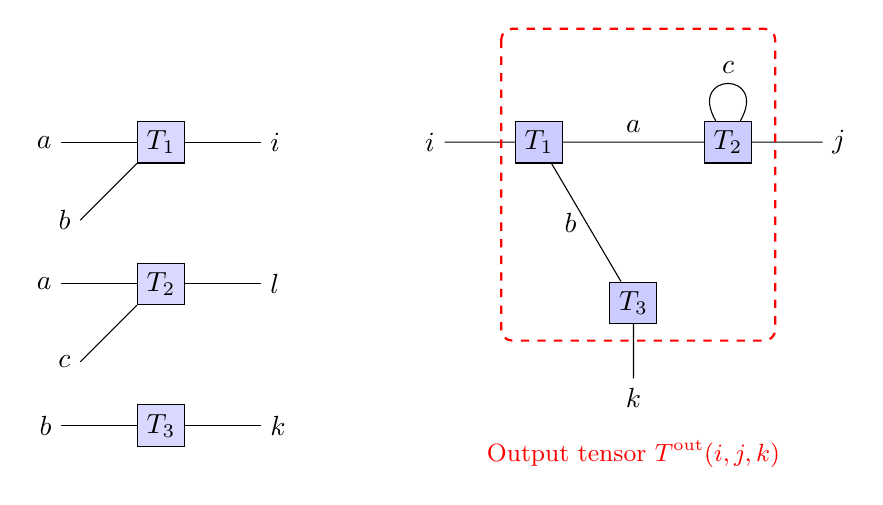
\begin{tikzpicture}[scale=1.2, every node/.style={scale=1.0}]

  % ==== Left: Tensor definitions ====

  % g1
  \node[draw, rectangle, fill=blue!15] (tg1) at (0,3) {$T_1$};
  \draw[-] (tg1.west) -- +(-0.8,0) node[left] {$a$};
  \draw[-] (tg1.south west) -- +(-0.6,-0.6) node[left] {$b$};
  \draw[-] (tg1.east) -- +(0.8,0) node[right] {$i$};

  % g2
  \node[draw, rectangle, fill=blue!15] (tg2) at (0,1.5) {$T_2$};
  \draw[-] (tg2.west) -- +(-0.8,0) node[left] {$a$};
  \draw[-] (tg2.south west) -- +(-0.6,-0.6) node[left] {$c$};
  \draw[-] (tg2.east) -- +(0.8,0) node[right] {$l$};

  % g3
  \node[draw, rectangle, fill=blue!15] (tg3) at (0,0) {$T_3$};
  \draw[-] (tg3.west) -- +(-0.8,0) node[left] {$b$};
  \draw[-] (tg3.east) -- +(0.8,0) node[right] {$k$};

  % ==== Right: Tensor network ====

  % Nodes
  \node[draw, rectangle, fill=blue!20] (g1) at (4,3) {$T_1$};
  \node[draw, rectangle, fill=blue!20] (g2) at (6,3) {$T_2$};
  \node[draw, rectangle, fill=blue!20] (g3) at (5,1.3) {$T_3$};

  % External indices
  \draw[-] (g1) -- +(-1,0) node[left] {$i$};
  \draw[-] (g2) -- +(1,0) node[right] {$j$};
  \draw[-] (g3) -- +(0,-0.8) node[below] {$k$};

  % Internal contractions
  \draw[-] (g1) -- (g2) node[midway, above] {$a$};
  \draw[-] (g1) -- (g3) node[midway, left] {$b$};

  % self-loop for g2
  \draw (g2) to[out=120,in=60,looseness=6] node[above] {$c$} (g2);

  % Box around the whole tensor network to indicate output f(i,j,k)
 \draw[rounded corners, thick, dashed, red] ($(g1) + (-0.4,1.2)$) rectangle ($(g3) + (1.5,-0.4)$);
\node[red] at ($(g3) + (0,-1.6)$) {\small Output tensor $T^{\rm out} (i,j,k)$};
\end{tikzpicture}
\caption{
Left panel: visual representations of the component tensors $T_1, T_2, T_3$;  
Right panel: visualization of the function 
$T^{\rm out} (i,j,k) = \sum_{a,b,c} T_1 (a,b,i) T_2 (a,c,j) T_3 (b,k)$ using the tensor network graphical language.
}
\label{fig:tensor_network_example}
\end{figure}
\fi

\begin{remark}
\label{rem:Python}
The \Einsum{} operation has been implemented in highly optimized Python libraries such as \numpyeinsum{} and \torcheinsum{}. These efficient algorithmic subroutines, enabling efficient \Einsum{} operation in practice, serve as the building blocks of our algorithm. Notably, developed for training large overparameterized neural networks in tensor forms, \torcheinsum{} is also designed to leverage GPU computing to further enhance the scalability and speed of the \Einsum{} operation, as we will demonstrate using an example from statistics in Section~\ref{sec:example_hoif}.
\end{remark}

\begin{remark}
\label{rem:tensor networks}
The \Einsum{} operation is frequently employed in scientific computing problems. For example, the \Einsum{} operation serves as a basic algorithmic subroutine for computation over tensor (hyper)networks, a useful mathematical language adopted by the quantum computing and quantum information community \citep{markov2008simulating}. % The tensor network formulation can help visualize summations (partial traces) over tensors in the language of graphs (e.g. Figure~\ref{fig:tensor_network_example} visualizing Example~\ref{eg:tensor}). 
Although we do not directly adopt the tensor network formulation, our strategy is quite similar in that we also establish a correspondence between the \Einsum{} operation and operations on graphs -- see Section~\ref{sec:alg_v} for more details. 
\end{remark}

% Tensor contraction (generalizing the classical Einstein summation/Einsum) serves as a foundational computational primitive in our proposed algorithm for efficiently and exactly computing $U$/$V$-statistics. 

\iffalse

Tensor networks are well-established tools in quantum information and quantum computing \citep{stoudenmire2018learning}, offering a structured and visual representation of tensors with decomposable structures. For instance, the following rank-3 tensor $f (i, j, k)$ is decomposed into three component tensors, with internal indices $ a, b, c $ that are independently summed over. These internal indices are referred to as \emph{contracted indices}, in contrast to the \emph{free indices} $ i, j, k $, which determine the structure of the output tensor:
\begin{equation*}
    f(i, j, k) = \sum_{a,b,c} g_1(a, b, i)\, g_2(a, c, j)\, g_3(b, k).
\end{equation*}

\Chen{Will update and polish later, maybe one example contain all conception, now example lack  multiple edges and hyper edges. Below will coantain all conception.
\begin{equation*}
    f(i, j, k) = \sum_{a,b,c,d} g_1(a, b, d, i)\, g_2(a, b, c, j)\, g_3(a, b, c) g_4(b,c,k).
\end{equation*}
}
This process can be represented as a tensor network, however, unlike a simple graph, it may include self-loops (representing internal contractions within a single tensor), multiple edges (representing repeated shared indices between tensors), and dangling edges (corresponding to free indices that are not contracted), as shown in Figure~\ref{fig:tensor_network_example}, where each tensor corresponds to a vertex and each edge represents an index. Edges shared between nodes correspond to contracted indices that appear in multiple tensors and are summed over. A self-loop on a vertex indicates a contracted index that appears only within that tensor. Computing $ f(i, j, k) $ from the tensors $ g_1, g_2, g_3 $ via summation over all contracted indices is termed as \emph{tensor contraction}.

\Lin{I think we can keep this figure in the main text and use it to illustrate einsum. we say it is adopted from the tensor network literature and then expand upon in the appendix.}

\Lin{let's do another real tensor example here.}

\begin{remark}
\label{rem:libraries}
Several open-source libraries offer highly optimized implementations of the \Einsum{} operation, including \numpyeinsum{} from \numpy{} and \torcheinsum{} from \torch{}. These efficient algorithmic routines, enabling efficient \Einsum{} operation in practice, serve as the building blocks for our algorithm. Notably, developed for training large overparameterized neural networks in tensor forms, \torch{} is designed to leverage GPU computing to further substantially enhance the scalability and speed of the \Einsum{} operation, as we will demonstrate in Section~\ref{sec:examples} via three concrete examples from statistics.
\end{remark}
\fi



\iffalse
\begin{example}
\label{example:einsum_jin}
In \citet{jin2025counting}, \Lin{for what purpose?} the authors decompose an $8$-th order $U$-statistic into 44 terms, as detailed in their Table~1. Among them, 43 terms can be expressed using standard matrix operations such as matrix multiplication, Hadamard product, and transposition. However, there is one term that cannot be represented in terms of standard matrix operations. This difficulty motivates the authors of \citet{jin2025counting} to develop and adopt an LLM-assisted customized programming approach to handle such terms \Lin{maybe we should be a bit more specific}. This term reads as:
\begin{equation}
\label{full-sum}
C = \sum_{\bar{i}_{4} \in [n]^4} (A \circ A)_{i_1, i_2} A_{i_1, i_3} A_{i_1, i_4} A_{i_2, i_3} A_{i_2, i_4} (A \circ A)_{i_3, i_4},
\end{equation}
where $A \in \mathbb{R}^{n \times n}$ and $A \circ A$ is the Hadamard product. Interestingly, adopting the framework in our paper, \eqref{full-sum} can be directly computed using \Einsum{}:
\begin{equation*}
C \equiv \tensorcontraction ((\underbrace{A,
\dots, A}_{\textrm{8 times}}), \; ((1,2),(1,2),(1,3),(1,4),(2,3),(2,4),(3,4),(3,4))),
\end{equation*}
which can be directly computed using the algorithm to be shown later in our paper.
\end{example}
\fi

\subsection{Useful Concepts from Graph Theory}
\label{sec:graph}

\iffalse
\begin{definition}[Partition]\label{def:partition}
    Let $S$ be a non-empty set, $\sPi$ a collection of non-empty subsets of $S$. $\sPi$ is a partition of $S$, if
    \begin{itemize}
        \item $A \cap B = \emptyset, \quad \forall A, B \in \sPi: A \neq B$, 
        \item $\cup_{B \in \sPi} B = S$. 
    \end{itemize}

    All partitions of set $S$ is denoted by $\partitionp{S}$. If $S = [m]$ for positive integer $m$, it is denoted by $\partitionp{m}$. 
\end{definition}

\begin{definition}[Permutation]\label{def:permutation}
    Let $S$ be a non-empty set with cardinality $m$. A permutation of $S$ is an $m$-tuple whose elements in different indices is different to each other. 
\end{definition}
\fi

In this section, we recall three key concepts from graph theory that are central 
to our complexity-theoretic characterization. We follow the terminology of 
\citet{bodlaender2010treewidth} for \emph{vertex elimination} and \emph{treewidth}, 
which captures the dominant computational complexity of our problem. 
We also recall the notion of \emph{quotient graph}, adopted from 
\citet{sanders2012high}, which underlies the decomposition of a $U$-statistic 
into a linear combination of $V$-statistics.

\begin{definition}[Vertex Elimination]
\label{def:vertex_elimination}
Let $G = (V, E)$ be a graph and $v \in V$. We define the operation of eliminating $v$ from $V$ as first connecting $\neighborvg{v}{G}$ (the neighbor of $v$ w.r.t. $G$) by edges to form a clique and then removing the vertex $v$ and all edges incident to $v$. The resulting graph is denoted by $\eliminatevg{v}{G}$. 
\end{definition}

\begin{definition}[Treewidth]
\label{def:treewidth_elimination}
Let $G = (V, E)$ be a graph with $|V| = n$. For $\sigma \in \perm{V}$, $(G_i^{\sigma})_{i=1}^n$ is a sequence of graphs recursively defined as $G_i^\sigma = \eliminatevg{\sigma[i]}{G_{i-1}^\sigma}$ with $G_0^\sigma = G$. Then the treewidth of the graph $G$ is defined as 
\begin{equation*}
\treewidthp{G} \coloneqq \min_{\sigma \in \perm{V}} \max_{i \in [n]} \degp{\sper[i]}{G_{i-1}^\sigma}. 
\end{equation*}
\end{definition}

% \Chen{ Quotient Graph is a well studied concept (GPT has told me, also wiki and lots of paper titles, but the concept of Quotient Graph Family defined below seems no one can cite), it describes when we let "1=2","3=4" will corresponding to what operation between the graph ( specially, only merging two indies called Vertex-Identification we used to want to use ), the family of all quotient graph is the family of all graph corresponding to all "$V$-statistics" split from the $U$-statistics.  }
\begin{definition}[Quotient Graph]
\label{def:quotient_graph}
Let $G = (V, E)$ be a graph. A quotient graph associated with $G$ w.r.t. a partition $\sPi$ of $V$ is defined as $G/\pi \coloneqq (\pi, E_{\pi})$, where
\begin{equation*}
    E_\pi = \left\{\{B_i,B_j\} \subseteq \pi \mid \exists \, v_1 \in B_i, v_2 \in B_j, \text{ such that } \{v_1, v_2\} \in E\right\}. 
\end{equation*}
\end{definition}


\section{A New Algorithm of Computing \pdfu{}-Statistics}
\label{sec:alg_u_v}

We are ready to present our new algorithm for exactly computing $U$-statistics, along with an analysis of the time complexity. Our algorithm has been implemented in an open source Python package \package{} (and its \href{https://github.com/cxy0714/U-Statistics-R}{R} interface). We begin by introducing the \emph{multiplicative-decomposable} (MD) structure of the $U$/$V$-statistic kernel in Section~\ref{sec:decomposition}, followed by the new algorithm and complexity analysis for $V$- and $U$-statistics in Section~\ref{sec:alg_v} and Section~\ref{sec:alg_u}.

% Throughout this section, we will use a running example related to Example~\ref{eg:running} to delineate our proposed algorithm and certain theoretical results.

\subsection{The Multiplicative-Decomposable Kernels}
\label{sec:decomposition}

The \emph{multiplicative-decomposable} (MD) structure is the key assumption we impose on the kernel of the $U$-statistic to be computed. This structure is essential for developing more efficient algorithms for exactly computing $U$/$V$-statistics than trivially summing over all $m$-out-of-$n$ permutations/$[n]^{m}$. Similar concepts are commonly used to develop numerical algorithms for solving partial differential equations.

\begin{definition}[Multiplicative Decomposition]\label{def:mul_decomp}
Let $\samplespace$ be a non-empty set, $m$ a positive integer, and $h: \samplespace^m \to \bbR$. Suppose $\calA \coloneqq (A_k)_{k=1}^K \in [m]^{**}$ satisfies $\bigcup_{k=1}^K \takesetp{A_k} = [m]$, and let $\calH \coloneqq (h_k)_{k=1}^K$ be a tuple of functions where each $h_k$ is defined on $\samplespace^{|A_k|}$. $\calH \times \calA$, consisting of ordered pairs of the form $(h_{k}, A_{k})$ for $k \in [K]$, is called a multiplicative decomposition of the function $h$, if for any $\bm{x} \in \samplespace^m$, 
\begin{align*}
h(\bm{x}) = \prod_{k=1}^K h_k\big(\bm{x}[A_k]\big).
\end{align*}
\end{definition}
In the sequel, we refer to the function tuple $\calH$ as the kernel components and the index tuple $\calA$ as the decomposition signature. For convenience, we say that a kernel $h$ allows a (non-trivial) MD structure $\calH \times \calA$ if $K > 1$. $U$-statistic kernels with MD structures are common in statistics. We will provide three examples in Section~\ref{sec:examples} and Appendix~\ref{app:examples}.

To utilize the \Einsum{} operation to compute $U$/$V$-statistics, we need to store pieces of the underlying statistics in tensor format. We term this step as \emph{tensorization}. Let $h$ be the kernel of some $U$/$V$-statistic permitting a MD structure $\calH \times \calA$, where $\calH \coloneqq (h_k)_{k=1}^K$ and $\calA \coloneqq (A_k)^K_{k=1}$. Given a sample $\bm{X} \in \samplespace^n$, the tensorization step constructs a tuple of tensors $\calT \coloneqq (T_k)_{k=1}^K$ as follows:
\begin{align*}
T_k (\alpha_k) = h_k (\bm{X}[\alpha_k]), \quad \forall \, \alpha_k \in [n]^{|A_k|}, \, \forall \, k \in [K].
\end{align*}
Then following Definition~\ref{def:v_stat} and Definition~\ref{def:mul_decomp},
\begin{align}\label{eq:tensorization_v}
\vstat(h, \bm{X}) = \sum_{\alpha \in [n]^m} h(\bm{X}[\alpha]) \equiv \sum_{\alpha \in [n]^m} \prod_{k=1}^K h_k(\bm{X}[\alpha[A_k]]) \equiv \sum_{\alpha \in [n]^m} \prod_{k=1}^K T_k(\alpha[A_k]), 
\end{align}
which implies that the $V$-statistic $\vstat(h, \bm{X})$ can be equivalently expressed by using the tuple of tensors $\calT$ and the decomposition signature $\calA$. As will be seen in Section~\ref{sec:alg_u}, we can also use $\calT$ and $\calA$ to represent $U$-statistics. Hence $\vstat(h, \bm{X})$ and $\ustat(h, \bm{X})$ can be equivalently denoted as $\ustat(\calT, \calA)$ and $\vstat(\calT, \calA)$, respectively. We summarize the tensorization step in Algorithm~\ref{alg:tensorization} below, which constitutes the first step of our new algorithm for exactly computing a $V$-statistic.

\begin{algorithm}
    \caption{Tensorization of Kernel Function}
    \label{alg:tensorization}
    \begin{algorithmic}[1]
        \Require 
            \Statex A kernel $h$ with decomposition components $\calH \coloneqq (h_k: \bbX^{m_k} \to \reals)_{k=1}^K$
            \Statex A sample $\bm{X} = (X_1, \dots, X_n) \in \samplespace^n$ from a non-empty set $\samplespace$
        \Ensure A tuple of tensors $\calT \coloneqq (T_k: [n]^{m_k} \to \reals)_{k=1}^K$, where $T_k$ is the tensorized $h_k$

        \Function{Tensorization}{$\calH, \bm{X}$}
            \For{$k \in [K]$}  
                \Comment{Iterate over each factor of kernel $h$}
                \For{$\alpha \in [n]^{m_k}$}  
                    \Comment{Iterate over all $m_k$-dimensional indices}
                    \State $T_k(\alpha) \gets h_k(\bm{X}[\alpha])$  
                    \Comment{Evaluate $h_k$ on $\bm{X} [\alpha]$}
                \EndFor
            \EndFor
            \State \Return $\calT \coloneqq (T_k)_{k=1}^K$  
        \EndFunction
    \end{algorithmic}
\end{algorithm}

% The above procedure, referred to as the tensorization of a $V$-statistic, constitutes a data processing step that evaluates the kernel function on the sample list using its factorized components, as presented in Algorithm~\ref{alg:tensorization} in a for-loop manner. The computational complexity of this preprocessing step varies significantly across different cases. Therefore, we do not attempt to analyze it in detail. Instead, our focus lies in characterizing the complexity of computing the final value once all tensors have been prepared.

The MD structure plays an essential role in reducing the complexity of exactly computing $V$-statistics. % This step is necessary even if the result does not need to stored via tensor \Lin{I do not understand; we could've do for loop without storing any tensor by just accessing to the kernel and the data matrix...}. \Zhang{For loop case, each time we evaluate kernel on one tuple of arguments and sum to result. The evaluations just distribute in steps of loop and aren't stored as tensor. But they still exist and are of computational cost. }
Without a (nontrivial) MD structure, the time complexity of computing an $m$-th order $V$-statistic is generally $\less (n^m)$ as we need to evaluate a function of $m$ arguments on all tuples of $[n]^m$. But if a particular MD structure holds, the time complexity may scale with $\less (n^{m_{\mathrm{max}}})$ where $m_{\mathrm{max}} \coloneqq \max_{k \in [K]} |A_k|$ since we just need to evaluate each  $h_k$ on all tuples of $[n]^{|A_k|}$ for $k \in [K]$. As $m_{\mathrm{max}}$ can be smaller than $m$, it is possible to improve the time complexity dramatically in practice. More details on the complexity analysis and intuition can be found in Section~\ref{sec:alg_v} below.

\setcounter{example}{1}
\begin{subexample}
\label{eg:running-a}
Recalling Example~\ref{eg:running}. The \Einsum{} operation can be seen as a $V$-statistic whose kernel function $h$ has a MD structure $\calH \times \calA$ with $\calH = (h_1, h_2, h_3)$, signature $\calA = ( (1,2),(2,3),(3,4))$ and $n$ sample points $\bm{X} \in \samplespace^{n}$. Tensorization of $\calH$ outputs tensors $\calT = ( T_1, T_2, T_3)$ such that:
\begin{equation*}
T_i (j,k) = h_i (\bm{X}_{j}, \bm{X}_{k}),  \, (j,k) \in [n]^2,  \, i = 1,2,3.
\end{equation*}
The $V$-statistic and $U$-statistic with kernel $h$ are respectively:
\begin{align*}
\vstat(h, \bm{X}) = \vstat (\calT, \calA) = \Einsum{}(\calT, \calA), \quad \ustat(h, \bm{X}) = \ustat(\calT, \calA).
\end{align*}
% See Figure~\ref{fig:flow} for a visual illustration.
\end{subexample}



\iffalse
We now consider an example of $V$-statistic. Suppose that the kernel function $h: \bbX^{4} \rightarrow \bbR$ can be decomposed as $h (x_1, x_2, x_3, x_4) = h_1 (x_1, x_2, x_3) h_2 (x_3, x_4)$ so $\calH = (h_1, h_2)$ and $\calA = (A_1, A_2)$ with $A_1 = (1, 2, 3)$ and $A_2 = (3, 4)$, and we are interested in computing the following $V$-statistic with kernel $h$:
\begin{align*}
\mathbb{V} (h, \bm{X}) & = \sum_{\alpha \in [n]^{4}} h (\bm{X} [\alpha]) \\
& = \sum_{\alpha \in [n]^{4}} h_1 (\bm{X} [\alpha [1, 2, 3]]) h_2 (\bm{X} [\alpha [3, 4]]) \\
& = \sum_{\alpha \in [n]^{4}} T_1 (\alpha [1, 2, 3]) T_2 (\alpha [3, 4])
\end{align*}
where in the last line we apply the tensorization algorithm (Algorithm~\ref{alg:tensorization}) to $\calH$ to obtain the tensor tuple $\calT = (T_1, T_2)$.
\fi



\subsection{The Algorithm of Computing \pdfv{}-Statistics}
\label{sec:alg_v}

In this section, we show that $V$-statistics can be computed via the \Einsum{} operation. Let $\vstat(h, \bm{X})$ be an $m$-th order $V$-statistic with kernel $h$ and sample $\bm{X}$ of size $n$. Suppose that the kernel $h$ satisfies MD structure $(\calH \coloneqq (h_k)_{k=1}^K) \times (\calA \coloneqq (A_k)_{k=1}^K)$. As we have seen, $\vstat(h, \bm{X})$ has an equivalent tensorized form $\vstat(\calT, \calA)$, where $\calT$ is the output of Algorithm~\ref{alg:tensorization}. 

By definition, $\calA$ constitutes an \Einsum{} notation and $\calT$ can be represented by $\calA$ (see Definition~\ref{def:tensor_contraction}), then we have
\begin{equation*}
    \tensorcontraction(\calT, \calA) = \sum_{\alpha \in [n]^m} \prod_{k=1}^K T_k(\alpha[A_k]). 
\end{equation*}
Comparing the above equation with \eqref{eq:tensorization_v}, we immediately have 
\begin{align*}
    \vstat(h, \bm{X}) = \tensorcontraction(\calT, \calA), 
\end{align*}
i.e. computing a $V$-statistic is the same as performing an \Einsum{} operation. Algorithm~\ref{alg:v_stats} describes how $V$-statistics can be computed by the \Einsum{} operation.

\begin{algorithm}
    \caption{Tensorization Algorithm of $V$-Statistics}
    \label{alg:v_stats}
    \begin{algorithmic}[1]
        \Require 
            \Statex A kernel function $h: \samplespace^m \to \reals$ permitting a MD structure $\calH \times \calA$
            \Statex A sample $\bm{X} \in \samplespace^n$ from a non-empty set $\samplespace$
        \Ensure $V$-statistic $\vstat(h, \bm{X})$

        \Function{Vstats}{$\calH, \calA; \bm{X}$}
            \State $\calT \gets$ \Call{Tensorization}{$\calH, \bm{X}$}
            \Comment{see Algorithm~\ref{alg:tensorization}}
            \State $v \gets \tensorcontraction(\calT, \calA)$\footnotemark 
            % (with the \Einsum{} ordering found using \opteinsum{}) 
            \State \Return $v$
        \EndFunction
    \end{algorithmic}
\end{algorithm}
\footnotetext{\label{fn:einsum}In our implementation of \package{}, we directly call \numpyeinsum{} or \torcheinsum{}, with the summation ordering optimized by \opteinsum{}. }
The time complexity of computing a $V$-statistic can obviously be characterized by that of the \Einsum{} operation. The essential idea is to establish a correspondence between the \Einsum{} operation and the vertex elimination operation (Definition~\ref{def:vertex_elimination}) over a graph associated with the \Einsum{} notation. The time complexity can in turn be characterized by the treewidth (Definition~\ref{def:treewidth_elimination}) of that graph. Similar idea has also been exploited in \citet{markov2008simulating}, in which the time complexity of tensor contraction (a special case of the \Einsum{} operation) is characterized by the treewidth of the underlying tensor network. 

To facilitate presentation, we first introduce the notion of ``decomposition graph'' associated with a given \Einsum{} notation, which captures all the information needed to establish the time complexity of computing a particular $V$-statistic.

\begin{definition}[Decomposition Graph]\label{def:graph_decomp}
Let $\calA$ be an \Einsum{} notation with no output. The decomposition graph associated with $\calA$ (or equivalently the decomposition signature $\calA$) is a graph $\graphform{\calA} = (V_{\calA}, E_{\calA})$ where
    \begin{itemize}
        \item $V_{\calA} = \indexset(\calA)$, 
        \item $E_{\calA} = \big\{ \{i, j\} \subseteq V_{\calA} \mid \exists \, A \in \calA; \text{ such that } i, j \in \takesetp{A} \big\}$.
    \end{itemize}
\end{definition}

% \begin{remark}
% The decomposition graph is, in fact, a line graph commonly used in the tensor (hyper)network literature, where tensors are represented as vertices and indices as edges \Lin{common indices between tensors?}. \Lin{unclear English} However, in this paper, we do not directly adopt the tensor network graph; the rationale for this choice will be provided in Remark~?. \Lin{don't quite understand the previous sentence} In \citet{markov2008simulating}, the authors established a connection between the treewidth of the decomposition graph defined here and the dominating terms in the computational complexity of the corresponding tensor network contraction. This relationship will be discussed in detail in Section~\ref{sec:alg_v}, where we characterize the complexity of computing $V$-statistics.
% \end{remark}

% \Lin{we should use the examples earlier as well.}

We use several concrete examples to illustrate the above definition.

\begin{example}[\Einsum{} notations and its decomposition graphs]
Figure~\ref{fig:graphs_examples} below illustrates several examples of decomposition graphs associated with different decomposition signatures. The underlying idea is to treat each index in $\calA$ as a vertex and to add an edge between two vertices whenever the corresponding indices co-occur in the same tuple. Repeated tuples do not create multiple edges (see Figures~\ref{fig:graph_hoif_4_2} and~\ref{fig:graph_hoif_4_5}). Moreover, different decomposition signatures can yield the same decomposition graph (see Figures~\ref{fig:graph_motif_4} and~\ref{fig:graph_same_motif_4}).
\begin{figure}[htbp]
\centering
% First row
\begin{subfigure}{0.22\textwidth}
\centering
 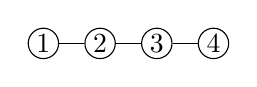
\begin{tikzpicture}[scale=0.6, baseline={(0,-0.2)}]
    \node[draw, circle, inner sep=1pt] (1) at (0,0) {1};
    \node[draw, circle, inner sep=1pt] (2) at (1.2,0) {2};
    \node[draw, circle, inner sep=1pt] (3) at (2.4,0) {3};
    \node[draw, circle, inner sep=1pt] (4) at (3.6,0) {4};
    \draw (1) -- (2) -- (3) -- (4);
\end{tikzpicture} 
\caption{$\calA = ((1,2),(2,3),(3,4))$}
\label{fig:graph_hoif_4_1}
\end{subfigure}
\hfill
\begin{subfigure}{0.22\textwidth}
\centering
 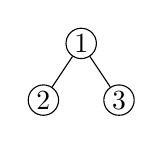
\begin{tikzpicture}[scale=0.6, baseline={(0,-0.2)}]
    \node[draw, circle, inner sep=1pt] (1) at (0,0.6) {1};
    \node[draw, circle, inner sep=1pt] (2) at (-0.8,-0.6) {2};
    \node[draw, circle, inner sep=1pt] (3) at (0.8,-0.6) {3};
    \draw (1) -- (2);
    \draw (1) -- (3);
\end{tikzpicture} 
\caption{$\calA = ((1,2), (2,1), (1,3))$}
\label{fig:graph_hoif_4_2}
\end{subfigure}
\hfill
\begin{subfigure}{0.22\textwidth}
\centering
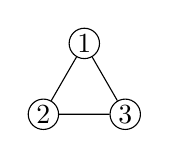
\begin{tikzpicture}[scale=0.6, baseline={(0,-0.2)}]
    \node[draw, circle, inner sep=1pt] (1) at (90:1) {1};
    \node[draw, circle, inner sep=1pt] (2) at (210:1) {2};
    \node[draw, circle, inner sep=1pt] (3) at (330:1) {3};
    \draw (1) -- (2) -- (3) -- (1);
\end{tikzpicture} 
\caption{$\calA = ((1,2), (2,3), (3,1))$}
\label{fig:graph_hoif_4_3_motif_3}
\end{subfigure}
\hfill
\begin{subfigure}{0.22\textwidth}
\centering
 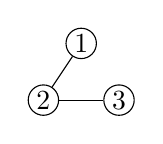
\begin{tikzpicture}[scale=0.6, baseline={(0,-0.2)}]
    \node[draw, circle, inner sep=1pt] (1) at (0,0.6) {1};
    \node[draw, circle, inner sep=1pt] (2) at (-0.8,-0.6) {2};
    \node[draw, circle, inner sep=1pt] (3) at (0.8,-0.6) {3};
    \draw (1) -- (2);
    \draw (2) -- (3);
\end{tikzpicture} 
\caption{$\calA = ((1,2), (2,3), (3,2))$}
\label{fig:graph_hoif_4_4}
\end{subfigure}

\vspace{0.5cm}

% Second row
\begin{subfigure}{0.22\textwidth}
\centering
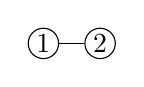
\begin{tikzpicture}[scale=0.6, baseline={(0,-0.2)}]
    \node[draw, circle, inner sep=1pt] (1) at (0,0) {1};
    \node[draw, circle, inner sep=1pt] (2) at (1.2,0) {2};
    \draw (1) -- (2);
\end{tikzpicture} 
\caption{
$\calA = ((1,2), (2,1), (1,2))$}
\label{fig:graph_hoif_4_5}
\end{subfigure}
\hfill
\begin{subfigure}{0.22\textwidth}
\centering
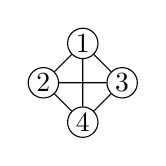
\begin{tikzpicture}[scale=0.5, baseline={(0,-0.2)}]
    \node[draw, circle, inner sep=1pt] (1) at (0,1) {1};
    \node[draw, circle, inner sep=1pt] (2) at (-1,0) {2};
    \node[draw, circle, inner sep=1pt] (3) at (1,0) {3};
    \node[draw, circle, inner sep=1pt] (4) at (0,-1) {4};
    \draw (1) -- (2) -- (3) -- (4) -- (1);
    \draw (1) -- (3);
    \draw (2) -- (4);
\end{tikzpicture}
\caption{
$\calA = ((1,2),(1,3),(1,4),$ \\
$(2,3),(2,4),(3,4))$}
\label{fig:graph_motif_4}
\end{subfigure}
\hfill
\begin{subfigure}{0.22\textwidth}
\centering
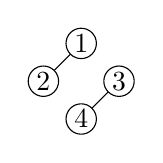
\begin{tikzpicture}[scale=0.6, baseline={(0,-0.2)}]
    \node[draw, circle, inner sep=1pt] (1) at (0,0.8) {1};
    \node[draw, circle, inner sep=1pt] (2) at (-0.8,0) {2};
    \node[draw, circle, inner sep=1pt] (3) at (0.8,0) {3};
    \node[draw, circle, inner sep=1pt] (4) at (0,-0.8) {4};
    \draw (1) -- (2) ;
    \draw (3) -- (4) ; 
\end{tikzpicture}
\caption{$\calA = ((1,2),(3,4))$}
\label{fig:graph_dcov_1}
\end{subfigure}
\hfill
\begin{subfigure}{0.22\textwidth}
\centering
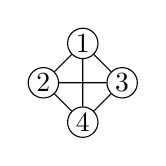
\begin{tikzpicture}[scale=0.5, baseline={(0,-0.2)}]
    \node[draw, circle, inner sep=1pt] (1) at (0,1) {1};
    \node[draw, circle, inner sep=1pt] (2) at (-1,0) {2};
    \node[draw, circle, inner sep=1pt] (3) at (1,0) {3};
    \node[draw, circle, inner sep=1pt] (4) at (0,-1) {4};
    \draw (1) -- (2) -- (3) -- (4) -- (1);
    \draw (1) -- (3);
    \draw (2) -- (4);
\end{tikzpicture}
\caption{ $\calA = ((1,2,3),(1,3,4),$ \\
$(1,2,4),(2,3,4))$}
\label{fig:graph_same_motif_4}
\end{subfigure}
\caption{Examples of decomposition graphs of different decomposition signatures.}
\label{fig:graphs_examples}
\end{figure}
\end{example}

We are ready to present the following ``optimistic'' estimate of the time complexity of the \Einsum{} operation. The proof of the proposition below is deferred to Appendix~\ref{app:complexity_einsum}.

\begin{proposition}
\label{pro:complexity_einsum}
Let $\calA$ be an \Einsum{} notation with no output, and $G_\calA$ be the corresponding decomposition graph of $\calA$. Then there exists an algorithm with a particular \Einsum{} ordering such that for any set of tensors $\calT$ that can be represented by the \Einsum{} notation $\calA$, the time complexity of $\tensorcontraction(\calT, \calA)$ is $\less(|\calA|n^{\treewidthp{G_\calA}+1})$. 
\end{proposition}
 
\iffalse
Figure~\ref{fig:flow} exhibits the process of deriving the runtime complexity for the $V$-statistic in Example~\ref{eg:running-a} to serve as a simple illustration.

\begin{figure}[htbp]
\centering
\begin{tikzpicture}[
    node distance=1.7cm and 1.6cm,
    every node/.style={font=\small},
    expr/.style={draw, rectangle, rounded corners, align=center, text width=5.5cm, minimum height=1.5cm},
    decomp/.style={draw, rectangle, align=center, text width=3.1cm, minimum height=1.2cm},
    arrow/.style={-{Latex}, thick},
    point/.style={circle, draw, minimum size=5.5mm, inner sep=0pt, font=\small},
    graphbox/.style={draw, align=center, minimum width=1.8cm, minimum height=1.2cm, inner sep=3pt}
]
% === COLUMN 1: Tensor expressions ===
\node[expr] (e1) {
    $\displaystyle \sum_{ {\color{red}i_1}, i_2, i_3, i_4} h_1({\color{red}i_1}, i_2)\, h_2(i_2, i_3)\, h_3(i_3, i_4)$
};
\node[expr, below=of e1] (e2) {
    $\displaystyle \sum_{{\color{blue}i_2}, i_3, i_4} h_4({\color{blue}i_2})\, h_2({\color{blue}i_2}, i_3)\, h_3(i_3, i_4)$
};
\node[expr, below=of e2] (e3) {
    $\displaystyle \sum_{ {\color{orange}i_3}, i_4} h_5({\color{orange}i_3})\, h_3({\color{orange}i_3}, i_4)$
};
\node[expr, below=of e3] (e4) {
    $\displaystyle \sum_{{\color{violet}i_4}} h_6({\color{violet}i_4})$
};
\node[expr, below=of e4] (e5) {
    End \\
    Max complexity $O(n^2)$
};

% === COLUMN 2: Function Decompositions ===
\node[decomp, right=of e1] (d1) {
    $((1,2)(2,3)(3,4))$
};
\node[decomp, below=of d1] (d2) {
    $((2)(2,3)(3,4))$
};
\node[decomp, below=of d2] (d3) {
    $((3)(3,4))$
};
\node[decomp, below=of d3] (d4) {
    $((4))$
};
\node[decomp, below=of d4] (d5) {
    End
};

% === COLUMN 3: Graphs ===
\node[graphbox, right=of d1] (g1) {
    \begin{tikzpicture}[scale=0.9]
        \node[point, fill=red!20] (1) at (0, 0.7) {\textcolor{red}{$1$}};
        \node[point] (2) at (1, 0.7) {$2$};
        \node[point] (3) at (2, 0.7) {$3$};
        \node[point] (4) at (3, 0.7) {$4$};
        \draw[red, thick] (1) -- (2);
        \draw (2) -- (3) -- (4);
    \end{tikzpicture}
};
\node[graphbox, below=of g1] (g2) {
    \begin{tikzpicture}[scale=0.9]
        \node[point, fill=blue!20] (2) at (0, 0.7) {\textcolor{blue}{2}};
        \node[point] (3) at (1, 0.7) {3};
        \node[point] (4) at (2, 0.7) {4};
        \draw[blue, thick] (2) -- (3);
        \draw (3) -- (4);
    \end{tikzpicture}
};
\node[graphbox, below=of g2] (g3) {
    \begin{tikzpicture}[scale=0.9]
        \node[point, fill=orange!30] (3) at (0, 0.7) {\textcolor{orange}{3}};
        \node[point] (4) at (1, 0.7) {4};
        \draw[orange, thick] (3) -- (4);
    \end{tikzpicture}
};
\node[graphbox, below=of g3] (g4) {
    \begin{tikzpicture}[scale=0.9]
        \node[point, fill=violet!30] (4) at (0, 0.7) {\textcolor{violet}{4}};
    \end{tikzpicture}
};
\node[graphbox, below=of g4] (g5) {
    End \\
    $\treewidthp{G} = \max_{1\le i \le 4} \deg_{i} = 1$
};

% === Arrows: Computation steps ===
\draw[arrow] (e1) -- node[left, align=left] {
    Sum over $\color{red}i_1$ \\
    $h_4(i_2) = \sum_{\color{red}i_1} h_1$
} (e2);

\draw[arrow] (e2) -- node[left, align=left] {
    Sum over $\color{blue}i_2$ \\
    $h_5(i_3, i_4) = \sum_{\color{blue}i_2} h_4 h_2$
} (e3);

\draw[arrow] (e3) -- node[left, align=left] {
    Sum over $\color{orange}i_3$ \\
    $h_6(i_4) = \sum_{\color{orange}i_3} h_5 h_3$
} (e4);

\draw[arrow] (e4) -- node[left, align=left] {
    Sum over $\textcolor{violet}{i_4}$ \\
    Scalar = $\sum h_6$
} (e5);

% === Arrows: Decomposition steps ===
\draw[arrow] (d1) -- (d2);
\draw[arrow] (d2) -- (d3);
\draw[arrow] (d3) -- (d4);
\draw[arrow] (d4) -- (d5);

% === Arrows: Graph evolution ===
\draw[arrow] (g1) -- node[right, align=left] {
    Eliminate $\color{red}1$ \\
    $\deg_1 =1$
} (g2);
\draw[arrow] (g2) -- node[right, align=left] {
    Eliminate $\color{blue}2$ \\
    $\deg_2 =1$
} (g3);
\draw[arrow] (g3) -- node[right, align=left] {
    Eliminate $\color{orange}3$ \\
    $\deg_3 =1$
} (g4);
\draw[arrow] (g4) -- node[right, align=left] {
    Eliminate $\textcolor{violet}{4}$ \\
    $\deg_4=0$
} (g5);
\end{tikzpicture}
\caption{Visualizing the derivation of the time-complexity for the running example.}
\label{fig:flow}
\end{figure}
\fi

\iffalse
\Lin{I personally find the remark below is sufficiently clear without the need of going into the rabbit hole of tensor-wise or index-wise stuff.}

\Zhang{This should be discussed. There are 2 gaps: heuristic and optimal; tensor-wise (or pair-wise) and index-wise}

\Chen{
Remark 1 can say index-wise manner optimal ordering is NP-hard

Remark 2 can say index-wise ordering can always represented by tensor-wise ordering which now used in pacakage, but in paractice, still a gap between two manner, can be shown in Sec~4.3
}
\fi

\begin{remark}[\Einsum{} summation ordering in practice]
\label{rem:ordering}
We say that the time complexity given in the above proposition is only an optimistic estimate, because although it can be achieved with the optimal \Einsum{} ordering corresponding to the treewidth (Definition~\ref{def:treewidth_elimination}), this particular ordering is usually difficult to find in practice. \citet{arnborg1987complexity} have shown that finding the ordering that gives rise to the treewidth is an NP-complete problem. While it is ideal to evaluate $\tensorcontraction(\calT, \calA)$ in Algorithm~\ref{alg:v_stats} using this optimal ordering, we decide to directly plug in the Python library \opteinsum{} \citep{daniel2018opt} to find the ordering in practice, because such a preexisting library has been optimized and stabilized over the years. \opteinsum{} offers both heuristic strategies such as greedy algorithms or exhaustive search such as dynamic programming, but the latter can be time-consuming when dealing with large-scale problems. As mentioned in the Introduction, dynamic programming is also used in \citet{zhang2025adaptive} for a special class of $U$-statistics. Since the ordering only depends on the MD structure of the kernel $h$, for commonly encountered kernels, one could in principle find the optimal ordering via exhaustive search without accessing the data sample and re-use this ordering whenever the same type of kernel appears. % Finally, we briefly remark that \opteinsum{} uses a different scheme to describe the summation ordering from the one used in this paper. We will not describe such a difference in any detail as doing so will necessarily introduce extra notation and definitions that are only tangential to the main theme of the paper.
% However, unlike our index-ordering formulation, the ordering found by \opteinsum{} is organized as a sequence of tensor pairs. We conjecture that the two representations are equivalent but a formal proof is beyond the scope of this work. 


% we may have to be content with finding some possibly suboptimal \Einsum{} ordering.
%This is indeed being implemented in the current version of our package \package{} by leveraging the \opteinsum{} function in Python \citep{daniel2018opt}. However, the ordering found by \opteinsum{} is very likely suboptimal. Since the ordering only depends on the MD structure of the kernel $h$, for commonly encountered kernels, one could in principle find the optimal ordering prior to the computation via brute-force search and build a dictionary between the kernel and the discovered ordering.
\end{remark}

With Proposition~\ref{pro:complexity_einsum}, we immediately obtain the following optimistic estimate of the time complexity of exactly computing a $V$-statistic.

\begin{corollary}\label{pro:complexity_v}
Let $\bbX$ be a non-empty set, $m, n$ be positive integers and $\bm{X} \in \samplespace^n$. Suppose that $h: \bbX^{m} \rightarrow \bbR$ be a kernel that permits a MD structure $\calH \times \calA$ and for each $h_k \in \calH = (h_k)_{k = 1}^{K}$, the time complexity of evaluating $h_k$ is of $O (1)$ and does not depend on $n$. Let $\calT$ be the tuple of tensors after applying the tensorization algorithm (Algorithm~\ref{alg:tensorization}) to $\calH$ and $G_\calA$ be the decomposition graph of $\calA$. Then there exists an algorithm such that its time complexity of computing $\vstat(h,\bm{X})$ exactly is~$\less(|\calA| n^{\treewidthp{G_\calA}+1})$. 
\end{corollary}


% Since computing $V$-statistics is via tensor contraction, the time complexity can be characterized by that of tensor contraction. We distinguish between two approaches to tensor contraction. The first is index-wise or multi-tensor contraction, where a single index is summed out at each step until all indices have been eliminated. The second is tensor-wise or pair-wise contraction, where a pair of tensors is contracted at each step until only one tensor remains. This approach is commonly adopted in tensor network community such as \citet{gray2021hyper} and the related package \libref{numpy.einsum}{https://numpy.org/doc/2.1/reference/generated/numpy.einsum.html} and \libref{pytorch.einsum}{https://pytorch.org/docs/stable/generated/torch.einsum.html}. \Lin{if we only one of them, then let's not mention the other at all}

% Using the index-wise approach, we introduce a link between the computational complexity of $V$-statistics and the treewidth of the associated decomposition graph, originally introduced by \citet{markov2008simulating}.
%  We then highlight key differences between the two contraction methods and address the resulting gap in analysis.

% Now we first introduce the index-wise method to excute a tensor contraction.

% \begin{lemma}[Summing over One Index]
%     Consider an $m$-th rank tesnor-form $V$-statistic $\vstat(\calT, \calA)$ with decomposition graph $\graphform{\calA}$. Let $\mathsf{cc}(i, \vstat(\calT, \calA))$ denote the computational complexity rank of summing over index $i \in [m]$. The resulting output is an $(m-1)$-th order $V$-statistic $\vstat(\calT^{\prime}, \calA^{\prime})$. Then, the decomposition graph $\graphform{\calA^{\prime}}$ and the computational complexity rank satisfy the following:
%     \begin{equation*}
%         \graphform{\calA^{\prime}} = \eliminatevg{i}{\graphform{\calA}}, \quad \mathsf{cc}(i, \vstat(\calT, \calA)) = \degp{i}{\graphform{\calA}} + 1.
%     \end{equation*}
% \end{lemma}

% \begin{proposition}[Restated from Proposition 4.2 in \citet{markov2008simulating}]
%     Consider an $m$-th rank tesnor-form $V$-statistic $\vstat(\calT, \calA)$ with decomposition graph $\graphform{\calA}$. Let $\mathsf{cc_{index}}(\vstat(\calT, \calA))$ denote the minimum computational complexity rank required to compute $\vstat(\calT, \calA)$ using the index-wise method, and let $\treewidthp{\graphform{\calA}}$ denote the treewidth of $\graphform{\calA}$. Then the following holds:
%     \begin{equation*}
%         \mathsf{cc_{index}}(\vstat(\calT, \calA)) = \treewidthp{\graphform{\calA}} + 1.
%     \end{equation*}
% \end{proposition}


% % The treewidth of the decomposition graph can give us a lower bound of the computational complexity.

% However, the tensor network community focuses on a different aspect of tensor contraction \citep{gray2021hyper}. In their problem setting, the index range (i.e., sample size $n$) is typically fixed at 2, while the number of indices (i.e., the order of the $V$-statistic) can reach into the hundreds or even thousands. Moreover, their goal is to compute a tensor-valued result, in contrast to the scalar outputs considered in our setting. As a result, their well-developed libraries—such as \numpyeinsum{} and \torcheinsum{}—adopt a tensor-wise contraction approach.

% This leads to two key gaps in the complexity analysis. The first is favorable: in index-wise methods, summing over a single index may involve more than two tensors, but this process can always be translated into an equivalent tensor-wise ordering without increasing computational complexity. Therefore, in theory, the optimal computational complexity achievable by tensor-wise methods can be better than that of index-wise approaches.

% However, the second issue is less favorable: our current software implementation \package{} does not yet realize this optimal translation. We plan to address this limitation in future work. At present, we rely on the heuristic algorithm provided by \opteinsum{} to determine a contraction order in tensor-wise manner, and then execute the contraction using \numpyeinsum{} or \torcheinsum{}. In some cases, this approach results in suboptimal complexity.

% For instance, consider the contraction $((1,2),(3,4))$ corresponding to a 4th-order $V$-statistic. In an index-wise approach, a best elimination order is $1 \to 2 \to 3 \to 4$, where each step incurs a cost of only $O(n^2)$. However, \opteinsum{} may first merge the two tensors into a single 4th-rank tesnor $((1,2,3,4))$, and then perform one contractions over all indices. Each steps incurs a cost of $O(n^4)$, significantly increasing the overall complexity.



\subsection{The Algorithm of Computing \pdfu{}-Statistics}
\label{sec:alg_u}

As discussed in Section~\ref{sec:pre_u_v}, unlike $V$-statistics, $U$-statistics cannot be directly computed via the \Einsum{} operation. Therefore, we first decompose a given $U$-statistic into a linear combination of $V$-statistics. Each of the $V$-statistic terms can then be efficiently computed through \Einsum{}, and finally recombined to recover the original $U$-statistic.

To present how to decompose a $U$-statistic into $V$-statistics, several notions need to be introduced. Recall that $\partitionp{m}$ denotes all partitions of $[m]$. % Given $\pi \in \partitionp{m}$, $\vsetp{n}{\sPi}$ is a subset of $[n]^m$ where indices at the same block share the same value. And the corresponding restricted $V$-statistic $\vstat[\sPi](h,\bm{X})$ sums over $\vsetp{n}{\sPi}$, which is a lower order $V$-statistic. The restricted $V$-statistics are the terms in the decomposition of $U$-statistics.

\begin{definition}[V-Set]\label{def:v_set}
     Let $m,n$ be positive integers satisfying $m \leq n$ and $\sPi$ be a partition of the set $[m]$. A V-set of size $n$ w.r.t. partition $\sPi$ is defined as
    \begin{align*}
        \vsetp{n}{\sPi} \coloneqq \left\{ \bar{s}_{m} \in [n]^m \mid \text{where for any $i, j \in [m]$},i, j \in Q \text{ for some $Q \in \sPi$}  \Longrightarrow  s_i = s_j \right\}.
    \end{align*}
    If $\sPi$ happens to be the finest partition of $[m]$, i.e. $\sPi = \{\{1\}, \{2\}, \cdots, \{m\}\}$, the corresponding V-set is denoted by $\vsetp{n}{m}$ and in fact, $\vsetp{n}{m} = [n]^m$. The cardinality of the given partition $\sPi$ is referred to as the order of $\vsetp{n}{\sPi}$.
\end{definition}

\begin{definition}[Restricted $V$-Statistic]\label{def:res_v_stat}
Let $\bbX$ be a non-empty set, $m, n$ be positive integers, $\sPi$ be a partition of set $[m]$ and $h: \bbX^{m} \rightarrow \bbR$ be a function defined on $\bbX^m$. For any tuple $\bm{X} \in \bbX^*$, the $V$-statistic with kernel $h$ restricted by partition $\sPi$ takes the following form 
\begin{align*}
\vstat[\sPi](h,\bm{X}) \coloneqq \sum_{\alpha \in \vsetp{n}{\sPi}} h(\bm{X}[\alpha]). 
\end{align*}
\end{definition}

Having introduced the above concepts, we state the following lemma that describes how to decompose a $U$-statistic into a linear combination of $V$-statistics.

\begin{lemma}[Decomposition of $U$-Statistic into $V$-Statistics]
\label{lem:decomp_u_to_v}
Let $\bbX$ be a non-empty set and $h: \bbX^{m} \rightarrow \bbR$ be a kernel function. Then for any tuple $\bm{X} \in \bbX^{n}$ with $n \geq m$,
\begin{align*}
    \ustat(h,\bm{X}) = \sum_{\sPi \in \partitionp{m}} 
    \mu_\sPi \vstat[\sPi](h, \bm{X}), 
\end{align*}
where $\mu_\sPi = (-1)^{(m-|\sPi|)} \prod_{C \in \sPi} (|C| - 1)!$.
\end{lemma}

The proof of the above lemma can be found in Appendix~\ref{app:decomp_u_stats} and leverages \mobius{} inversion. We now discuss how to extend the tensorization algorithm from $V$-statistics (Algorithm~\ref{alg:tensorization}) to $U$-statistics. Let $\ustatp{h}{\bm{X}}$ be an $m$-th order $U$-statistic with kernel function $h$ and sample $\bm{X} \in \samplespace^n$, where $h$ permits a MD structure $\calH \times \calA$. On the surface, it seems that we have to apply Algorithm~\ref{alg:v_stats} to each resulting $V$-statistics in the decomposition given in Lemma~\ref{lem:decomp_u_to_v}. But in fact, we only need to apply Algorithm~\ref{alg:v_stats} once since all the resulting $V$-statistics can be tensorized by the same tensor tuple $\calT = \textsc{Tensorizaion} (\calH, \bm{X})$. 

Given any $\pi \in \partitionp{m}$, we can also compute the restricted $V$-statistic $\vstat[\pi] (h, \bm{X})$ by turning it into a new \Einsum{} notation $\calA_{\pi}$ constructed from $\calA$ based on $\pi$. $\calA_{\pi}$ simply identifies all the indices that happen to belong to the same subset of the partition $\pi$. The procedure is presented in Algorithm~\ref{alg:induced_expression}. We then have the following identity that relates the restricted $V$-statistic by the partition $\sPi$ and the \Einsum{} operation under the induced decomposition signature $\calA_{\pi}$:
\begin{equation}
\label{restricted identity}
\vstat[\sPi](h, \bm{X}) =  \tensorcontraction(\calT, \calA_\sPi).
\end{equation}
One can immediately realize that \eqref{restricted identity} holds because, by Definitions~\ref{def:v_set} and \ref{def:res_v_stat}, $\vstat[\pi](h, \bm{X})$ is a summation over all tuples of $[n]^m$, under the restriction that indices belonging to the same subset of the partition $\pi$ need to be identified.

\begin{algorithm}
    \caption{Induced \Einsum{} Notation via Partition}
    \label{alg:induced_expression}
    \begin{algorithmic}[1]
        \Require 
        \Statex An \Einsum{} notation $\calA = (A_k)_{k=1}^K$ with index set $[m]$ and a partition $\sPi \in \partitionp{m}$ of size $J$
        \Ensure The \Einsum{} notation $\calA_\sPi$ induced by $\sPi$ on $\calA$

        \Function{InducedNotation}{$\calA; \sPi$}
            \State Let $(Q_j)_{j=1}^J$ be a permutation of $\sPi$
            \Comment{Label subsets by $j \in [J]$}
            \State Define $\psi \colon [m] \to [J]$ as the subset assignment map:
            \Function{$\psi$}{$i$}
                \State \Return $j$ if $i \in Q_j$ 
                \Comment{Map all indices in $Q_j$  to $j$}
            \EndFunction
            \State Initialize $\calA_\sPi \gets \calA$
            \For{$k \in [K]$}
                \For{$i \in [|A_k|]$}
                    \State $\calA_\sPi[k][i] \gets \psi(A_k[i])$
                    \Comment{Replace index with its subset label}
                \EndFor
            \EndFor
            \State \Return $\calA_\sPi$
        \EndFunction
    \end{algorithmic}
\end{algorithm}

According to Lemma~\ref{lem:decomp_u_to_v}, when computing an $m$-th order $U$-statistic, the number of $V$-statistics that we need to compute is the same as the total number of partitions of $[m]$, or equivalently the Bell number $\mathsf{B}_m$. Bell number $\mathsf{B}_m$ grows super-exponentially with $m$. % \Zhang{If we should add a citation for Bell number?} \Lin{no need}
As a result, when the order $m$ increases, the number of $V$-statistics that needs to be computed grows rapidly. Fortunately, we discover a sparsification trick to reduce the number of $V$-statistics in the decomposition when possible. To this end, we first introduce the following sparsified tensor list $\tilde{\calT}$, which gives the same $U$-statistic as the original tensor list $\calT$.

\begin{lemma}\label{lem:sparsification_trick}
Let $h$ be a kernel function that permits a MD structure $(\calH = (h_k)_{k=1}^K) \times (\calA = (A_k)_{k=1}^K)$. A tensor tuple $\calT = (T_k)_{k = 1}^{K}$ is constructed from $\calH$ as in Algorithm~\ref{alg:tensorization}. Let $\tilde{\calT} \coloneqq (\tilde{T}_k)_{k=1}^K$ be constructed as follows:
\begin{equation}
\label{tilde_T}
\begin{split}
\tilde{T}_k (\alpha) = 
\begin{cases}
h_k (\bm{X}[\alpha]) & \text{if } \forall \, i,j \in [|A_k|]: i \neq j, \, \alpha [i] \neq \alpha [j] \\
0 & \text{otherwise}, 
\end{cases}
\, \forall \, \alpha \in [n]^{|A_k|}, \, \forall \, k \in [K]. 
\end{split}
\end{equation}
Then $\ustat(\calT, \calA) = \ustat(\tilde{\calT}, \calA)$.
\end{lemma}

The proof of Lemma~\ref{lem:sparsification_trick} is straightforward as none of the indices $\alpha$ such that $\tilde{T}_{k} (\alpha) \neq T_{k} (\alpha)$ (when the second case of \eqref{tilde_T} holds) contributes to the value of the underlying $U$-statistic, because by definition $U$-statistic sums over distinct indices. Lemma~\ref{lem:sparsification_trick} suggests that some \Einsum{} operations can be skipped when computing $U$-statistics.

\begin{remark}\label{rem:sparsification_terms_revised}
After applying the sparsification trick, the only remaining terms required to compute the $U$-statistic $\ustat(\widetilde{\calT}, \calA)$ are the restricted $V$-statistics $\vstat[\pi](\widetilde{\calT}, \calA)$ associated with partitions in the set
\begin{equation}
\label{eq:quotient_set}
\partition_m^\calA \coloneqq \left\{ \pi \in \partitionp{m} \,\middle|\, \forall \, Q \in \pi,\ \forall A \in \calA,\ |Q \cap \takesetp{A}| < 2 \right\}.
\end{equation}
That is, only the \Einsum{} operations with notation $\calA_\pi$, for which any $Q \in \pi$ contains $\leq 1$ index from $\takesetp{A}$ for any $A \in \calA$, need to be evaluated when computing $\ustat(h, \calA)$.  To be more concrete, under a given partition $\pi$, if some indices are in the same component of the decomposition signature $\calA$, the corresponding \Einsum{} operation can be skipped because the result must be zero. Example~\ref{eg:sparsification} will illustrate this sparsification trick using a toy example. In Table~\ref{tab:HOIF} of Section~\ref{sec:example_hoif}, we use higher-order influence functions (HOIFs) mentioned in the beginning of this paper as a realistic example to also exhibit the effectiveness of this sparsification trick in reducing the number of $V$-statistics needed to compute.
\end{remark}

Finally, we present the new algorithm for computing $U$-statistics in Algorithm~\ref{alg:u_stats} below. 

\begin{algorithm}
    \caption{Computation of $U$-Statistics via Tensorization}
    \label{alg:u_stats}
    \begin{algorithmic}[1]
        \Require 
            \Statex A kernel function $h: \samplespace^m \to \reals$ satisfying MD $\calT \times \calA$
            \Statex A sample $\bm{X} = (X_1, \dots, X_n) \in \samplespace^n$
        \Ensure The $U$-statistic $\ustat(h, \bm{X})$ 

        \Function{Ustats}{$\calT, \calA; \bm{X}$}
            \State Let $\widetilde{\calT}$ be constructed as in  Lemma~\ref{lem:sparsification_trick} and initialize $u \gets 0$
            \For{$\sPi \in \partitionp{m}$}
                \If{$\forall Q \in \pi, \forall A \in \calA; |Q \cap \takesetp{A}| < 2$}
                    \State $\mu_\sPi \gets (-1)^{m-|\sPi|} \prod_{C \in \sPi} (|C|-1)!$  
                    \Comment{See Lemma~\ref{lem:decomp_u_to_v}}
                    \State $\calA_\sPi \gets$ \Call{InducedNotation}{$\calA; \sPi$}  
                    \Comment{See Algorithm~\ref{alg:induced_expression}}
                    \State $v_{\sPi} \gets \tensorcontraction(\widetilde{\calT}, \calA_\sPi)$ \Comment{See Footnote~\ref{fn:einsum}}
                    \State $u \gets u + \mu_\sPi v_{\sPi}$ 
                \EndIf
            \EndFor
            \State \Return $u$  
        \EndFunction
    \end{algorithmic}
\end{algorithm}
% \footnotetext{In our implementation of \package{}, we directly call \numpyeinsum{} or \torcheinsum{}, with the summation ordering optimized by \opteinsum{}. }
\setcounter{example}{1}
\begin{subexample}
\label{eg:sparsification}
To illustrate how the above sparsification trick manifests in concrete examples, we consider a $4$-th order $U$-statistics, with a kernel function $h$ has a decomposition signature $\calA = ((1,2),(2,3),(3,4))$ as in Example~\ref{eg:running-a}. This $U$-statistic can be decomposed into a linear combination of $V$-statistics as follows:
\begin{align*}
  \ustat(\widetilde{ \calT }, \calA) &= \vstat[\{1\}\{2\}\{3\}\{4\}](\widetilde{ \calT }, \calA) - \cancel{\vstat[\{1,2\}\{3\}\{4\}](\widetilde{ \calT }, \calA)}
- \vstat[\{1,3\}\{2\}\{4\}](\widetilde{ \calT }, \calA) \\
& - \vstat[\{1,4\}\{2\}\{3\}](\widetilde{ \calT }, \calA) - \cancel{\vstat[\{2,3\}\{1\}\{4\}](\widetilde{ \calT }, \calA)}
- \vstat[\{2,4\}\{1\}\{3\}](\widetilde{ \calT }, \calA)
 \\
& 
- \cancel{\vstat[\{3,4\}\{1\}\{2\}](\widetilde{ \calT }, \calA)}
+ \cancel{\vstat[\{1,2\}\{3,4\}](\widetilde{ \calT }, \calA)}
+ \vstat[\{1,3\}\{2,4\}](\widetilde{ \calT }, \calA)
 \\
& 
+ \cancel{\vstat[\{1,4\}\{2,3\}](\widetilde{ \calT }, \calA)}
+ \cancel{2\vstat[\{1,2,3\}\{4\}](\widetilde{ \calT }, \calA)}
+ \cancel{2\vstat[\{1,2,4\}\{3\}](\widetilde{ \calT }, \calA)} \\
& 
+ \cancel{2\vstat[\{1,3,4\}\{2\}](\widetilde{ \calT }, \calA)}
+ \cancel{2\vstat[\{2,3,4\}\{1\}](\widetilde{ \calT }, \calA)}
- \cancel{\vstat[\{1,2,3,4\}](\widetilde{ \calT }, \calA)}.
\end{align*}
As shown in the above display, there were originally 15 non-redundant $V$-statistics in total, whereas only 5 $V$-statistics remain after applying the sparsification trick! 

Taking the second term $\vstat[\{1,2\}\{3\}\{4\}](\widetilde{ \calT }, \calA)$ on the RHS of the above display as an example: $\vstat[\{1,2\}\{3\}\{4\}](\widetilde{ \calT }, \calA) \equiv 0$ because the intersection between $Q = \{1, 2\}$ and $A_1 = (1, 2)$ is 2, violating the criterion described in \eqref{eq:quotient_set}.
\end{subexample}

% We have observed that a single $U$-statistic can induce many associated $V$-statistics. As discussed in Section~\ref{sec:alg_v}, each $V$-statistic corresponds to a decomposition graph that reflects its computational complexity. This raises a natural question: \emph{how can we determine the graph set of these induced $V$-statistics from a given $U$-statistic, and thereby identify the leading term in the total computational complexity}?

% To address this, we utilize the concept of the \emph{quotient graph} introduced in Definition~\ref{def:quotient_graph}, which allows us to systematically characterize the entire set of graphs associated with the induced $V$-statistics.

Given a partition $\pi$ and the decomposition signature $\calA$, the decomposition graph corresponding to induced \Einsum{} notation $\calA_\pi$ can be characterized by the quotient graph $G_\calA / \pi$ (see Definition \ref{def:quotient_graph}) of the decomposition graph $G_\calA$ induced by $\pi$. Armed with the above observation, we can bound the time complexity of exactly computing $U$-statistics by combining Corollary~\ref{pro:complexity_v}, Lemma~\ref{lem:decomp_u_to_v}, and Lemma~\ref{lem:sparsification_trick}, leading to the following result.

\begin{corollary}
\label{cor:U}
Let $G_\calA$ be the decomposition graph of $\calA$.
Under the same conditions of Corollary~\ref{pro:complexity_v}, there exists an algorithm such that the time complexity of computing the $U$-statistic $\ustatp{h}{\bm{X}}$ is $\less(|\calA| \sum_{l = 1}^{M} N_{l} n^{l + 1})$, where 
\begin{align*}
M \coloneqq \max\{\treewidthp{G_\calA /\pi} \mid \pi \in \partitionp{m}^\calA \}, \quad N_{l} \coloneqq |\{\pi \in \Pi_{m}^{\calA} \mid \treewidthp{G_{\calA} / \pi} = l\}|, \; \forall \, l 
\in [M].
\end{align*}
and $\partitionp{m}^\calA$ is defined in \eqref{eq:quotient_set}.
\end{corollary}

\begin{remark}
\label{rem:U-complexity}
In the above result, quantities $N_{l}$ and $M$ are introduced. $N_{l}$ is the number of partitions in $\Pi_{m}^{\calA}$ such that the treewidth of the decomposition graph $G_{\calA}$ quotient by $\pi$ is $l$. Although abstract, $N_{l}$ and $M$ can in principle be computed for concrete examples. For instance, in Section~\ref{sec:example_hoif}, we report the values of $M$ for HOIF estimators between orders $2$ to $12$; see the last column of Table~\ref{tab:HOIF} in Appendix~\ref{app:HOIF}. At this moment, we are not yet aware of a good strategy of counting $N_{l}$, except brute-force enumeration or a loose upper bound by the total number of $V$-statistics in the decomposition; see the third column of Table~\ref{tab:HOIF} in Appendix~\ref{app:HOIF}.
\end{remark}

% We highly concern about how the treewidth scales w.r.t. the number of edges. The treewidth of a quotient graph can be larger than the initial graph. Thus it is difficult to find the maximum treewidth among all quotient graphs. But each quotient graph of graph $G_\calA$ has less edges than $G_\calA$. If we can bound the treewidth by the number of edges, we can easily bound the time complexity of computing $U$-statistics.

% \begin{figure}[htbp]
% \caption{A schematic diagram to describe the algorithm of computing a $U$-statistic.}
% \label{fig:main}
% \end{figure}

\begin{remark}
\label{rem:tw}
In this paper, we have used the treewidth of the decomposition graph (or its quotient as in Corollary~\ref{cor:U}) to characterize the optimistic time-complexity of exactly computing $U$/$V$-statistics, and the \Einsum{} operation. Although treewidth is a widely used concept for establishing the time-complexity of algorithms on graphs, it is generally nontrivial to compute or derive a tight bound. To our knowledge, Theorem~4.7 in \cite{kneis2009bound} proved a bound for treewidth linear in edge size. Whether this bound can be further improved remains an open problem (see Appendix~\ref{app:open}).
\end{remark}

Before moving on to applications of our algorithm in the next section, we summarize our proposed algorithm below. Given a $U$-statistic kernel $h$ and a sample $\bm{X}$:
\begin{enumerate}[label = (\arabic*)]
\item tensorize $h$ into $\calT$ (Algorithm~\ref{alg:tensorization}) and construct $\tilde{\calT}$ as in Lemma~\ref{lem:sparsification_trick};

\item for each possible partition $\pi$ in $\Pi_{m}$, obtain the corresponding \Einsum{} notation $\calA_{\pi}$ (Algorithm~\ref{alg:induced_expression}) and evaluate the corresponding $V$-statistic using the \Einsum{} operation;

\item add all evaluated $V$-statistics together sequentially as in Algorithm~\ref{alg:u_stats}.
\end{enumerate}

\begin{remark}
\label{rem:he}
As alluded to in the Introduction, \citet{he2021asymptotically} proposed an algorithm to compute a specific class of $U$-statistics useful for high-dimensional testing problems. In Appendix~\ref{app:examples_complexity}, we show that our algorithm subsumes theirs as a special case; and the framework for analyzing the runtime complexity developed here can also be used to characterize the runtime complexity of computing the class of $U$-statistics therein.
\end{remark}

% Thus, we are particularly concerned with the maximum treewidth of the graph set $\graphset_{\calA}$ defined in \eqref{equ:quotient_graph_with_calA}, as it determines the dominant computational cost in evaluating the $U$-statistics. An in-depth analysis of this graph set is therefore necessary, but it is beyond our scope.

% A simple, albeit loose, upper bound can be derived from the number of vertices and edges in $\graphform{\calA}$, since every quotient graph in $\graphset_{\calA}$ contains no more vertices or edges than $\graphform{\calA}$. Based on this observation, we conjecture that it may be possible to estimate or bound the treewidth using edge counts, and thereby bound the treewidth of the entire quotient graph set $\graphset_{\calA}$. For certain problems, such a bound could potentially be tight. However, verifying this conjecture is currently beyond our reach. We will revisit this topic as an open problem in Section~\ref{sec:conclusions}.

\section{Examples and Numerical Results}  
\label{sec:examples}

In this section, we evaluate the performance of our new algorithm for computing $U$/$V$-statistics in three concrete statistical applications\footnote{The replication code can be found in \href{https://github.com/cxy0714/U-Statistics-Experiments}{this link}.}. % including computing higher-order influence functions (Section~\ref{sec:example_hoif}), computing motif counts in random graphs (Section~\ref{sec:example_motif}) and computing distance covariance measures (Section~\ref{sec:dependence}). % At the end of Section~\ref{sec:dependence}, using the distance covariance measure, we explain how the heuristic algorithms from \opteinsum{}, currently implemented in \package{}, find certain good but suboptimal \Einsum{} ordering. The performance corresponding to the optimal \Einsum{} ordering will also be presented.
We have made our algorithm available for public use, which is available to download from the GitHub repository (by clicking \package{} or its \href{https://github.com/cxy0714/U-Statistics-R}{R} interface) or the Python package index \href{https://pypi.org/}{\texttt{PyPi}}.  For the first application (Section~\ref{sec:example_hoif}) on Higher-Order Influence Functions (HOIFs) \citep{robins2008higher}, we also provide a standalone \href{https://github.com/cxy0714/HOIF}{implementation} based on \package{}, given the growing interest in using HOIFs in practice in the causal inference community \citep{wager2024causal, zheng2025perturbed, cinelli2025challenges}.

% Although there are no new theoretical results, this section, at least in our own opinion, is the most important part of our paper.

\subsection{Application 1: Higher-Order Influence Functions}  
\label{sec:example_hoif}

As mentioned in the Introduction, HOIFs \citep{robins2008higher} can help construct rate-optimal estimators for important parameters such as the treatment-specific mean under ignorability under certain complexity-reducing assumptions on the data generating mechanism. However, estimators constructed via HOIFs are high-order $U$-statistics, which are time-consuming to compute in practice. Fortunately, the HOIF estimator of ATE is a sum of $U$-statistics, each of which has kernel satisfying the MD structure as in Definition~\ref{def:mul_decomp}. 
In the setting of an unconfounded observational study, we often have access to a sample tuple $\bm{X} \equiv (X_{i} \equiv (Z_{i}, A_{i}, Y_{i}))_{i = 1}^{n}$ of size $n$, where $Z \in \bbR^{d}$ denotes the baseline covariates, $A \in \{0, 1\}$ denotes a binary treatment variable and $Y$ denotes the outcome of interest. According to \citet{robins2008higher}, with a $k$-dimensional dictionary $\phi: \bbR^{d} \rightarrow \bbR^{k}$, an $m$-th order influence function estimator of the treatment-specific mean reads as
\begin{align*}
 \hat{\tau}_{m} = \sum_{j = 2}^{m} (-1)^{j} \ustat (h^{(j)}, \bm{X}), 
\end{align*}
where for every $j = 2, \cdots, m$, given $\bar{i}_{j} \in [n]^j$,
\begin{align*}
 h^{(j)} (\bm{X}[\bar{i}_{j}]) = A_{i_{1}} \phi (Z_{i_{1}})^{\top} \left\{ \prod_{s = 3}^{j} \left( A_{i_{s}} \phi (Z_{i_{s}}) \phi (Z_{i_{s}})^{\top} - \mathbb{I} \right) \right\} \phi (Z_{i_{2}}) Y_{i_{2}}
\end{align*}
and we assume for simplicity that the population mean of $A \phi (Z) \phi (Z)^{\top}$ is $\mathbb{I}$.

$\hat{\tau}_{m}$ can be rewritten as a sum over $j$-th order $U$-statistic with kernel $h^{(j)}$ satisfying the MD structure, for $j = 2, \cdots, m$. To see this, without loss of generality we consider $j = m$ and rewrite $\ustat (h^{(m)}, \bm{X})$ as
\begin{equation*}
\ustatp{h^{(m)}}{\bm{X}} = \sum_{j=0}^{m-2} \binom{m-2}{j} \frac{1}{\binom{n}{j} j!}  \ustatp{h_j^{(m)}}{\bm{X}}.
\end{equation*}
where for any $\bar{i}_{j} \in [n]^j$, 
\begin{align} 
\label{eq:hoif_kernel}
h_j^{(m)} (\bm{X}[\bar{i}_{j}]) \coloneqq A_{i_1} \phi (Z_{i_1})^{\top} \left\{ \prod_{s = 3}^{j} A_{i_s} \phi (Z_{i_s}) A_{i_s} \phi (Z_{i_s})^{\top} \right\} \phi (Z_{i_2}) Y_{i_2}.
\end{align}
Then obviously $h_j^{(m)}$ allows for an MD structure, by letting $f_{l} (X_1, X_2) \coloneqq A_1 \phi (Z_1)^{\top} A_2 \phi (Z_2)$ for $l < j$ and $f_{j} (X_1, X_2) \coloneqq A_1 \phi (Z_1)^{\top} \phi (Z_2) Y_2 $. The corresponding decomposition signature of $h_j^{(m)}$ is $((i, i+1))_{i=1}^{j-1}$, which is denoted by $\calA_{\mathsf{HOIF},j}$, so the decomposition graph of $\calA_{\mathsf{HOIF},j}$ is a chain graph with $e = j - 1$ edges, the computational complexity up to order $m=12$ is analyzed in Observation~\ref{obs:HOIF} in Appendix~\ref{app:HOIF}. We also demonstrate the effectiveness of the sparsification trick using the HOIF example (see Lemma~\ref{lem:sparsification_trick}) in Appendix~\ref{app:HOIF}.

% We observe that the empirical performance of $\opteinsum{}$ matches the optimistic computational complexity estimate of $\less(n^{M+1})$, up to constant factors.


In Table~\ref{tab:HOIF_runtime}, we report the average runtime over 10 runs when computing the $U$-statistic $\ustatp{h_j^{(m)}}{\bm{X}}$ where kernel function $h_j^{(m)}$ is as in \eqref{eq:hoif_kernel} with $m=7$ and $j \in \{2, 3, \cdots, 7\}$ and sample size $n \in \{1000, 2000, 4000, 8000, 10000\}$, respectively using CPU parallel computation and using a single GPU. We would like to highlight that even when $m = 7$, $n = 10000$, it only takes about 5 minutes using our new package \package{}, with CPU parallel computation. If one instead has access to a single GPU, the runtime even reduces to about 8 seconds, a substantial speedup! We remark in passing that all the runtime reported in Table~\ref{tab:HOIF_runtime} excludes the time of kernel evaluation and tensorization.
\begin{table}[ht]
\centering
\caption{Average runtime (in seconds) using CPU (Intel Xeon ICX Platinum 8358 CPUs [2.6GHz, 64 total cores] with memory of 512 GB) with parallel computation (upper cell) and using a single GPU (NVIDIA RTX 5090, 32GB) with parallel computation (lower cell), evaluated across varying sample sizes and orders of HOIFs.}
\label{tab:HOIF_runtime}
\begin{tabular}{cccccc}
\toprule
\textbf{Order} & \textbf{1000} & \textbf{2000} & \textbf{4000} & \textbf{8000} & \textbf{10000} \\        
\midrule
2 & \makecell{0.00217 \\ 0.00070}  
  & \makecell{0.00515 \\ 0.00142}  
  & \makecell{0.01965 \\ 0.00492}  
  & \makecell{0.03466 \\ 0.02779}  
  & \makecell{0.04811 \\ 0.04398} \\
\hline
3 & \makecell{0.00388 \\ 0.00124}  
  & \makecell{0.01548 \\ 0.00274}  
  & \makecell{0.06968 \\ 0.01337}  
  & \makecell{0.27130 \\ 0.06413}  
  & \makecell{0.43110 \\ 0.08977} \\
\hline
4 & \makecell{0.01963 \\ 0.00242}  
  & \makecell{0.07295 \\ 0.00475}  
  & \makecell{0.32076 \\ 0.02375}  
  & \makecell{1.81642 \\ 0.10690}  
  & \makecell{2.33967 \\ 0.17264} \\
\hline
5 & \makecell{0.09356 \\ 0.00567}  
  & \makecell{0.36376 \\ 0.00922}  
  & \makecell{1.91751 \\ 0.04619}  
  & \makecell{9.80295 \\ 0.23752}  
  & \makecell{16.92521 \\ 0.41339} \\
\hline
6 & \makecell{0.45275 \\ 0.01863}  
  & \makecell{1.52683 \\ 0.02545}  
  & \makecell{7.76946 \\ 0.13763}  
  & \makecell{41.78568 \\ 0.89001}  
  & \makecell{62.54028 \\ 1.66450} \\
\hline
7 & \makecell{1.73287 \\ 0.07340}  
  & \makecell{6.80758 \\ 0.10322}  
  & \makecell{36.41280 \\ 0.64650}  
  & \makecell{197.05856 \\ 4.49332}  
  & \makecell{288.89672 \\ 8.58869} \\
\bottomrule
\end{tabular}
\end{table}

\iffalse
\begin{tabular}{cccccc}
\toprule
\textbf{Order} & \textbf{1000} & \textbf{2000} & \textbf{4000} & \textbf{8000} & \textbf{10000} \\       
\midrule
2 & \makecell{0.64 // 0.00184} & 0.00141 & 0.01298 & 0.03174 & 0.04746 \\
3 & 0.00396 & 0.01518 & 0.07392 & 0.26849 & 0.45976 \\
4 & 0.02321 & 0.07313 & 0.32765 & 2.09545 & 2.36766 \\
5 & 0.09853 & 0.36239 & 1.71419 & 9.11349 & 14.21350 \\
6 & 0.38878 & 1.47719 & 7.44444 & 40.22143 & 58.85063 \\
7 & 1.91677 & 6.75947 & 34.08805 & 195.31414 & 290.54295 \\
\bottomrule
\end{tabular}

\begin{table}[ht]
\centering
\caption{Average runtime (in seconds) using a single GPU (NVIDIA RTX 4090, 24GB) with parallel computation, across varying sample sizes and orders of HOIFs.}
\label{tab:HOIF_GPU}
\begin{tabular}{cccccc}
\toprule
\textbf{Order} & \textbf{1000} & \textbf{2000} & \textbf{4000} & \textbf{8000} & \textbf{10000} \\
\midrule
2 & 0.00184 & 0.00151 & 0.00155 & 0.00238 & 0.00339 \\
3 & 0.00172 & 0.00147 & 0.00193 & 0.00577 & 0.00745 \\
4 & 0.00305 & 0.00353 & 0.00707 & 0.03612 & 0.06245 \\
5 & 0.00835 & 0.01089 & 0.03456 & 0.19807 & 0.36160 \\
6 & 0.02608 & 0.03906 & 0.16981 & 1.12072 & 2.13328 \\
7 & 0.12031 & 0.19132 & 0.91884 & 6.45225 & 12.21350 \\
\bottomrule
\end{tabular}
\end{table}
\fi

\subsection{Application 2: Motif Counts in Networks}
\label{sec:example_motif}

Motif (or subgraph) counts refer to the number of occurrences of a particular subgraph type $\sfr$ within a larger graph $G$, denoted by $\motifrg{\sfr}{G}$. These counts, also known as network moments, are crucial for understanding the structural properties of random graph models often used to model real-world networks. % While many existing algorithms compute these counts either exactly or approximately \citep{yin2025motif}, they often struggle to generalize across arbitrary subgraph types and are sensitive to specific graph structures. 
Interestingly, motif counts can be equivalently represented as $U$-statistics. Leveraging this observation, we show that various motif counts can be computed using a single \Einsum{} operation. While this approach may not capture fine-grained structural information such as sparsity of the adjacency matrix, it is highly efficient in the context of dense graphs.


Motif counts in a simple graph $G$ with $n$ vertices and the adjacency matrix $A \in \{0,1\}^{n \times n}$ can be represented as $U$-statistics of the following form:
\begin{equation*}
\motifrg{\sfr}{G} = \frac{1}{|\mathrm{Aut}(\sfr)|} \sum_{ \bar{i}_{m} \in \perm{n,m}} h_{\sfr} (\bar{i}_{m}; A),
\end{equation*}
where the kernel function $h_{\sfr}$ encodes the motif structure, and $|\mathrm{Aut} (\sfr)|$ denotes the number of automorphisms of motif $\sfr$. % , which counts the number of symmetric repetitions. 
Due to space limitation, we present the concrete forms of $U$-statistics and the theory analysis for all 3-/4-vertex motifs in Appendix~\ref{app:motifs}.


We compare our package \package{} with several state-of-the-art systems for motif counting, including the widely used graph analysis library \igraph{}~\citep{csardi2006igraph}, the parallel motif counting system \peregrine{}~\citep{jamshidi2020peregrine}, and NVIDIA's GPU-based library \cugraph{}~\citep{fender2022rapids}. These systems represent different computational paradigms. 
\igraph{} relies on highly optimized enumeration algorithms derived from \citet{wernicke2006fanmod} and runs in a single-threaded setting. 
\peregrine{} implements parallel, motif-specific optimizations for fast CPU-based counting. 
\cugraph{} provides specialized GPU kernels, but currently supports only a limited set of motifs (e.g., triangles). In contrast, \package{} adopts a unified formulation based on $U$-statistics and \Einsum{}, without requiring implementations specific to motif counting.

We conduct three sets of experiments to evaluate our method: counting (i) all $3$-vertex motifs on CPUs, (ii) all $4$-vertex motifs on CPUs, and (iii) all triangles on GPUs. 
We generate random graphs using the classical Erd\H{o}s--R\'enyi model $G(n, p)$, where each of the $\binom{n}{2}$ possible edges is included independently with probability $p$. The experiments for counting all $3$-vertex and $4$-vertex motifs are conducted on a server equipped with Intel Xeon Scalable Cascade Lake 6248 CPUs (2.5\,GHz, 40 cores) and 192\,GB of memory, while the triangle counting experiment with \cugraph{} is performed on a single NVIDIA RTX 4090 GPU (24\,GB). 
The runtime comparisons for counting 3-vertex motifs are shown in Table~\ref{tab:motif_counts_3}, with results for 4-vertex motifs reported in Table~\ref{tab:motif_counts_4} in Appendix~\ref{app:motifs}, and GPU-based triangle counting results presented in Table~\ref{tab:triangle_counting_gpu} also in Appendix~\ref{app:motifs}.

The results reveal distinct performance regimes across methods. 
On sparse graphs (small $p$), \peregrine{} and  \igraph{} outperform \package{} due to their ability to exploit sparsity through enumeration-based strategies. 
However, as the graph becomes denser, their runtime increases significantly, with \igraph{} failing to complete within the time limit even at moderate densities. In contrast, \package{} maintains nearly constant runtime across all values of $p$, resulting in substantial performance advantages in dense regimes. 
The results for 4-vertex motifs in Table~\ref{tab:motif_counts_4} exhibit similar trends. 
On GPUs, \cugraph{} achieves faster runtimes on sparse graphs due to specialized kernels, but its performance degrades with increasing density and eventually runs out of memory, whereas \package{} remains stable without requiring motif-specific implementations.

\begin{table}[ht]
\centering
\caption{
Runtime comparison of exact all $3$-vertex motif counts using \package{}, \peregrine{} and \igraph{} on Erd\H{o}s--R\'enyi graphs $G(n, p)$ with $n = 20000$. 
Experiments were run on Intel Xeon Scalable Cascade Lake 6248 CPUs (2.5GHz, 40 total cores) with memory of 192 GB.
``OOT'' denotes instances that exceeded the time limit of 1800 seconds.
}
\label{tab:motif_counts_3}
\begin{tabular}{cccc}
\toprule
\makecell{\textbf{Edge} \\ \textbf{Prob.} $p$} & \makecell{\textbf{\package{}} \\ \textbf{Time (s)}} & \makecell{\textbf{\peregrine{}} \\ \textbf{Time (s)}} & \makecell{\textbf{\igraph{}} \\ \textbf{Time (s)}} \\
\midrule
0.0005 & 10.3478 & 0.0703 & 0.1915 \\
0.0010 & 10.4452 & 0.0740 & 0.7259 \\
0.0050 & 10.6196 & 0.0780 & 40.7373 \\
0.0100 & 10.3616 & 0.1190 & 289.5082 \\
0.0500 & 9.8357 & 1.1782 & OOT \\
0.2000 & 10.6010 & 17.1063 & OOT \\
0.4000 & 10.8445 & 67.6727 & OOT \\
0.8000 & 8.8623 & 158.7377 & OOT \\
\bottomrule
\end{tabular}
\end{table}

\subsection{Application 3: Distance Covariance Measures}
\label{sec:dependence}

In the last example, we revisit the problem considered in Section~5.1 of \citet{shao2025u}, which concerns the problem of computing the squared distance covariance $\mathsf{dCov}^2$, a recently proposed dependence measure between two random vectors \citep{szekely2007measuring, yao2018testing}. In particular, let $O_i \coloneqq (X_i, Y_i), i \in [n]$ be the observed sample. $\mathsf{dCov}^2 (X, Y)$ can be written as a $4$-th order $U$-statistic: Denoting $\|\cdot\|_2$ as the vector $\ell_2$-norm, then
\begin{align*}
    \mathsf{dCov}^2(X, Y) = \frac{(n - 4)!}{n!} \sum_{\bar{i}_{4} \in \perm{[n],4}} & \Bigg( h_1 (O_{i_1}, O_{i_2}) h_2 (O_{i_3}, O_{i_4}) + h_1 (O_{i_1}, O_{i_2}) h_2 (O_{i_1}, O_{i_2}) \\
    & - h_1 (O_{i_1}, O_{i_2}) h_2 (O_{i_1}, O_{i_3}) - h_1 (O_{i_1}, O_{i_2}) h_2 (O_{i_2}, O_{i_4}) \Bigg), 
\end{align*}
where $h_1 (O_i, O_j) \coloneqq \|X_i - X_j\|_2$ and $h_2 (O_i, O_j) \coloneqq \|Y_i - Y_j\|_2$ for $i, j \in [n]$. 

Quoting from Table~5 of \citet{shao2025u}, it takes ``8099.73 seconds'' to compute $\mathsf{dCov}^2$ among 11 random vectors, together with its confidence interval, when $n = 138$. Each vector corresponds to a different stock sector—such as Health Care or Industrials—and its components represent the monthly log-returns of individual stocks within that sector, using historical S\&P 500 data. \citet{shao2025u} resort to computing a randomized incomplete $U$-statistic instead. In the same Table~5, \citet{shao2025u} demonstrated that there is indeed a significant speedup when using randomized incomplete $U$-statistics. % It is noteworthy that another motivation to use randomized incomplete $U$-statistic is due to its asymptotic normality. We will not discuss this issue further as it is not directly relevant to our main thesis.

In Table~\ref{tab:dcov}, we display the average runtime over 10 runs of exactly computing $\mathsf{dCov}^2$ using our package \package{}, or computing $\mathsf{dCov}^2$ exactly or approximately with the randomized incomplete $U$-statistic using the \texttt{MATLAB} code attached in the supplementary materials of \citet{shao2025u}. We rerun the code of \citet{shao2025u} together with \package{} on the same computing platform to ensure a fair comparison and we only focus on point estimation. In particular, the algorithm proposed in \citet{shao2025u} will randomly choose $O (n^\alpha)$ % \Zhang{accurately not permutation} \Lin{After adding $O (\cdot)$ should be fine?}
permutations, with $\alpha > 0$ a tuning parameter determined by the available computation budget. By choosing $\alpha < 4$, the running time will be reduced compared to $O (n^{4})$. We vary the tuning parameter $\alpha$ within the set $\{1.5, 2, 2.5\}$. Our package \package{} again exhibits quite impressive runtime performance: \package{} without parallel computation takes slightly shorter time than the randomized incomplete $U$-statistic when $\alpha = 2$, whereas \package{} with parallel computation takes less than half of the time of the case when $\alpha = 1.5$!

% Therefore, we recommend that practitioners not resort to randomized incomplete $U$-statistics prematurely, just for computational speedup.

% where the kernel function $h(Z_i, Z_j, Z_q, Z_r)$ is defined as the symmetrization of a base function $h_0$, that is,
% \begin{equation*}
%     h(Z_i, Z_j, Z_q, Z_r) = \mathsf{S}[h_0(Z_i, Z_j, Z_q, Z_r)],
% \end{equation*}
% with
% \begin{align*}
%     h_0(Z_i, Z_j, Z_q, Z_r) & = a_{i,j}b_{q,r} + a_{i,j}b_{i,j} - a_{i,j}b_{i,q} - a_{i,j}b_{j,r} \\
%     & \eqqcolon h_{01}(Z_i, Z_j, Z_q, Z_r) + h_{02}(Z_i, Z_j) - h_{03}(Z_i, Z_j, Z_q) - h_{04}(Z_i, Z_j, Z_r).
% \end{align*}

% Here, $a_{i,j}$ and $b_{i,j}$ denote entries from the pairwise distance matrices computed from $X$ and $Y$, respectively, and $\mathsf{S}[\cdot]$ denotes the full symmetrization operator, which averages the base function $h_0$ over all $4!$ permutations of the arguments to ensure symmetry.

% Indeed, the above $U$-statistics can be written directly as
% \begin{align*}
%     \mathsf{dCov}^2(X, Y) & = \frac{1}{\binom{n}{4} \cdot 4!} \sum_{(i,j,q,r) \in \usetnm{n}{4}} h_0(Z_i, Z_j, Z_q, Z_r) \\
%     & = \frac{1}{\binom{n}{4} \cdot 4!} \sum_{(i,j,q,r) \in \usetnm{n}{4}} h_0(Z_i, Z_j, Z_q, Z_r).
% \end{align*}

% It thus breaks into 4 $U$-statistics, and the complexity will be $O(n^2)$ if the matrices $a_{i,j}$ and $b_{i,j}$ are already prepared, since their decomposition graphs always have no more than $2$ edges.


% \begin{remark}
%     Symmetrization operator is very common in relation to the kernel function of $U$-statistics. When making a base function symmetric via the symmetrization operator, the decomposition structure will be destroyed and the decomposition graph will become a complete graph.


% Thus, when facing the computation task of $U$-statistics, we should always de-symmetrize the function; using the base function is enough, since by our definition of $U$-statistics, we always have:
% \begin{align*}
% \ustatp{h_0}{\bm{X}} &= \frac{1}{\binom{n}{m} \cdot m!} \sum_{i_1 \neq i_2 \neq \dots \neq i_m} h_0(X_{i_1}, X_{i_2}, \dots, X_{i_m}) \\
% &= \binom{n}{m}^{-1} \sum_{i_1 < i_2 < \dots < i_m} \mathsf{S}[h_0](X_{i_1}, X_{i_2}, \dots, X_{i_m}).
% \end{align*}


% \end{remark}

\begin{table}[htbp]
\centering
\caption{
Runtime (in seconds) comparison of various methods for computing $\mathsf{dCov}^{2}$. 
Experiments were run on Intel Xeon ICX Platinum 8358 CPUs (2.6GHz, 64 total cores) with memory of 512 GB. 
}
\label{tab:dcov}
\begin{tabular}{cc|cccc}
\toprule
\multicolumn{2}{c|}{\package{}} & \multicolumn{4}{c}{\citet{shao2025u}'s \texttt{MATLAB} code} \\ 
\cmidrule(lr){1-2} \cmidrule(lr){3-6}
\makecell{\textbf{No Parallel}} & 
\makecell{\textbf{Parallel}} & 
\makecell{\textbf{Randomized} \\ $\alpha = 1.5$} &
\makecell{\textbf{Randomized} \\ $\alpha = 2.0$} &  
\makecell{\textbf{Randomized} \\ $\alpha = 2.5$} & 
\makecell{\textbf{Complete}} \\ 
\midrule
4.0928 & 0.1847 & 0.4211 & 4.5744 & 53.0265 & 3395.4001 \\
\bottomrule
\end{tabular}
\end{table}
\iffalse
\subsubsection*{The \Einsum{} ordering: Possible room for improvement}

As we mentioned in Remark~\ref{rem:ordering}, we point out possible room for further performance improvement of \package{}. As mentioned, our package \package{} leverages existing Python libraries such as \numpy{} and \opteinsum{} to find some good but possibly suboptimal \Einsum{} ordering, with which the \Einsum{} operation can be executed. \Zhang{this statement is wrong}In the latest version of these libraries, the ordering is still represented by a sequence of tensor pairs, meaning that each step can only involve two tensors. Obviously, finding an ordering by greedily optimizing certain relevant quantities, such as the treewidth, is unlikely yielding the optimal ordering except for some special cases. Even using brute-force search, the resulting ordering may still fail to be truly optimal because summing over only one tensor is not allowed. In fact, in certain cases, summing over just one tensor in certain steps can yield improved performance. As an example, we illustrate this phenomenon with an \Einsum{} operation arising in the computation of $\mathsf{dCov}^2$.
\Zhang{to add}

\Chen{Now the issue in $\torcheinsum{}$ have been solved by their optimal implementation, which say, in this example, $\torcheinsum{}$ can get $O(n^2)$ complexity with default ordering. Moreover, we can show in  $\torcheinsum{}$, every tensor-wise ordering is equivalent to a index-wise ordering}
\begin{table}[htbp]
\centering
\caption{
Runtime comparison for computing $\Einsum{}(T_1,T_2),((1,2),(3,4))$ in \numpyeinsum{}}
\label{tab:performance}
\begin{tabular}{ccc}
\toprule
 $n$ & \textbf{\opteinsum} & \textbf{Optimal} \\
\midrule
100 & 0.009502 & 0.000072 \\
200 & 0.163552 & 0.000090 \\
400 & 2.842067 & 0.000177 \\
800 & 72.782903 & 0.000735 \\
\bottomrule
\end{tabular}
\end{table}

\begin{table}[htbp]
\centering
\caption{
Runtime comparison for computing $\Einsum{}(T_1,T_2),((1,2),(3,4))$ in
\torcheinsum{}, Where $T_1, T_2 \in \mathbb{R}^{N \times N}$.}
\label{tab:performance2}
\begin{tabular}{ccc}
\toprule
 $n$ & \makecell{\textbf{opt\_einsum} \\ \textbf{"optimal" ordering}} & 
\makecell{\textbf{Contract} \\ \textbf{ordering optimized}} \\
\midrule
1000 & 0.000720 & 0.000294 \\
2000 & 0.001353 & 0.001509 \\
4000 & 0.004567 & 0.005980 \\
8000 & 0.025600 & 0.023422 \\
\bottomrule
\end{tabular}
\end{table}

\fi
\iffalse
\subsubsection*{A comparison between the optimal \Einsum{} ordering and \opteinsum}

In Remark~\ref{rem:ordering}, we mention a theory-practice gap between the optimal \Einsum{} ordering corresponding to the treewidth of the decomposition graph and the ordering being implemented in our package \package{}, as we try to leverage the existing, highly optimized Python package \opteinsum{}. Using $\mathsf{dCov}^{2}$ as a (relatively simple) example, we demonstrate that finding the optimal \Einsum{} ordering corresponding to the treewidth can indeed further improve the running time in practice.

\Lin{to add}

Finally, we remark that the gap exhibited in this example may also occur elsewhere. We only use $\mathsf{dCov}^{2}$ to explain this gap because of notational convenience. Nonetheless, the above example suggests that for commonly encountered $U$-statistic kernels, one could separate the \emph{ordering-finding} part and the \emph{\Einsum{} operation} part of the current algorithm, by computing the optimal ordering possibly by brute-force search in advance and storing the optimal ordering as a part of the \package{} package.
\fi



\section{Concluding Remarks}
\label{sec:conclusions}

In this paper, we have conducted a delicate and systematic study on exactly computing and the complexity of exactly computing higher-order $U$-statistics (and also $V$-statistics). Explicit connections are established between the complexity of computing higher-order $U$/$V$-statistics and concepts from tensor computation and graph theory. An accompanying Python package \package{} and its \href{https://github.com/cxy0714/U-Statistics-R}{R} interface are provided to help practitioners compute $U$/$V$-statistics more efficiently in applications. % Although Python becomes increasing popular among statisticians \citep{dai2023rehline}, an R interface of \package{} will also be available in due course. 
It will also be interesting to test \package{} on other problems involving $U$-statistics \citep{shen2025engression}. 

One limitation of our work is that we prioritize time complexity over space complexity. As a result, when we need to store a very high-order tensor, the sample size $n$ cannot be too large; this is why we have only evaluated the performance of \package{} on computing HOIF estimators of order $m \leq 7$ when $n = 10000$. % Similar limitations also apply to LLM-based foundation models for statistics \citep{hollmann2025accurate}.
Therefore, an important future direction is to explore how to balance time and space complexities when both $m$ and $n$ are even larger.

% \section{Data Availability Statement}\label{data-availability-statement}

% Deidentified data have been made available at the following URL: XX.

\phantomsection\label{supplementary-material}
\bigskip


\iffalse
\begin{description}
\item[Title:]
Brief description. (file type)
\item[R-package for MYNEW routine:]
R-package MYNEW containing code to perform the diagnostic methods
described in the article. The package also contains all datasets used as
examples in the article. (GNU zipped tar file)
\item[HIV data set:]
Data set used in the illustration of MYNEW method in
Section~\ref{sec-verify} (.txt file).
\end{description}
\fi

\putbib[Master.bib]
\end{bibunit}

\newpage

\begin{center}

{\large\bf SUPPLEMENTARY MATERIAL}

\end{center}

\appendix

\begin{bibunit}[agsm]

\section{More Examples on Einsum Notation and Einsum Operation}
\label{app:examples}

In this section, we provide two additional examples to illustrate the definitions of the \Einsum{} notation and the \Einsum{} operation, supplementing Example~\ref{eg:running}.

\begin{example}
\label{eg:matrix multiplication}
We take matrix multiplication as an example to illustrate the \Einsum{} operation just defined. Let $T_1, T_2$ be two input matrices, which are also 2nd-order tensors. Therefore $\calT = (T_1, T_2)$. Suppose we are interested in multiplying $T_1$ and $T_2$, denoted as $T^{\rm out}$: for any $i, j \in [n]$, $T^{\rm out} (i, j) = \sum\limits_{k = 1}^n T_{1} (i, k) T_{2} (k, j)$. The matrix multiplication corresponds to the \Einsum{} operation with \Einsum{} notation $\calN = (\calA; B)$, with input tuple list $\calA = ((1,2),(2,3))$ and output tuple $B = (1,3)$ and $|B| = 2$. The index set is simply $I = [3]$. This means that the operation sums over the dimensions of $T_1$ and $T_2$ corresponding to index $2$ and reserves indices $1$ and $3$. $T^{\rm out} (\alpha)$ for any $\alpha = (i, j) \in  [n]^{2}$ can be written in the \Einsum{} operation form $\tensorcontraction(\calT, \calN)$ because by definition:
\begin{align*}
\tensorcontraction(\calT, \calN) & \equiv \sum_{\substack{\alpha'  \in [n]^3 \\ \alpha' [1, 3] = \alpha}} \prod_{k = 1}^{2} T_k (\alpha' [A_k]) = \sum_{\substack{\alpha' 
\in [n]^3 \\ \alpha' [1, 3] = \alpha}} T_1 (\alpha' [A_1]) T_2 (\alpha' [A_2]) \\
& = \sum_{\substack{\alpha'  \in [n]^3 \\ \alpha' [1, 3] = \alpha}} T_1 (\alpha' [1, 2]) T_2 (\alpha' [2, 3]) = \sum_{\substack{\alpha'  \in [n]^3 \\ \alpha' [1, 3] = \alpha}} T_1 (\alpha' [1], \alpha' [2]) T_2 (\alpha' [2], \alpha'[3]) \\
& = \sum_{\alpha' [2] = 1}^{n} T_{1} (\alpha [1], \alpha' [2]) T_{2} (\alpha' [2], \alpha [3]) = \sum_{\alpha' [2] = 1}^{n} T_{1} (i, \alpha' [2]) T_{2} (\alpha' [2], j),
\end{align*}
so the claim holds by identifying $\alpha' [2] = k$.
\end{example}

\allowdisplaybreaks
\begin{example}
\label{eg:tensor}
Here we consider an example involving higher-order tensors. Given three tensors $\calT = (T_1, T_2, T_3)$, each of size $n$, where $T_1$ and $T_2$ are 3rd-order tensors while $T_3$ is a matrix, suppose that we are interested in computing the following 3rd-order tensor: for any $(i, j, k) \in [n]^{3}$
\begin{align*}
T^{\rm out} (i, j, k) = \sum_{a = 1}^{n} \sum_{b = 1}^{n} \sum_{c = 1}^{n} T_{1} (i, a, b) T_{2} (a, c, j) T_{3} (b, k).
\end{align*}
$T^{\rm out} (i, j, k)$ is in fact a partial trace, a common operation taken in quantum mechanics. The corresponding \Einsum{} notation is $\calN = (\calA; B)$ with $\calA = (A_1 = (1, 2, 3), A_2 = (2, 4, 5), A_3 = (3, 6))$ with $B = (1, 5, 6)$ and the index set $I = [6]$. $T^{\rm out} (\alpha)$ for any $\alpha = (i, j, k) \in [n]^{3}$ can be written in the \Einsum{} operation form $\tensorcontraction(\calT, \calN)$ because by definition:
\begin{align*}
\tensorcontraction (\calT, \calN) & \equiv \sum_{\substack{\alpha' \in [n]^4 \\ \alpha' [1, 5, 6] = \alpha}} T_1 (\alpha' [A_1]) T_2 (\alpha' [A_2]) T_3 (\alpha' [A_3]) \\
& = \sum_{\substack{\alpha' \in [n]^4 \\ \alpha' [1, 5, 6] = \alpha}} T_1 (\alpha' [1, 2, 3]) T_2 (\alpha' [2, 4, 5]) T_3 (\alpha' [3, 6]) \\
& = \sum_{\alpha' [2] = 1}^{n} \sum_{\alpha' [3] = 1}^{n} \sum_{\alpha' [4] = 1}^{n} T_{1} (\alpha [1], \alpha' [2], \alpha' [3]) T_{2} (\alpha' [2], \alpha' [4], \alpha [5]) T_{3} (\alpha' [3], \alpha [6]).
\end{align*}
Thus the claim holds by identifying $\alpha' [2] = a$, $\alpha' [3] = b$, and $\alpha' [4] = c$.
\end{example}

\section{Complexity Analysis: $U$-statistics for high-dimensional testing}
\label{app:examples_complexity}

In \cite{he2021asymptotically,lai2023block}, higher-order $U$-statistics are employed to test diagonal and block-diagonal structures of high-dimensional covariance matrices. A detailed computational analysis, including an iterative algorithm and complexity bounds, is provided in \cite{he2021asymptotically}.

Consider the sample $\bm{X} = (X_i)_{i=1}^n$ with $X_i \in \mathbb{R}^p$. The $U$-statistic used to construct the test (omitting the normalizing constant) takes the form
\begin{align}
    \mathcal{U}(a) = \sum_{(j_1,j_2) \in \mathbf{I}} \sum_{\bar{i}_{2a} \in \perm{[n],2a}} \prod_{k=1}^{a} (X_{i_{2k-1},j_1} X_{i_{2k-1},j_2} - X_{i_{2k-1},j_1} X_{i_{2k},j_2}),
    \label{equ:he_example_original}
\end{align}
where $\mathbf{I} \subseteq [p]^2$ depends on the specific testing goal. For diagonal testing, \cite{he2021asymptotically} uses $\mathbf{I} = [p]^2 \setminus \bigcup_{j=1}^p \{(j,j)\}$.

When the mean of each $X_i$ is known to be zero, the statistic simplifies to
\begin{align*}
    \tilde{\mathcal{U}}(a) = \sum_{(j_1,j_2) \in \mathbf{I}} \sum_{\bar{i}_{a} \in \perm{[n],a}} \prod_{k=1}^{a} (X_{i_{k},j_1} X_{i_{k},j_2}).
\end{align*}
For this simplified form, \cite{he2021asymptotically} presents an iterative algorithm (which is a special case of our algorithm) and establishes a computational complexity of $O(p^2 n)$ independent of the order $a$.

In terms of the original test statistic $\mathcal{U} (a)$ in \eqref{equ:he_example_original}, however, \citet{he2021asymptotically} only provides an algorithm and complexity analysis for $a \leq 2$. They remark that:
\begin{quote}
\emph{When $a \geq 3$, a similar iterative method can be applied, but a closed-form expression may be difficult to derive directly.}
\end{quote}

The difficulty in obtaining a closed-form expression stems precisely from the decomposition challenge addressed in Lemma~\ref{lem:decomp_u_to_v} of our paper, which expresses a general $U$-statistic as a linear combination of $V$-statistics. To circumvent this issue, \cite{he2021asymptotically} instead considers a modified test statistic $\mathcal{U}_c(a)$ resembling $\tilde{\mathcal{U}}(a)$ and shows that it exhibits asymptotic properties similar to $\mathcal{U}(a)$.

Our algorithm \package{} can directly compute $\mathcal{U}(a)$, and our complexity analysis developed in Section~\ref{sec:alg_u} yields the same runtime complexity $O(p^2 n)$. To see this, we first expand the product using the binomial theorem:
\begin{align*}
    \mathcal{U}(a) 
    &= \sum_{(j_1,j_2) \in \mathbf{I}} \sum_{\bar{i}_{2a} \in \perm{[n],2a}} \sum_{S \subseteq [a]} (-1)^{|S|} 
       \prod_{k \notin S} (X_{i_{2k-1},j_1} X_{i_{2k-1},j_2}) 
       \prod_{k \in S} (X_{i_{2k-1},j_1} X_{i_{2k},j_2}) \\
    &= \sum_{(j_1,j_2) \in \mathbf{I}} \sum_{S \subseteq [a]} (-1)^{|S|} \, \ustat(h_{S,j_1,j_2}, \bm{X}),
\end{align*}

where
\begin{align*}
    h_{S,j_1,j_2}(\bar{X}_{2a}) 
    = \prod_{k \notin S} (X_{i_{2k-1},j_1} X_{i_{2k-1},j_2}) 
      \prod_{k \in S} (X_{i_{2k-1},j_1}) 
      \prod_{k \in S} (X_{i_{2k},j_2}).
\end{align*}

Thus, $h_{S,j_1,j_2}$ admits a MD structure (Definition~\ref{def:mul_decomp}) with 
\begin{align*}
    \calH_{S,j_1,j_2} &= \bigl( 
        \underbrace{h_1(X_i) = X_{i,j_1} X_{i,j_2}}_{\text{repeated } a - |S| \text{ times}},\ 
        \underbrace{h_2(X_i) = X_{i,j_1}}_{\text{repeated } |S| \text{ times}},\ 
        \underbrace{h_3(X_i) = X_{i,j_2}}_{\text{repeated } |S| \text{ times}}
    \bigr), \\
        \calA_S & = \bigl( (2k-1)_{i \notin S}, (2k-1)_{i \in S} , (2k)_{i \in S} \bigr).
\end{align*}

The corresponding decomposition graph $\graphform{\calA_S}$ (Figure~\ref{fig:decomp_graph_AS}) consists solely of isolated vertices (i.e., it is edgeless). Consequently, all quotient graphs are also edgeless and have treewidth 0.

By Corollary~\ref{cor:U}, each $\ustat(h_{S,j_1,j_2}, \bm{X})$ can be computed in $O(n)$ time for fixed $S$ and $(j_1,j_2)$. Since $|\mathbf{I}| = O(p^2)$ and there are $2^a$ possible subsets $S \subseteq [a]$, the total complexity of computing $\mathcal{U}(a)$ is $O(2^a p^2 n)$. In the regime where $a$ is small relative to $n$ and $p$ (the setting considered in \cite{he2021asymptotically}), this reduces to $O(p^2 n)$.

\begin{figure}[h!]
    \centering
    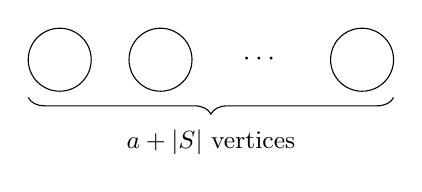
\begin{tikzpicture}[scale=0.8]
        % Isolated nodes
        \node[circle, draw, minimum size=0.8cm] (v1) at (0,0) {};
        \node[circle, draw, minimum size=0.8cm] (v2) at (1.6,0) {};
        \node at (3.2, 0) {$\cdots$};
        \node[circle, draw, minimum size=0.8cm] (v3) at (4.8,0) {};

        % Underbrace with label
        \draw [decorate, decoration={brace, amplitude=6pt, mirror}]
            (-0.5, -0.6) -- (5.3, -0.6)
            node[midway, below=8pt] {\small $a + |S|$ vertices};
    \end{tikzpicture}
    \caption{The decomposition graph $\graphform{\calA_{S}}$, which consists of $a + |S|$ isolated vertices.}
    \label{fig:decomp_graph_AS}
\end{figure}

\section{Proof of Proposition~\ref{pro:complexity_einsum}}
\label{app:complexity_einsum}

Our proposed algorithm for computing a tensor $\calT$ is based on iterating the \Einsum{} operation w.r.t. the corresponding \Einsum{} notation $\calA$, summing over one index at a time. We refer readers to Definition~\ref{def:tensor_expression} in the main text for the meaning of the index set of an \Einsum{} notation. 

On a high level, the proof proceeds by establishing a correspondence between the \Einsum{} notation and the associated decomposition graph (Definition~\ref{def:graph_decomp}). With the latter, we can leverage concepts from graph theory and combinatorics to obtain a time complexity upper bound of computing $\calT$. In particular, we will demonstrate that the summation over each index in the \Einsum{} notation corresponds to eliminating one vertex of the decomposition graph following Definition~\ref{def:vertex_elimination}. This characterization can help demonstrate that the treewidth of (Definition~\ref{def:treewidth_elimination}) the decomposition graph gives an optimistic estimate of the time complexity of the \Einsum{} operation.

To ease exposition, we decide to present the proof in a slow pace. The roadmap of the proof is as follows. We first construct a sequence of \Einsum{} notations, described in Definition~\ref{def:einsum_sequence} and Lemma~\ref{lem:einsum_graph_seq}, to mimic the computation procedure presented in Section~\ref{sec:alg_v}. Next, in Lemma~\ref{lem:complexity_one_index}, we obtain the computational complexity of summing over an index, which corresponds to the degree of the associated vertex in the decomposition graph. Finally, we complete the proof by showing that the optimal ordering of summation over indices is equivalent to identifying the best vertex elimination order of the decomposition graph. This is why the treewidth of the decomposition graph can be used to give an optimistic estimate of the time complexity.


\begin{definition}[\Einsum{} Notation Sequence]
\label{def:einsum_sequence}
Let $\calA = (A_1, \cdots, A_K)$ be an \Einsum{} notation (recall from Definition~\ref{def:tensor_expression}) with no output. Let $I = [m]$ be the index set of $\calA$ and $\sigma$ be a permutation over $I$. The \Einsum{} notation sequence of $\calA$ under $\sigma$ is the sequence $\calA^{\sigma}_0, \calA^{\sigma}_1, \ldots, \calA^{\sigma}_m$ defined recursively as follows:
\begin{itemize}
\item $\calA^{\sigma}_0 = \calA$.
\item For each $i \in I$, let $s_{\sigma[i]}$ be a permutation of the following set 
\begin{equation*}
    \bigcup_{\substack{ A \in \calA^{\sigma}_{i-1} \\ \sigma[i] \in A}} (\takesetp{A} \setminus \{\sigma[i]\}).
\end{equation*}. 
Then $\calA^{\sigma}_i$ is obtained from $\calA^{\sigma}_{i-1}$ by:
\begin{itemize}
\item Removing tuples in $\calA_{i - 1}^{\sigma}$ containing $\sigma[i]$.
\item Inserting $s_{\sigma[i]}$ as the last tuple into the tuple list if $s_j \ne \emptyset$.
\item Denoting the new tuple list as $\calA^{\sigma}_{i}$.
\end{itemize}
\end{itemize}
\end{definition}

We use the following concrete example to further illustrate the above definition. 

\begin{example}
Let $\calA = ((1,2), (1,3), (1,4), (2,3), (2,4), (3,4))$ and $\sigma = (1,2,3,4)$. Then the \Einsum{} notation sequence of $(\calA; \emptyset)$ under $\sigma$ is comprised of:
\begin{align*}
\calA^{\sigma}_{0} & = ((1,2), (1,3), (1,4), (2,3), (2,4), (3,4)), \\
\calA^{\sigma}_{1} & = ((2,3), (2,4), (3,4),(2,3,4)), \\
\calA^{\sigma}_{2} & = ((3,4), (3,4)), \\
\calA^{\sigma}_{3} & = ((4)), \\
\calA^{\sigma}_{4} & = (()).
\end{align*}
% Here in the first step, $j = \sigma[1] = 1$. So
% \begin{align*}
% \bigcup_{A \in \calA^{\sigma}_{0},\ 1 \in A} (\takesetp{A}  \setminus \{1\}) = \{2 , 4, 3\}
% \end{align*}
% and $\taketuplep{\{2 , 4, 3\}} = (2, 3, 4)$.
\end{example}

The following lemma establishes a one-to-one correspondence between the \Einsum{} notation sequence under a particular summation ordering $\sigma$ defined in Definition~\ref{def:einsum_sequence} and vertex elimination given in Definition~\ref{def:vertex_elimination}.

\begin{lemma}
\label{lem:einsum_graph_seq}
Let $\calA$ be an \Einsum{} notation with index set $I = [m]$ and $\sigma$ be a permutation of $I$. Let the sequence $\calA^{\sigma}_0, \calA^{\sigma}_1, \ldots, \calA^{\sigma}_m$ be the \Einsum{} notation sequence w.r.t. $\calA$ under permutation $\sigma$ (see Definition~\ref{def:einsum_sequence}) and $\graphform{\calA^{\sigma}_0}, \graphform{\calA^{\sigma}_1}, \ldots, \graphform{\calA^{\sigma}_m}$ be the corresponding decomposition graphs. Then for each $i \in [m]$, it holds that
\begin{align*}
   \graphform{\calA^{\sigma}_i} = \eliminatevg{\sigma[i]}{\graphform{\calA^{\sigma}_{i-1}}}.
\end{align*}
\end{lemma}

% \Zhang{should rewrite using induction}
\begin{proof}
Recalling from Definition~\ref{def:vertex_elimination} about the vertex elimination operation over a graph and Definition~\ref{def:graph_decomp} about the decomposition graph associated with a tuple list $\calA$ and tet $s_{\sigma[i]}$ be a permutation of the following set 
\begin{equation*}
    \bigcup_{\substack{ A \in \calA^{\sigma}_{i-1} \\ \sigma[i] \in A}} (\takesetp{A} \setminus \{\sigma[i]\}), 
\end{equation*}
we then recognize that removing all tuples containing $\sigma[i]$ from the tuple list $\calA^{\sigma}_{i - 1}$ corresponds to removing the vertex $\sigma[i]$ and all edges incident to $\sigma[i]$ in the decomposition graph $\graphform{\calA^{\sigma}_{i-1}}$ associated with $\calA^{\sigma}_{i-1}$ (some edges connected neighbors of $\sigma[i]$ may also be removed but will be re-added latter), while inserting the tuple $s_{\sigma[i]}$ into $\calA^{\sigma}_{i-1}$ corresponds connecting the neighbors of $\sigma[i]$ into a clique, which completes the proof. 
\end{proof}

\begin{lemma}
\label{lem:complexity_one_index}
Let $\calN = (\calA; B)$ be an \Einsum{} notation. Let $I = \indexset(\calN)$ and $m \coloneqq |I|$. Suppose that there is at least one common index $i$ in each $A_k$ and $B$ is a permutation of $I \backslash \{i\}$. Then for any tensors $\calT$ that can be represented by $\calN$ with each tensor of size $n$, the time complexity of computing $\tensorcontraction(\calT, \calN)$ is $\appequal(|\calA|n^{d})$.
\end{lemma}

\begin{proof}
We immediately have $|B| = d - 1$, which implies that the result of $\tensorcontraction(\calT, \calN)$ has $n^{d-1}$ entries. For each entry, as one index is summed over, it takes $n-1$ summation operations and $(|\calA|-1)n$ multiplication operations. Therefore, the total time complexity of computing $\tensorcontraction(\calT, \calN)$ is $\big((n-1)n^{d-1} + (|\calA|-1)n^d\big)$, which is $\appequal(|\calA|n^{d})$. 
\end{proof}

We need to introduce another notation before presenting the final proof: given two lists of tuples $\calA$ and $\calB$, we write $\calA \sqsubseteq \calB$ to mean that $\calA$ is a sublist of $\calB$.

\begin{proof}[Proof of Proposition~\ref{pro:complexity_einsum}]    
Let $m \coloneqq |\verticesp{G_\calA}|$. Let $\sigma$ be a permutation of $[m]$, and $\graphform{\calA^{\sigma}_0}, \graphform{\calA^{\sigma}_1}, \ldots, \graphform{\calA^{\sigma}_m}$ be the corresponding decomposition graphs. We define the $\calA^{\sigma}_0, \calA^{\sigma}_1, \ldots, \calA^{\sigma}_m$ be the \Einsum{} notation sequence under $\sigma$ as in Definition~\ref{def:einsum_sequence}.
    
We first show that there is an algorithm such that the time complexity of computing $\tensorcontraction(\calT, \calA)$ is $\less(n^{C_\sigma + 1}) $ where
\begin{equation*}
C_\sigma \coloneqq \max_{i \in [m]} \degp{\sigma[i]}{\graphform{\calA^{\sigma}_{i-1}}}.
\end{equation*}

To see this, we use \Einsum{} notation to characterize this procedure. First, for $i \in [m] \cup {0}$, we define the tensor tuple $\calT^\sigma_i$ corresponding to the \Einsum{} notation sequence $\calA^\sigma_i$ as follows: $\calT^{\sigma}_{0} \coloneqq \calT$ and for each $i \in [m]$:
\begin{itemize}
    \item $\sigma[i]$ is the index to be eliminated at the $i$-th step;
    \item Let $\calA^{\sigma, \mathrm{in}}_i \sqsubseteq \calA^{\sigma}_{i-1}$ be the sublist of $\calA^{\sigma}_{i-1}$ that contains $\sigma[i]$, i.e.
    \begin{align*}
    A \in \calA^{\sigma, \mathrm{in}}_i \iff \sigma[i] \in A,
    \end{align*}
    and similarly let $\calT^{\sigma, \mathrm{in}}_i \sqsubseteq \calT^{\sigma}_{i-1}$ be the tensor tuple corresponding to $\calA^{\sigma, \mathrm{in}}_i $;
    
    \item Let $B^{\sigma, \mathrm{out}}_i$ be a permutation of the set $\bigcup_{\substack{A \in \calA^{\sigma}_{i-1} \\ \sigma[i] \in A}} (\takesetp{A} \setminus \{\sigma[i]\})$ as the output tuple and $T^{\sigma, \mathrm{out}}_i \coloneqq \tensorcontraction(\calT^{\sigma, \mathrm{in}}_i, (\calA^{\sigma, \mathrm{in}}_i, B^{\sigma, \mathrm{out}}_i))$;
    
    \item Update the tensor tuple $\calT^{\sigma}_i$ from $\calT^{\sigma}_{i-1}$ by
    \begin{itemize}
        \item removing all tensors in $\calT^{\sigma, \mathrm{in}}_i$ from $\calT^{\sigma}_{i-1}$, and then
        \item inserting $T^{\sigma, \mathrm{out}}_i$ to the end of $\calT^{\sigma}_{i-1}$ to form $\calT^{\sigma}_{i}$.
    \end{itemize}
\end{itemize}

According to the distributive property of multiplication over summation, it holds that for any $i,j \in [m]$, 
\begin{align*}
\tensorcontraction(\calT^\sigma_i, \calA^\sigma_i) \equiv  \tensorcontraction(\calT^\sigma_j, \calA^\sigma_j) \equiv \tensorcontraction(\calT, \calA).
\end{align*}

Thus the time complexity of computing $\tensorcontraction(\calT, \calA)$ just comes from transferring from one step to the next step, which is $\tensorcontraction(\calT^{\sigma, \mathrm{in}}_i, (\calA^{\sigma, \mathrm{in}}_i, B^{\sigma, \mathrm{out}}_i))$. Following Lemma~\ref{lem:complexity_one_index}, we obtain that the time complexity of computing $\tensorcontraction(\calT^{\sigma, \mathrm{in}}_i, (\calA^{\sigma, \mathrm{in}}_i, B^{\sigma, \mathrm{out}}_i))$ is $\appequal(|\calA^{\sigma, \mathrm{in}}_i| n^{\degp{x}{\graphform{\calA^{\sigma}_{i-1}}}})$, which is also $\appequal(|\calA|n^{\degp{\sigma[i]}{\graphform{\calA^{\sigma}_{i-1}}}})$ as $|\calA^{\sigma, \mathrm{in}}_i| \leq |\calA|$. By taking maximum over $i$, the overall time complexity is thus $\less(|\calA|n^{C_\sigma + 1})$.

Finally, following Lemma~\ref{lem:einsum_graph_seq}, we have
\begin{align*}
\graphform{\calA^{\sigma}_i} = \eliminatevg{\sigma[i]}{\graphform{\calA^{\sigma}_{i-1}}},
\end{align*}
and by finding the permutation $\sigma^{\ast}$ minimizing $ C_{\sigma}$ and recalling Definition~\ref{def:treewidth_elimination}, we can conclude that there exists an algorithm such that the time complexity of $\tensorcontraction(\calT, \calA)$ is $\less(|\calA|n^{\treewidthp{G_\calA}+1})$, which completes the proof. 
\end{proof}

\iffalse
\begin{proof}[Proof of Proposition~\ref{pro:complexity_einsum}]
Let $m \coloneqq |\verticesp{G_\calA}|$. We recall that $G_{\calA}$ is the decomposition graph associated with the \Einsum{} notation $\calA$. Given a permutation $\sigma$ of the index set $I$, similar to Definition~\ref{def:treewidth_elimination}, we define graphs $G^\sigma_i, i \in [m] \cup \{0\}$ recursively as follows: 
\begin{itemize}
\item $G^\sigma_0 \coloneqq G_\calA$;
\item for $i \in [m]$, $G^\sigma_i \coloneqq \eliminatevg{\sigma[i]}{G^\sigma_{i-1}}$,  
where we again recall from Definition~\ref{def:vertex_elimination} about the definition of $\eliminatevg{j}{G}$, given a vertex index $j$ and a graph $G$.
\end{itemize}
And then define
\begin{align*}
C_\sigma \coloneqq \max_{i\in[m]}\degp{\sigma[i]}{G^\sigma_{i-1}},
\end{align*}
which is the maximum over the degrees of the vertices $\sigma[i]$ w.r.t. $G_{i - 1}^{\sigma}$ being eliminated during the above elimination process. Recalling Definition~\ref{def:treewidth_elimination}, 
\begin{align*}
    \max_{\sigma \in \perm{[m]}}C_\sigma = \treewidthp{G_\calA}. 
\end{align*}

We prove that there always exists an algorithm such that the time complexity of the contraction $\tensorcontraction(\calT, \calA)$ is $\less(n^{C_\sigma + 1})$. Our approach is as follows. First, we divide the computation of $\tensorcontraction(\calT,\calA)$ into $m$ steps by $\sigma$, where at each step one index in $\calA$ is summed over (and thus eliminated). Next, we show that moving from one step to the next corresponds to eliminating a vertex in the associated graph. Finally, by identifying the step with the largest computational cost, we complete the proof.

Each step of computation is characterized by a sequence of tensors $\calT^\sigma_i$ and a sequence of \Einsum{} notations $ \calA^\sigma_i$, for $i \in [m] \cup \{0\}$ recursively as follows:
\begin{itemize}
\item $\calT^\sigma_0 \coloneqq \calT$ and $\calN^\sigma_0 \coloneqq \calN$;

\item for $i \in [m]$:
\begin{itemize}
    \item First we construct a new tensor $T_{i}^{\sigma,\mathrm{out}} \coloneqq \tensorcontraction(\calT_i^{\sigma,\mathrm{in}}, (\calA_))$, where
    \begin{itemize}
        \item constructing $\calA^{\sigma, \mathrm{in}}_i$ 
    \end{itemize}
\end{itemize}
\end{itemize}


For $i \in \naturals: 0 \leq i \leq m-1$, at first we pick up inputs at $\calA^\sigma_i$ that has index $\sigma[i]$ in order. Then we construct \Einsum{} notation $\calN_{\sigma[i]}$, whose inputs are what we pick and output is a permutation of all indices in inputs except $\sigma[i]$. Let $\calT_i^{\mathrm{in}}$ be tensors corresponding to inputs of $\calN_{\sigma[i]}$ at $\calA^\sigma_i$ and $T_{\sigma[i]} \coloneqq \tensorcontraction(\calT_i^{\mathrm{in}}, \calN_{\sigma[i]})$. Then $\calT^\sigma_{i+1}$ and  $\calA^\sigma_{i+1}$ are constructed as follows:
\begin{itemize}
    \item Remove all tensors at $\calT_i^{\mathrm{in}}$ from $\calT^\sigma_i$ and add $T_{\sigma[i]}$ to the end of the latter. Then we get $\calT^\sigma_{i+1}$. 
    \item Remove all inputs appearing in inputs of $\calN_{\sigma[i]}$ from $\calA^\sigma_i$ and then add the output of $\calN_{\sigma[i]}$ to the end of the latter. Then we get $\calA^\sigma_{i+1}$
\end{itemize}

It holds that
\begin{align*}
    \tensorcontraction(\calT, \calA) & \equiv \tensorcontraction(\calT^\sigma_1, \calA^\sigma_1) \\
    & \equiv \cdots \\
    & \equiv \tensorcontraction(\calT^\sigma_m, \calA^\sigma_m),
\end{align*}
because of distributive property of multiplication over summation. 

Thus the whole procedure of computing $\tensorcontraction(\calT, \calA)$ is divided to a sequence of "smaller" \Einsum{} operation $\tensorcontraction(\calT_i^{\mathrm{in}}, \calN_{\sigma[i]}), 1 \leq i \leq m$. 

We prove that the time complexity of computing $\tensorcontraction(\calT_i^{\mathrm{in}},\calN_{\sigma[i]})$ is $\less(n^{\degp{\sigma[i]}{G^\sigma_{i-1}}+1})$. 
It is started with proving the decomposition graph of $\calA^\sigma_i$ is $G^\sigma_i$. Trivially it holds for $i=0$. Assume it holds for $i = j$. Then for $i=j+1$, recall procedure of constructing $\calA^\sigma_{j+1}$: when removing all inputs appearing in inputs of $\calN_{\sigma[j]}$ from $\calA^\sigma_j$, vertex $\sigma[j]$ is removed from $G^\sigma_j$ (some edges connected other vertices may also be removed but will be re-added latter); when adding the output of $\calN_{\sigma[j]}$ to the end of $\calA^\sigma_j$, the neighbors of vertex $\sigma[j]$ is connected to clique. This procedure corresponds to vertex elimination of a graph. Recalling the definition of $G^\sigma_j$, we complete the proof. 

Then we analyzing the complexity of computing $\tensorcontraction(\calT_i^{\mathrm{in}},\calN_{\sigma[i]})$. The result has $n^{N_i}$ entries, where $N_i$ is the length of the output of $\calN_{\sigma[i]}$, which is equal to the number of neighbors of $\sigma[i]$ at graph $G^\sigma_{i-1}$ and it needs $n-1$ summation operations and $\less(n)$ multiplication operations. Thus the complexity of computing $\tensorcontraction(\calT_i^{\mathrm{in}},\calN_{\sigma[i]})$ is $O(n^{N_i+1})$. As $N_i \equiv \degp{\sigma[i]}{G^\sigma_{i-1}}$, we complete the proof that the time complexity of computing $\tensorcontraction(\calT_i^{\mathrm{in}},\calN_{\sigma[i]})$ is $\less(n^{\degp{\sigma[i]}{G^\sigma_{i-1}}+1})$.

Taking the maximum complexity of the whole procedure, we obtain that there exists an algorithm, such that the time complexity of $\tensorcontraction(\calT, \calA)$ is $\less(n^{C_\sigma + 1})$.

Finally, there always exists an optimal permutation $\sigma_{\rm opt} \coloneqq \arg \min_{\sigma} C_{\sigma}$ that minimizes $C_\sigma$. Thus we can conclude that there exists an algorithm such that the time complexity of $\tensorcontraction(\calT, \calA)$ is $\less(n^{\treewidthp{G_\calA}+1})$ by recalling the definition of treewidth in Definition~\ref{def:treewidth_elimination}. Hence we conclude that an optimistic estimate of the time complexity of $\tensorcontraction(\calT, \calA)$ is $\less(n^{\treewidthp{G_\calA}+1})$.
\end{proof}
\fi
\iffalse
Consider the first step where we sum over index $j \coloneqq \sigma[1]$. Let $\calA^{\sigma, \mathrm{in}}_{1}$ be the list of tuples containing $j$ and $\calT^{\sigma, \mathrm{in}}_{1}$ be the corresponding tuple of tensors, i.e.:
    \begin{equation*}
    A \in \calA^{\sigma, \mathrm{in}}_{1} \sqsubseteq \calA^{\sigma}_0 \iff j \in A,
    \end{equation*}
    and let $B^{\sigma, \mathrm{out}}_{1}$ be the output tuple: 
    \begin{equation*}
    B^{\sigma, \mathrm{out}}_{1} = \taketuplep{\bigcup_{A \in \calA^{\sigma}_{0},\ j \in A} (\takesetp{A} \setminus \{j\}) }. 
    \end{equation*}
    Summing over the index $j = \sigma[1]$ can then be expressed as $T^{\sigma,\mathrm{out}}_{1} = \tensorcontraction(\calT^{\sigma, \mathrm{in}}_{1}, (\calA^{\sigma, \mathrm{in}}_{1}, B^{\sigma, \mathrm{out}}_{1}))$, where by the definition of decomposition graph (Definition~\ref{def:graph_decomp}), $|\indexset(\calA^{\sigma, \mathrm{in}}_{1})| = \degp{j}{\graphform{\calA^{\sigma}_0}} + 1$ and $|\takesetp{B^{\sigma, \mathrm{out}}_{1})}| = \degp{j}{\graphform{\calA^{\sigma}_0}}$. By Lemma~\ref{lem:complexity_one_index}, the time complexity of this summation is $\less(n^{\degp{j}{\graphform{\calA^{\sigma}_0}}} )$. 
    
    In the second step, we have a new tensor $T^{\sigma,\mathrm{out}}_{1}$, which is the output from the first step and we need to remove the used subtuple of tensors $\calT^{\sigma, \mathrm{in}}_{1}$. The new tensor tuple denoted as $\calT^{\sigma}_{1}$ can then be constructed by:
    \begin{itemize}
    \item first removing all tensors in $\calT^{\sigma, \mathrm{in}}_1$ from $\calT_{0}^{\sigma}$; and
    \item inserting $T^{\sigma,\mathrm{out}}_1$ as the first tensor into $\calT_{0}^{\sigma}$ to finally form $\calT^{\sigma}_{1}$.
    \end{itemize}
    \Zhang{the above procedure should have been completed in the first step.}
    The following identity holds:
    \begin{align*}
    \tensorcontraction(\calT, \calA) \equiv \tensorcontraction(\calT^\sigma_1, \calA^\sigma_1) 
    \end{align*}
    due to the distributive property of multiplication over summation. But by construction, $\tensorcontraction(\calT^\sigma_1, \calA^\sigma_1)$ has one fewer index than $\tensorcontraction(\calT, \calA)$. 
    Now we can describe the $i$-th step of the whole procedure under the summation ordering $\sigma$ as below.
\fi


\section{Proof of Lemma~\ref{lem:decomp_u_to_v}}
\label{app:decomp_u_stats}

Here we prove an extended version of Lemma~\ref{lem:decomp_u_to_v}, as shown in Lemma~\ref{lem:ext_decomp_u_to_v} below. Lemma~\ref{lem:decomp_u_to_v} then becomes a simple corollary of Lemma~\ref{lem:ext_decomp_u_to_v}. We begin by introducing the following definitions.

\begin{definition}[Refinement of Partitions]\label{def:refinement_of_partition}
Let $\sPi$ and $\rho$ be two partitions of a non-empty set $S$. $\sPi$ is said to be finer than $\rho$, if for any $A \in \sPi$, there exists $B \in \rho$ such that $A \subseteq B$, denoted by $\sPi \pleq \rho$. Additionally, $\sPi$ is strictly finer than $\rho$ if $\sPi \neq \sPi$, denoted by $\rho \pless \sPi$. 
\end{definition}

\begin{remark}
Refinement defines a partial order on partitions of a set and in fact forms a \emph{partition lattice}, a classical result in lattice theory \citep{birkhoff1940lattice}. 
\end{remark}

Similar to restricted $V$-statistics defined in Definition~\ref{def:res_v_stat}, we define U-set and restricted $U$-statistics as follows. 

\begin{definition}[U-Set]\label{def:u_set}
Let $m,n$ be positive integers satisfying $m \leq n$ and $\sPi$ be a partition of the set $[m]$. A U-set of size $n$ w.r.t. the partition $\sPi$ is defined as
    \begin{align*}
        \usetnm{n}{\sPi} \coloneqq \left\{ \overline{s}_m \in [n]^m \mid \text{where for any $i, j \in [m]$}, i, j \in Q \text{ for some $Q \in \sPi$} \iff   s_i = s_j \right\}.
    \end{align*}
    If $\sPi$ happens to be the finest partition of $[m]$, i.e. $\sPi = \{\{1\}, \{2\}, \cdots, \{m\}\}$, the corresponding U-set is denoted by $\uset(n,m)$ and in fact, $\uset(n,m) \equiv \perm{n,m}$. The cardinality of the given partition $\sPi$ is referred to as the order of $\usetnm{n}{\sPi}$.
\end{definition}

\begin{definition}[Restricted $U$-Statistic]\label{def:res_u_stats}
    Let $\bbX$ be a non-empty set, $m, n$ be positive integers satisfying $m \leq n$, $\sPi$ be a partition of set $[m]$ and $h: \bbX^{m} \rightarrow \bbR$ be a function defined on $\bbX^m$. For any tuple $\bm{X} \in \bbX^n: n \geq m$, the $U$-statistic with kernel $h$ restricted by partition $\sPi$ takes the following form 
    \begin{align*}
        \ustat[\pi](h, \bm{X}) \coloneqq \sum_{\alpha \in \uset(n,\pi)} h(\bm{X}[\alpha]). 
    \end{align*}
\end{definition}

Armed with Definitions~\ref{def:refinement_of_partition} -- \ref{def:res_u_stats}, we are ready to present the following extended form of Lemma~\ref{lem:decomp_u_to_v}. 

\begin{lemma}[Extended Form of Lemma~\ref{lem:decomp_u_to_v}]
\label{lem:ext_decomp_u_to_v}
    Let
    \begin{itemize}
        \item $\samplespace$ be a non-empty set,
        \item $m,n$ be integers satisfying $m \leq n$,
        \item $h$ be a function defined on $\samplespace^m$,
        \item $\bm{X} \in \samplespace^n$. 
    \end{itemize}
    Then for any $\sPi \in \partitionp{m}$, it holds that
    \begin{align*}
        \ustat[\sPi](h,\bm{X}) 
        = \sum_{\substack{ \rho \in \partitionp{m} \\ \sPi \pleq \rho }}  
        \mu(\sPi, \rho)  \vstat[\rho](h, \bm{X}),
    \end{align*}
    where the coefficients $\mu(\sPi, \rho)$ are given by
    \begin{align*}
        \mu(\sPi, \rho) 
        = (-1)^{|\sPi|-|\rho|} 
        \prod_{C \in \rho} (\kappa_{\sPi, C} - 1)!, \text{ and } \kappa_{\sPi, C} \coloneqq |\{ Q \in \sPi \mid Q \subseteq C \}|.
    \end{align*}
    In particular, if $\sPi$ happens to be $\{\{k\} \mid k \in [m]\}$, the above result reduces to Lemma~\ref{lem:decomp_u_to_v}. 
\end{lemma}

The proof of Lemma~\ref{lem:ext_decomp_u_to_v} can be found in Appendix~\ref{app:proof_ext_decomp_u_to_v}.

\subsection{Preparatory Materials}\label{app:preparatory_materials}

Before presenting the proof in the next section, we introduce some useful preparatory materials, including: (1) the decomposition of a $V$-statistic into $U$-statistics and (2) a dual form of \mobius{} inversion formula \citep{stanley2011enumerative}. We first state the following technical result of decomposing a $V$-statistic into a linear combination of $U$-statistics. 
\begin{lemma}[Decomposition of $V$-Statistic into $U$-Statistics]
\label{lem:decomp_v_to_u}
    Let
    \begin{itemize}
        \item $\samplespace$ be a non-empty set, 
        \item $m,n$ be positive integers satisfying $m \leq n$, 
        \item $h$ be a function defined on $\bbX^m$, 
        \item $\bm{X} \in \samplespace^n$. 
    \end{itemize}
    Then for any $\sPi \in \partitionp{m}$, it holds that
    \begin{align*}
        \vstat[\sPi](h, \bm{X}) = \sum_{\substack{
            \rho \in \partitionp{m} \\ \sPi \pleq \rho
        }} \ustat[\rho](h,\bm{X}),
    \end{align*}
    where
     \begin{align*}
       \ustat[\rho](h,\bm{X}) = \sum_{\alpha \in \usetnm{n}{\rho}} h(\bm{X}[\alpha]). 
    \end{align*}
\end{lemma}

\begin{proof}
It is equivalent to prove that $\{\usetnm{n}{\rho} \mid \rho \in \partitionp{m}: \sPi \pleq \rho\}$ forms a partition (i.e. disjoint union) of $\vsetp{n}{\sPi}$, i.e.
\begin{align*}
\vsetp{n}{\sPi} = \bigsqcup_{\substack{\rho \in \partitionp{m} \\ \sPi \pleq \rho} }\usetnm{n}{\rho}.
\end{align*}

    {\bf Part 1: Disjointness}
    
    We first prove that for any $\pi_1, \pi_2 \in \{\rho \in \partitionp{m} \mid \sPi \pleq \rho \}: \pi_1 \neq \pi_2$, it holds that
    \begin{align*}
        \usetnm{n}{\pi_1} \cap \usetnm{n}{\pi_2} = \emptyset. 
    \end{align*}

    Since $\pi_1 \neq \pi_2$, there must exist $i_1, i_2 \in [m]$ such that either
    \begin{itemize}
        \item $\exists \, Q_1 \in \pi_1$, such that $i_1, i_2 \in Q_1$, and
        \item $\forall \, Q_2 \in \pi_2$, $i_1, i_2 \notin Q_2$, 
    \end{itemize}
    or 
    \begin{itemize}
        \item $\forall \, Q_1 \in \pi_1$, $i_1, i_2 \notin Q_1$, 
        \item $\exists \, Q_2 \in \pi_2$, such that $i_1, i_2 \in Q_2$.  
    \end{itemize}
    Without loss of generality, we assume that the former holds. Following Definition~\ref{def:u_set}, we have for any $\alpha_1 \in \usetnm{n}{\pi_1}$, $\alpha_1[i_1] = \alpha_1[i_2]$, but for any $\alpha_2 \in \usetnm{n}{\pi_2}$, $\alpha_1[i_1] \neq \alpha_1[i_2]$, which implies that $\usetnm{n}{\pi_1} \cap \usetnm{n}{\pi_2} = \emptyset$. 

    {\bf Part 2: Coverage}

    We are left to prove that for any $\alpha \in \vsetp{n}{\sPi}$, there exists $\rho \in \partitionp{m}: \sPi \pleq \rho$, such that $\alpha \in \usetnm{n}{\rho}$. We first construct a candidate $\rho$ as follows. For each $j \in \takesetp{\alpha}$, let
    \begin{align*}
    Q_j \coloneqq \{i \in [m] \mid \alpha[i] = j\},
    \end{align*}
    and then let $\rho \coloneqq \{Q_j \mid j \in \takesetp{\alpha}\}$. It is straightforward to verify that $\rho$ is a partition of $[m]$. 
    
    Then we prove that $\rho$ is the partition satisfying the desiderata. Following Definition~\ref{def:u_set}, we have $\alpha \in \usetnm{n}{\rho}$. Following Definition~\ref{def:v_set}, we have for any $Q \in \sPi$ and any $i_1, i_2 \in Q$, $\alpha[i_1] = \alpha[i_2]$, which implies that for any $Q \in \pi$, $Q \subseteq B_{j_Q} \in \rho$, for some $j_Q$ such that
    \begin{align*}
        \alpha[j_Q] = \alpha[i], \quad \forall \, i \in Q, 
    \end{align*}
    We then obtain that $\sPi \pleq \rho$ following Definition~\ref{def:refinement_of_partition}, which complete the proof of coverage. 

    Combining Part 1 and Part 2, we complete the proof of this lemma. 
\end{proof}

Next, we introduce the notion of \mobius{} inversion formula, which is used to reverse the decomposition from a $V$-statistic into $U$-statistics in Lemma~\ref{lem:decomp_v_to_u} to obtain the decomposition from a $U$-statistic into $V$-statistics.

\begin{definition}[\mobius{} Function, \cite{stanley2011enumerative}]\label{def:mobius_func}
    Let $(P, \preceq)$ be a finite poset and, a function $\mu: P^2 \to \reals$ is said to be a \mobius{} function on $(P, \preceq)$, if
    \begin{align*}
        \mu(s,s) = & \ 1, \quad \forall \ s \in P, \text{ and} \\
        \mu(s,u) = & - \sum_{\substack{t \in P \\ s \preceq t \prec u}} \mu(s,t), \quad \forall \ s, u \in P: s \prec u.
    \end{align*}
\end{definition}

\begin{lemma}[\mobius{} Function on Partition Lattices, \cite{stanley2011enumerative}]\label{lem:mobius_func_partition}
Let $S$ be a non-empty set. Then the \mobius{} function on $(\partitionp{S}, \pleq)$ takes the following form
\begin{align*}
    \mu(\sPi, \rho) = (-1)^{|\sPi|-|\rho|} \prod_{C \in \rho} (\kappa_{\sPi, C} - 1)!, \quad \forall \, \sPi,\rho \in \partitionp{S}: \sPi \pleq \rho \text{ and } \kappa_{\sPi, C} = |\{ A \in \sPi \mid A \subseteq C \}|.
\end{align*}
\end{lemma}

\begin{lemma}[\mobius{} Inversion Formula, Dual Form,  \cite{stanley2011enumerative}]\label{lem:mobius_formula_dual}
    Let $(P, \preceq)$ be a finite poset and $f, g$ be functions defined on $P$. Then
    \begin{align*}
        g(s) = \sum_{\substack{t \in P \\ s \preceq t}}f(t), \quad \forall \, s \in P,
    \end{align*}
    if and only if
    \begin{align*}
        f(s) = \sum_{\substack{t \in P \\ s \preceq t}} \mu(s,t)g(t), \quad \forall \, s \in P, 
    \end{align*}
    where $\mu$ is the \mobius{} function on $(P, \preceq)$. 
\end{lemma}

\subsection{Proof of Lemma~\ref{lem:ext_decomp_u_to_v}}
\label{app:proof_ext_decomp_u_to_v}

In this section, we prove Lemma~\ref{lem:ext_decomp_u_to_v}. The argument is straightforward given the preparations in the previous section.

\begin{proof}[Proof of Lemma~\ref{lem:ext_decomp_u_to_v}]
If we fix $h$ and $\bm{X}$, $f(\sPi) \coloneqq \ustat[\sPi](h,\bm{X})$ and $g(\rho) \coloneqq \vstat[\rho](h,\bm{X})$ are functions defined on $\partitionp{m}$. 

Since $\partitionp{m}$ is finite and the refinement defined in Definition~\ref{def:refinement_of_partition} defines a partial order on $\partitionp{m}$, we can apply Lemma~\ref{lem:mobius_formula_dual} to functions $f$ and $g$. 

Combining the \mobius{} function on $\partitionp{m}$ as stated in Lemma~\ref{lem:mobius_func_partition}, the dual form of \mobius{} inversion formula given in Lemma~\ref{lem:mobius_formula_dual} and the relationship between $f$ and $g$ as stated in Lemma~\ref{lem:decomp_v_to_u}, we immediately complete the proof. 
\end{proof}


\section{An Open Problem}
\label{app:open}

In this section, we present an open problem that we ourselves find intriguing. As we indicated in Remark~\ref{rem:tw} at the end of Section~\ref{sec:alg_u_v}, the treewidth of the decomposition graph associated with the \Einsum{} notation of the underlying $V$-statistic relates to its time complexity. But the treewidth of a graph is not easy to compute either analytically \citep{harvey2018treewidth} or numerically \citep{arnborg1987complexity}. It will be interesting to get a sharp bound on treewidth using the number of vertices or edges of the graph. As mentioned in Remark~\ref{rem:tw}, \citet{kneis2009bound} has shown that the treewidth is bounded at most linearly by the edge size, or more precisely bounded by $e / 5.769 + O (\log n)$ where $n \coloneqq |V|$ denotes the number of vertices in $G$. However, we do not know whether this bound can be further improved. Below we provide the maximum tree-width that is possible for a graph with edge size no greater than $15$, to hopefully serve as a starting point of fully addressing this problem.
\begin{observation}[Treewidth and Edge Count]
\label{pro:treewidth_table}
Let
\begin{equation*}
\mathrm{t}(e) \coloneqq \max \left\{ \treewidthp{G} \;\middle|\; G \text{ is a graph where } |E(G)| = e \right\}.
\end{equation*}
We have computed the exact values of $\mathrm{t} (e)$ for all $1 \le e \le 15$ as follows:
\begin{equation*}
\begin{split}
\mathrm{t} (e) = \left\{ \begin{array}{ll}
1, & e \in \{1, 2\}, \\
2, & e \in \{3, 4, 5\}, \\
3, & e \in \{6, 7, 8, 9\}, \\
4, & e \in \{10, 11, 12, 13, 14\}, \\
5, & e = 15.
\end{array} \right.
\end{split}
\end{equation*}
\end{observation}
The proof can be found in Appendix~\ref{app:treewidtg_table}. However, extending the above result to $e > 15$ is currently beyond our reach.

\section{Proof of Observation~\ref{pro:treewidth_table}}
\label{app:treewidtg_table}


We begin by recalling some well-known bounds on treewidth. We then restrict our attention to simple graphs without isolated vertices and derive recurrence relations in several basic cases. The final proof proceeds by carefully verifying the conditions of Lemma~\ref{lem:property_of_tt} to be stated below.

\begin{definition}[Degeneracy]
\label{def:degeracy}
The \emph{degeneracy} of a graph $G$, denoted by $\degeneracyg{G}$, is defined as the maximum value of the minimum degree $\delta(H)$ over all subgraphs $H$ of $G$.
\end{definition}

We first present some results on inequalities involving treewidth. The first two inequalities are from \citet{bodlaender2011treewidth}, while the last one follows directly from Definition~\ref{def:treewidth_elimination}.

\begin{lemma}
\label{lem:simple_bounds_on_treewidth}
Let $G = (V, E)$ be a graph. Then
\begin{enumerate}
    \item $ \degeneracyg{G} \leq \treewidthp{G},$
    
    \item if $H$ is a subgraph of $G$, then $\treewidthp{H} \leq \treewidthp{G}$, 
    
    \item for any vertex $v \in V$, it holds that $\treewidthp{G} \leq \max \{\degp{v}{G}, \treewidthp{\eliminatevg{v}{G}} \}$.
\end{enumerate}
\end{lemma}

We then present results concerning the treewidth of graphs subject to constraints on the number of edges or vertices.

\begin{lemma}
\label{lem:property_of_tt}
Let $\graphsetne{n}{e}$ be the set of all simple graphs with $n$ vertices, $e$ edges, and no isolated vertices, and let $\graphsetne{n}{e} = \emptyset$ if no such graphs exist. Let $\mathrm{tt}(n, e)$ denote the maximum treewidth of the graphs in $\graphsetne{n}{e}$:
\begin{equation*}
\mathrm{tt}(n, e) \coloneqq \max\left\{ \treewidthp{G}\;\middle|\; G \in \graphsetne{n}{e} \right\}.
\end{equation*}
The following properties hold:
\begin{enumerate}
    \item \textbf{Support set:} For any fixed $e \in \positivenaturals $, $\graphsetne{n}{e}$ is nonempty if and only if 
    \begin{equation*}
        n \in \mathrm{n}(e) \coloneqq \left\{ n \in \positivenaturals \, \middle \vert\,  \binom{n}{2} \geq e,  n \leq 2e \right\}.
    \end{equation*}
    \item \textbf{Representation of $\mathrm{t}(e): $} $ \mathrm{t}(e) = \max_{n \in \mathrm{n}(e)} \mathrm{tt} (n, e).$
    \item \textbf{Monotonicity in edge counts:} For any fixed $n: n \in \mathrm{n}(e+1) $, the function $\mathrm{tt}(n, e)$ is non-decreasing w.r.t. $e$.
    \item \textbf{Treewidth of complete graph:} $\mathrm{tt}(n, \binom{n}{2}) =  n - 1$, $\mathrm{tt}(n, \binom{n}{2} - 1) = n - 2$.
    \item \textbf{Recurrence relations in simple cases:}  recall that $\frac{2e}{n}$ is in fact the average degree of the graph and when $e > 2$ and $n \in \mathrm{n} (e)$:
    \begin{itemize}
        \item[(1)] If $1 \leq \frac{2e}{n} < 2$, then $ \mathrm{tt}(n,e) \leq \max\{ 1, \mathrm{t}(e-1) \}$.
        \item[(2)] If $1 \leq \frac{2e}{n} < 3$, then $ \mathrm{tt}(n,e)  \leq \max\{ 2, \mathrm{t}(e-1) \} $.
        \item[(3)] If $1 \leq \frac{2e}{n} < 4$, then $ \mathrm{tt}(n,e)  \leq \max\{ 3, \mathrm{tt}(n - 1 ,e), \mathrm{t}(e-1) \}$.
        \item[(4)] $ \mathrm{tt}(7,14) \leq  \max\{ 4,  \mathrm{t}(13) \}$.
    \end{itemize}
\end{enumerate}
\end{lemma}

\begin{proof}
We prove the lemma in the following steps.
    \begin{enumerate}
    \item Since a simple graph with $n$ vertices and no isolated vertices can have at most $\binom{n}{2}$ edges, we must have $e \leq \binom{n}{2}$. Moreover, as isolated vertices are not allowed, every vertex must have degree at least one. In particular, the average degree satisfies $\frac{2e}{n} \geq 1$, which implies $n \leq 2e$.

    \item The definition of $\mathrm{t}(e)$ does not exclude graphs with isolated vertices. However, for any graph $G$ with $e$ edges and isolated vertices, eliminating those vertices (with degree 0) does not affect the number of edges or the treewidth. Therefore, it suffices to take the maximum over all graphs in $\graphsetne{n}{e}$ for $n \in \mathrm{n}(e)$, i.e. taking the maximum over $\mathrm{tt}(n,e)$ for $n \in \mathrm{n}(e)$.

    \item We observe that any graph $G \in \graphsetne{n}{e}$ can be extended to a graph $G^\prime \in \graphsetne{n}{e+1}$ by adding an edge, since $n \in \mathrm{n}(e+1)$. By the subgraph monotonicity of treewidth stated in Lemma~\ref{lem:simple_bounds_on_treewidth}, it follows that $\treewidthp{G} \leq \treewidthp{G^\prime}$. Therefore, we have $\mathrm{t}(e) \leq \mathrm{t}(e+1)$.
    
    \item First, consider the case where $e = \binom{n}{2}$. The only graph (up to isomorphism) with $n$ vertices and $\binom{n}{2}$ edges is the complete graph $K_n$. Since the degeneracy of $K_n$ is $n - 1$, we have $\treewidth(K_n) \geq n - 1$. To show the upper bound, note that eliminating any vertex in $K_n$ removes a vertex of degree $n - 1$ and yields $K_{n-1}$. By the third bound in Lemma~\ref{lem:simple_bounds_on_treewidth}, we get $\treewidth(K_n) \leq \max\{n - 1, \treewidth(K_{n-1})\}$. Repeating this process down to $K_2$, we have $\treewidth(K_n) \leq \max\{n - 1, \dots, \treewidth(K_2)\} = n - 1$, since $\treewidth(K_2) = 1$ is easy to verify. Therefore, $\mathrm{tt}(n, \binom{n}{2}) = n - 1$. 

    Next, consider $e = \binom{n}{2} - 1$. There is still only one graph in this case (up to isomorphism), obtained by deleting one edge from $K_n$. In this graph, two vertices have degree $n - 2$ and the rest have degree $n - 1$. Since it contains $K_{n-1}$ as a subgraph, we have a lower bound $\treewidth \geq n - 2$ by the degeneracy. For the upper bound, eliminating one of the vertices with degree $n - 2$ yields $K_{n-2}$. Thus, $\treewidth \leq \max\{n - 2, \treewidth(K_{n-2})\} = n - 2$. Therefore, $\mathrm{tt}(n, \binom{n}{2} - 1) = n - 2$.

    \item Let us introduce another notation: let $\graphset_e \coloneqq \bigcup_{n \in \mathrm{n}(e)} \graphsetne{n}{e}$.

    \textbf{Case (1): $1 \leq \frac{2e}{n} < 2$}, the minimum degree in any graph in $\graphsetne{n}{e}$ must be exactly $1$. Eliminating such a vertex removes exactly one edge and yields a graph in $\graphset_{e - 1}$. Therefore, by the third bound in Lemma~\ref{lem:simple_bounds_on_treewidth}, we have $\mathrm{tt}(n,e) \leq \max\{1, \mathrm{t}(e - 1)\}$.

    \textbf{Case (2): $1 \leq \frac{2e}{n} < 3$}, the minimum degree in any graph from $\graphsetne{n}{e}$ must be either $1$ or $2$. If the minimum degree is $2$, eliminating such a vertex removes two edges (if its neighbors are adjacent) or one edge (if they are not, in which case we need to add one edge to connect them), and in both cases, one vertex is removed. The resulting graph lies in either $\graphsetne{n-1}{e-1}$ or $\graphsetne{n-1}{e-2}$. On the other hand, if the minimum degree is $1$, then as in the previous case, eliminating that vertex removes one edge and results in a graph in $\graphset_{e-1}$.     Therefore, by the vertex elimination bound (Lemma~\ref{lem:simple_bounds_on_treewidth}), we have $\mathrm{tt}(n,e) \leq \max\{2, \mathrm{t}(e - 1), \mathrm{tt}(n-1, e - 1), \mathrm{tt}(n-1, e - 2)\}$. Since $\mathrm{tt}(n-1, e - 2) \leq \mathrm{tt}(n-1, e - 1) \leq \mathrm{t}(e - 1)$, we conclude $\mathrm{tt}(n,e) \leq \max\{2, \mathrm{t}(e - 1)\}$.

    \textbf{Case (3): $1 \leq \frac{2e}{n} < 4$}. The minimum degree in any graph from $\graphsetne{n}{e}$ must be either $1$, $2$, or $3$. If the minimum degree is $3$, then eliminating such a vertex removes between $0$ and $3$ edges, depending on the connectivity of its neighbors, but in all cases it only removes exactly one vertex. Therefore, the resulting graph lies in $\graphsetne{n-1}{e}$, $\graphsetne{n-1}{e-1}$, $\graphsetne{n-1}{e-2}$, or $\graphsetne{n-1}{e-3}$. Combining this with the previous cases for minimum degree $1$ and $2$, we obtain the recurrence relation: $\mathrm{tt}(n,e) \leq \max\{3, \mathrm{tt}(n-1,e), \mathrm{tt}(n-1,e-1), \mathrm{tt}(n-1,e-2), \mathrm{tt}(n-1,e-3), \mathrm{t}(e-1)\} \leq \max\{3, \mathrm{tt}(n-1,e), \mathrm{t}(e-1)\}$.

    \textbf{Case (4): $n = 7$, $e = 14$}. First we observe that $\frac{2e}{n} = 4$, so the minimum degree in any graph $G = (V, E)$ from $\graphsetne{n}{e}$ must be $1$, $2$, $3$, or $4$.
    
    We focus on the case where the minimum degree is $4$, and argue that in this case, there must exist a vertex $v_1$ of degree exactly $4$ such that eliminating $v_1$ does not increase the number of edges.
    
    In general, eliminating a vertex of degree $4$ may remove 4 edges and add up to $\binom{4}{2} = 6$ fill-in edges among its neighbors, so the net change in edge counts, denoted by $\Delta_e$, ranges from $-4$ to $+2$. We now show that in our setting, increasing the number of edges (i.e., $\Delta_e > 0$) is impossible.
    
    Let $v_1$ be a vertex of degree $4$, and denote its neighborhood as $\{v_2, v_3, v_4, v_5\} = \neighborvg{v_1}{G}$. Partition the vertex set as $V = \{v_1\} \cup \{v_2, v_3, v_4, v_5\} \cup \{v_6, v_7\}$.
    
    Suppose that eliminating $v_1$ leads to $\Delta_e = 2$. This implies that $\neighborvg{v_1}{G}$ contains no edges, so 6 fill-in edges are added, making the neighborhood a clique. Now we count the maximum possible number of edges under this configuration:
    the 4 edges incident to $v_1$,
    no edges inside $\{v_2, v_3, v_4, v_5\}$,
    up to 1 edge inside $\{v_6, v_7\}$, and
    at most $2 \cdot 4 = 8$ edges between $\{v_6, v_7\}$ and $\{v_2, v_3, v_4, v_5\}$. Hence, the total number of edges is at most $4 + 0 + 8 + 1 = 13 < 14 = e$, contradicting the assumption. Therefore, $\Delta_e = 2$ is impossible.
    
    Now consider the case where eliminating $v_1$ leads to $\Delta_e = 1$. Then $\neighborvg{v_1}{G}$ must contain exactly one edge, say connecting $v_2$ and $v_3$, and the edges between $\{v_6, v_7\}$ and $\{v_2, v_3, v_4, v_5\}$ and inside $\{v_6, v_7\}$ all appear. This allows a maximum of $4 + 1 + 8 + 1 = 14$ edges. However, in this setting, $v_4$ and $v_5$ are not adjacent to each other or to $v_2$ or $v_3$, and their neighbors are only in $\{v_1, v_6, v_7\}$. Thus, each of them has degree at most $3$, contradicting the assumption that the minimum degree is $4$.
    
    Combining the above arguments, we conclude that eliminating $v_1$ does not increase the number of edges. Hence, if the minimum degree is $4$, then there exists a vertex of degree $4$ such that eliminating this vertex yields a graph in $\graphsetne{n-1}{e'}$ with $e' \leq e$.
    
    Now combining this with previous arguments for when the minimum degree is $1$, $2$, or $3$, we obtain the recurrence relation: $ \mathrm{tt}(n, e) \leq \max\{4, \mathrm{tt}(n - 1, e), \mathrm{tt}(n - 1, e - 1), \mathrm{tt}(n - 1, e - 2), \mathrm{tt}(n - 1, e - 3), \mathrm{tt}(n - 1, e - 4), \mathrm{t}(e - 1)\} \leq \max \{ 4, \mathrm{tt}(n - 1, e),\mathrm{t}(e - 1) \}$.

    Since $\mathrm{tt}(n - 1, e) = \mathrm{tt}(6, 14) = 4$ by Property~4 shown earlier, we conclude: $\mathrm{tt}(7, 14) \leq \max\{4, \mathrm{t}(13)\}$.


    \end{enumerate} 
\end{proof}

Armed with the above results on treewidth, we prove Observation~\ref{pro:treewidth_table}.
\begin{proof}[Proof of Observation~\ref{pro:treewidth_table}]

We verify the values of $\mathrm{t}(e)$ for each $1 \le e \le 15$ by analyzing the sets $\graphsetne{n}{e}$ and showing that the lower and upper bounds coincide. Let $\mathrm{u}(e)$ (resp. $\mathrm{l}(e)$) denote the target upper (resp. lower) bound of $\mathrm{t}(e)$ for each $e$. Our goal is to prove that $\mathrm{t}(e) = \mathrm{l}(e) = \mathrm{u} (e)$ for all $e \in \{1, 2, \dots, 15\}$.

    \textbf{Lower bound.} For each $e$, a specific graph $G_e$ is provided in Figure~\ref{fig:treewidth_table}. Each $G_e$ is a simple graph with $e$ edges and contains a clique $\completegraphp{\mathrm{l}(e)+1}$ as a subgraph. By the definition of degeneracy and Lemma~\ref{lem:simple_bounds_on_treewidth}, we have:
    \begin{equation*}
        \mathrm{l}(e) \leq \degeneracyg{G_e} \leq \treewidthp{G_e} \leq \mathrm{t}(e).
    \end{equation*}

   \textbf{Upper bound.} We now show that $\mathrm{t}(e) \leq \mathrm{u}(e)$ by bounding $\mathrm{tt}(n,e)$ for all $n \in \mathrm{n}(e)$, using the properties in Lemma~\ref{lem:property_of_tt}.

From Property~4, we obtain:
\begin{align*}
    \mathrm{tt}(2,1) & = 1, \mathrm{tt}(3,3) = 2, \mathrm{tt}(4,6) = 3, \\ \mathrm{tt}(5,10) & = 4, \mathrm{tt}(6,15) = 5, \mathrm{tt}(5,9) = 3, \mathrm{tt}(6,14) = 4.
\end{align*}

\textbf{Case $e = 1, 2$:}

We have $\mathrm{n}(1) = \{2\}$ and $\mathrm{n}(2) = \{3, 4\}$, so:
\begin{equation*}
    \mathrm{t}(1) = \mathrm{tt}(2,1) = 1.
\end{equation*}

For $e = 2$, both $n = 3$ and $n = 4$ satisfy $1 \leq \frac{2e}{n} < 2$. By Property~5:
\begin{align*}
    \mathrm{tt}(3,2) &\leq \max\{1, \mathrm{t}(1)\} = 1, \\
    \mathrm{tt}(4,2) &\leq \max\{1, \mathrm{t}(1)\} = 1,
\end{align*}
and hence,
\begin{equation*}
    \mathrm{t}(2) = 1.
\end{equation*}

\textbf{Case $e = 3, 4, 5$:}

The support sets are:
\begin{align*}
    \mathrm{n}(3) &= \{3, 4, 5, 6\}, \\
    \mathrm{n}(4) &= \{4, 5, 6, 7, 8\}, \\
    \mathrm{n}(5) &= \{4, 5, \dots, 10\}.
\end{align*}
Observe that
\begin{equation*}
    \mathrm{n}(3) \setminus \{3\} \subseteq \mathrm{n}(4) \subseteq \mathrm{n}(5).
\end{equation*}

By monotonicity (Part 3 in Lemma~\ref{lem:property_of_tt}), we have:
\begin{equation*}
    \max_{n \in \mathrm{n}(3) \setminus \{3\}} \mathrm{tt}(n,3) \leq \mathrm{t}(4) \leq \mathrm{t}(5).
\end{equation*}

Since $\mathrm{tt}(3,3) = 2$ and the lower bound is $2$, it follows that:
\begin{equation*}
    2 \leq \mathrm{t}(3) \leq \mathrm{t}(4) \leq \mathrm{t}(5).
\end{equation*}

Now, for each $e \in \{3, 4, 5\}$ and all $n \in \mathrm{n}(e)$, we have $1 \leq \frac{2e}{n} < 3$. By Property~5:
\begin{equation*}
    \mathrm{t}(5) \leq \max\{2, \mathrm{t}(4)\} \leq \max\{2, \mathrm{t}(3)\} \leq \max\{2, \mathrm{t}(2)\} = 2,
\end{equation*}
and thus:
\begin{equation*}
    \mathrm{t}(3) = \mathrm{t}(4) = \mathrm{t}(5) = 2.
\end{equation*}

\textbf{Case $e = 6, 7, 8, 9$:}

The support sets are:
\begin{align*}
    \mathrm{n}(6) &= \{4, 5, \dots, 12\}, \\
    \mathrm{n}(7) &= \{5, 6, \dots, 14\}, \\
    \mathrm{n}(8) &= \{5, 6, \dots, 16\}, \\
    \mathrm{n}(9) &= \{5, 6, \dots, 18\}.
\end{align*}

We see that $\mathrm{tt}(4,6) = 3$, and that
\begin{equation*}
    \mathrm{n}(6) \setminus \{4\} \subseteq \mathrm{n}(7) \subseteq \mathrm{n}(8) \subseteq \mathrm{n}(9),
\end{equation*}
the lower bound is $3$. Therefore, by monotonicity:
\begin{equation*}
    3 \leq \mathrm{t}(6) \leq \mathrm{t}(7) \leq \mathrm{t}(8) \leq \mathrm{t}(9).
\end{equation*}

More specifically, note that
\begin{equation*}
    \mathrm{tt}(5,6) \leq \mathrm{tt}(5,7) \leq \mathrm{tt}(5,8) \leq \mathrm{tt}(5,9) = 3.
\end{equation*}

For all $e \in \{6, 7, 8, 9\}$ and $n \in \mathrm{n}(e) \setminus \{4, 5\}$, we have $1 \leq \frac{2e}{n} < 4$, so by Property~5:
\begin{equation*}
    \mathrm{tt}(n, e) \leq \max\{3, \mathrm{t}(e - 1), \mathrm{tt}(5, e)\} \leq \max\{3, \mathrm{t}(e - 1)\}.
\end{equation*}

Hence,
\begin{equation*}
    \mathrm{t}(9) \leq \max\{3, \mathrm{t}(8)\} \leq \max\{3, \mathrm{t}(7)\} \leq \max\{3, \mathrm{t}(6)\} \leq \max\{3, \mathrm{t}(5)\} = 3,
\end{equation*}
and therefore,
\begin{equation*}
    \mathrm{t}(6) = \mathrm{t}(7) = \mathrm{t}(8) = \mathrm{t}(9) = 3.
\end{equation*}

\textbf{Case $e = 10, 11, 12, 13, 14$:}

The support sets are:
\begin{align*}
    \mathrm{n}(10) &= \{5, 6, \dots, 20\}, \\
    \mathrm{n}(11) &= \{6, 7, \dots, 22\}, \\
    \mathrm{n}(12) &= \{6, 7, \dots, 24\}, \\
    \mathrm{n}(13) &= \{6, 7, \dots, 26\}, \\
    \mathrm{n}(14) &= \{6, 7,  \dots, 28\}.
\end{align*}

We know that $\mathrm{tt}(5,10) = 4$, the lower bound is $4$, and
\begin{equation*}
    \mathrm{n}(10) \setminus \{5\} \subseteq \mathrm{n}(11) \subseteq \mathrm{n}(12) \subseteq \mathrm{n}(13) \subseteq \mathrm{n}(14),
\end{equation*}

Thus, by monotonicity:
\begin{equation*}
    4 \leq \mathrm{t}(10) \leq \mathrm{t}(11) \leq \mathrm{t}(12) \leq \mathrm{t}(13) \leq \mathrm{t}(14).
\end{equation*}

From Property~5 of Lemma~\ref{lem:property_of_tt} (Case (4)), we obtain:
\begin{equation*}
    \mathrm{tt}(7,14) \leq \max\{4, \mathrm{t}(13)\} .
\end{equation*}

And by monotonicity:
\begin{equation*}
    \mathrm{tt}(6,10) \leq \mathrm{tt}(6,11) \leq \mathrm{tt}(6,12) \leq \mathrm{tt}(6,13) \leq \mathrm{tt}(6,14) = 4,
\end{equation*}

For $e = 14$ and $n \in \mathrm{n}(14) \setminus \{5, 6, 7\}$, we have $1 \leq \frac{2e}{n} < 4$, so:
\begin{equation*}
    \mathrm{tt}(n,14) \leq \max\{3, \mathrm{tt}(7,14), \mathrm{t}(13)\} \leq \max\{4, \mathrm{t}(13)\},
\end{equation*}
and hence $\mathrm{t}(14) \leq \mathrm{t}(13)$.

For $e \in \{10,11,12,13\}$ and $n \in \mathrm{n}(e) \setminus \{5,6\}$, Property~5 gives:
\begin{equation*}
    \mathrm{tt}(n,e) \leq \max\{3, \mathrm{t}(e-1), \mathrm{tt}(6,e)\} \leq \max\{4, \mathrm{t}(e-1)\}.
\end{equation*}

Thus, we obtain:
\begin{equation*}
    \mathrm{t}(14) \leq \mathrm{t}(13) \leq \max\{4, \mathrm{t}(12)\} \leq \max\{4, \mathrm{t}(11)\} \leq \max\{4, \mathrm{t}(10)\} \leq \max\{4, \mathrm{t}(9)\} = 4,
\end{equation*}
and therefore,
\begin{equation*}
    \mathrm{t}(10) = \mathrm{t}(11) = \mathrm{t}(12) = \mathrm{t}(13) = \mathrm{t}(14) = 4.
\end{equation*}

\textbf{Case $e = 15$:}

The support set is $\mathrm{n}(15) = \{6, 7, \dots, 30\}$.

We have $\mathrm{tt}(6,15) = 5$, and $\mathrm{tt}(7,15) \leq \mathrm{tt}(7,20) = 5$. For all other $n \in \mathrm{n}(15) \setminus \{6, 7\}$, since $1 \leq \frac{2e}{n} < 4$, they are bounded by $ \max\{3, \mathrm{tt}(7,15), \mathrm{t}(14)\} = 5$, Thus we conclude $ \mathrm{t}(15) = 5$.
\end{proof}

\begin{figure}[htbp]
\centering
% ========== Row 1: G_1 to G_5 ==========
% ---------- G_1 ----------
\begin{subfigure}{0.18\textwidth}
    \centering
    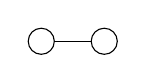
\begin{tikzpicture}[scale=0.8]
\node[circle, draw] (a) at (0,0) {};
\node[circle, draw] (b) at (1,0) {};
\draw (a) -- (b);
    \end{tikzpicture}
    \caption{$G_{1}(\completegraphp{2})$ \\$e=1$, $\mathrm{t}(e)=1$}
    \label{fig:graph_e_1}
\end{subfigure}
\hfill
% ---------- G_2 ----------
\begin{subfigure}{0.18\textwidth}
    \centering
    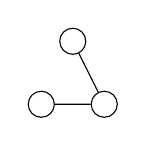
\begin{tikzpicture}[scale=0.8]
\node[circle, draw] (a) at (0,0) {};
\node[circle, draw] (b) at (1,0) {};
\node[circle, draw] (c) at (0.5,1) {};
\draw (a) -- (b) -- (c);
    \end{tikzpicture}
    \caption{$G_{2}$ \\$e=2$, $\mathrm{t}(e)=1$}
     \label{fig:graph_e_2}
\end{subfigure}
\hfill
% ---------- G_3 ----------
\begin{subfigure}{0.18\textwidth}
    \centering
    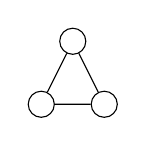
\begin{tikzpicture}[scale=0.8]
\node[circle, draw] (a) at (0,0) {};
\node[circle, draw] (b) at (1,0) {};
\node[circle, draw] (c) at (0.5,1) {};
\draw (a) -- (b) -- (c) -- (a);
    \end{tikzpicture}
    \caption{ $G_{3}(\completegraphp{3})$\\$e=3$, $\mathrm{t}(e)=2$}
     \label{fig:graph_e_3}
\end{subfigure}
\hfill
% ---------- G_4 ----------
\begin{subfigure}{0.18\textwidth}
    \centering
    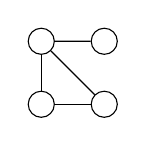
\begin{tikzpicture}[scale=0.8]
\node[circle, draw] (a) at (0,0) {};
\node[circle, draw] (b) at (1,0) {};
\node[circle, draw] (c) at (1,1) {};
\node[circle, draw] (d) at (0,1) {};
\draw (a) -- (b);
\draw (b) -- (d);
\draw (c) -- (d);
\draw (a) -- (d);
    \end{tikzpicture}
    \caption{$G_{4}$\\$e=4$, $\mathrm{t}(e)=2$}
     \label{fig:graph_e_4}
\end{subfigure}
\hfill
% ---------- G_5 ----------
\begin{subfigure}{0.18\textwidth}
    \centering
    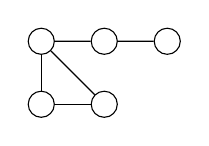
\begin{tikzpicture}[scale=0.8]
\node[circle, draw] (a) at (0,0) {};
\node[circle, draw] (b) at (1,0) {};
\node[circle, draw] (c) at (1,1) {};
\node[circle, draw] (d) at (0,1) {};
\node[circle, draw] (e) at (2,1) {};
\draw (a) -- (b);
\draw (b) -- (d);
\draw (c) -- (d);
\draw (a) -- (d);
\draw (c) -- (e);
    \end{tikzpicture}
    \caption{$G_{5}$\\$e=5$, $\mathrm{t}(e)=1$}
     \label{fig:graph_e_5}
\end{subfigure}

\vspace{0.5cm}

% ========== Row 2: G_6 to G_10 ==========
% ---------- G_6 ----------
\begin{subfigure}{0.18\textwidth}
    \centering
    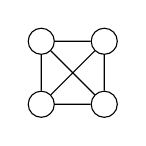
\begin{tikzpicture}[scale=0.8]
\node[circle, draw] (a) at (0,0) {};
\node[circle, draw] (b) at (1,0) {};
\node[circle, draw] (c) at (1,1) {};
\node[circle, draw] (d) at (0,1) {};
\draw (a) -- (b) -- (c) -- (d) -- (a);
\draw (a) -- (c);
\draw (b) -- (d);
    \end{tikzpicture}
    \caption{ $G_{6}(\completegraphp{4})$\\$e=6$, $\mathrm{t}(e)=3$}
     \label{fig:graph_e_6}
\end{subfigure}
\hfill
% ---------- G_7 ----------
\begin{subfigure}{0.18\textwidth}
    \centering
    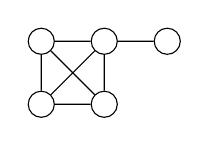
\begin{tikzpicture}[scale=0.8]
\node[circle, draw] (a) at (0,0) {};
\node[circle, draw] (b) at (1,0) {};
\node[circle, draw] (c) at (1,1) {};
\node[circle, draw] (d) at (0,1) {};
\node[circle, draw] (e) at (2,1) {};
\draw (a) -- (b) -- (c) -- (d) -- (a);
\draw (a) -- (c);
\draw (b) -- (d);
\draw (c) -- (e);
    \end{tikzpicture}
    \caption{$G_{7}$\\$e=7$, $\mathrm{t}(e)=3$}
     \label{fig:graph_e_7}
\end{subfigure}
\hfill
% ---------- G_8 ----------
\begin{subfigure}{0.18\textwidth}
    \centering
    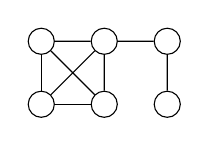
\begin{tikzpicture}[scale=0.8]

        \node[circle, draw] (a) at (0,0) {};
        \node[circle, draw] (b) at (1,0) {};
        \node[circle, draw] (c) at (1,1) {};
        \node[circle, draw] (d) at (0,1) {};

        \node[circle, draw] (e) at (2,1) {};
        \node[circle, draw] (f) at (2,0) {};

        \draw (a) -- (b);
        \draw (a) -- (c);
        \draw (a) -- (d);
        \draw (b) -- (c);
        \draw (b) -- (d);
        \draw (c) -- (d);

        \draw (c) -- (e);
        \draw (e) -- (f);
    \end{tikzpicture}
    \caption{$G_{8}$\\$e=8$, $\mathrm{t}(e)=4$}
     \label{fig:graph_e_8}
\end{subfigure}
\hfill
% ---------- G_9 ----------
\begin{subfigure}{0.18\textwidth}
    \centering
    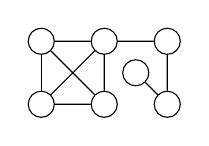
\begin{tikzpicture}[scale=0.8]
\node[circle, draw] (a) at (0,0) {};
\node[circle, draw] (b) at (1,0) {};
\node[circle, draw] (c) at (2,0) {};
\node[circle, draw] (d) at (0,1) {};
\node[circle, draw] (e) at (1,1) {};
\node[circle, draw] (h) at (2,1) {};
\node[circle, draw] (g) at (1.5,0.5) {};
\draw (a) -- (b) -- (d) -- (e);
\draw (c) -- (h) -- (e);
\draw (a) -- (d);
\draw (b) -- (e);
\draw (a) -- (e);
\draw (c) -- (g);
    \end{tikzpicture}
    \caption{$G_{9}$\\$e=9$, $\mathrm{t}(e)=3$}
     \label{fig:graph_e_9}
\end{subfigure}
\hfill
% ---------- G_{10} ----------
\begin{subfigure}{0.18\textwidth}
    \centering
    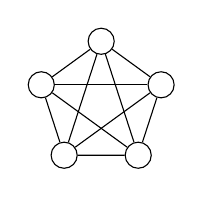
\begin{tikzpicture}[scale=0.8]
\node[circle, draw] (a) at (90:1) {};
\node[circle, draw] (b) at (162:1) {};
\node[circle, draw] (c) at (234:1) {};
\node[circle, draw] (d) at (306:1) {};
\node[circle, draw] (e) at (18:1) {};
\draw (a) -- (b) -- (c) -- (d) -- (e) -- (a);
\draw (a) -- (c);
\draw (a) -- (d);
\draw (b) -- (d);
\draw (b) -- (e);
\draw (c) -- (e);
    \end{tikzpicture}
    \caption{ $G_{10}(\completegraphp{5})$\\$e=10$, $\mathrm{t}(e)=4$}
     \label{fig:graph_e_10}
\end{subfigure}

\vspace{0.5cm}

% ========== Row 3: G_11 to G_15 ==========
% ---------- G_11 ----------
\begin{subfigure}{0.18\textwidth}
    \centering
    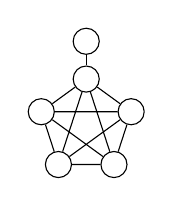
\begin{tikzpicture}[scale=0.6]
        % K5 base nodes in circle
        \node[circle, draw] (v1) at (90:1) {};
        \node[circle, draw] (v2) at (18:1) {};
        \node[circle, draw] (v3) at (306:1) {};
        \node[circle, draw] (v4) at (234:1) {};
        \node[circle, draw] (v5) at (162:1) {};
        
        % K5 edges
        \draw (v1) -- (v2) -- (v3) -- (v4) -- (v5) -- (v1);
        \draw (v1) -- (v3) -- (v5) -- (v2) -- (v4) -- (v1);
        
        % Added vertex and edge
        \node[circle, draw] (v6) at (90:1.8) {};
        \draw (v6) -- (v1);
    \end{tikzpicture}
    \caption{ $G_{11}$\\$e=11$, $\mathrm{t}(e)=4$}
     \label{fig:graph_e_11}
\end{subfigure}
\hfill
% ---------- G_12 ----------
\begin{subfigure}{0.18\textwidth}
    \centering
    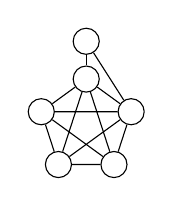
\begin{tikzpicture}[scale=0.6]
        % K5 base nodes in circle
        \node[circle, draw] (v1) at (90:1) {};
        \node[circle, draw] (v2) at (18:1) {};
        \node[circle, draw] (v3) at (306:1) {};
        \node[circle, draw] (v4) at (234:1) {};
        \node[circle, draw] (v5) at (162:1) {};
        
        % K5 edges
        \draw (v1) -- (v2) -- (v3) -- (v4) -- (v5) -- (v1);
        \draw (v1) -- (v3) -- (v5) -- (v2) -- (v4) -- (v1);
        
        % Added vertex and edges
        \node[circle, draw] (v6) at (90:1.8) {};
        \draw (v6) -- (v1);
        \draw (v6) -- (v2);
    \end{tikzpicture}
    \caption{ $G_{12}$\\$e=12$, $\mathrm{t}(e)=4$}
     \label{fig:graph_e_12}
\end{subfigure}
\hfill
% ---------- G_13 ----------
\begin{subfigure}{0.18\textwidth}
    \centering
    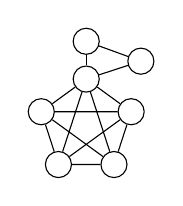
\begin{tikzpicture}[scale=0.6]
        % K5 base nodes in circle
        \node[circle, draw] (v1) at (90:1) {};
        \node[circle, draw] (v2) at (18:1) {};
        \node[circle, draw] (v3) at (306:1) {};
        \node[circle, draw] (v4) at (234:1) {};
        \node[circle, draw] (v5) at (162:1) {};
        
        % K5 edges
        \draw (v1) -- (v2) -- (v3) -- (v4) -- (v5) -- (v1);
        \draw (v1) -- (v3) -- (v5) -- (v2) -- (v4) -- (v1);
        
        % Added vertices and edges
        \node[circle, draw] (v6) at (90:1.8) {};
        \node[circle, draw] (v7) at (50:1.8) {};
        \draw (v6) -- (v1);
        \draw (v7) -- (v1);
        \draw (v6) -- (v7);
    \end{tikzpicture}
    \caption{ $G_{13}$\\$e=13$, $\mathrm{t}(e)=4$}
\end{subfigure}
\hfill
% ---------- G_14 ----------
\begin{subfigure}{0.18\textwidth}
    \centering
    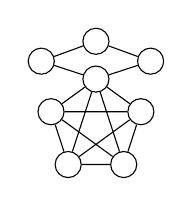
\begin{tikzpicture}[scale=0.6]
        % K5 base nodes in circle
        \node[circle, draw] (v1) at (90:1) {};
        \node[circle, draw] (v2) at (18:1) {};
        \node[circle, draw] (v3) at (306:1) {};
        \node[circle, draw] (v4) at (234:1) {};
        \node[circle, draw] (v5) at (162:1) {};
        
        % K5 edges
        \draw (v1) -- (v2) -- (v3) -- (v4) -- (v5) -- (v1);
        \draw (v1) -- (v3) -- (v5) -- (v2) -- (v4) -- (v1);
        
        % Added vertices forming a square with diagonal connected to v1
        \node[circle, draw] (v6) at (90:1.8) {};
        \node[circle, draw] (v7) at (50:1.8) {};
        \node[circle, draw] (v8) at (130:1.8) {};
        \draw (v7) -- (v1);
        \draw (v8) -- (v1);
        \draw (v6) -- (v7);
        \draw (v8) -- (v6);
    \end{tikzpicture}
    \caption{ $G_{14}$\\$e=14$, $\mathrm{t}(e)=4$}
\end{subfigure}
\hfill
% ---------- G_15 (K6) ----------
\begin{subfigure}{0.18\textwidth}
    \centering
    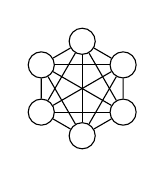
\begin{tikzpicture}[scale=0.6]
        % K6 nodes in circle
        \node[circle, draw] (v1) at (90:1) {};
        \node[circle, draw] (v2) at (30:1) {};
        \node[circle, draw] (v3) at (330:1) {};
        \node[circle, draw] (v4) at (270:1) {};
        \node[circle, draw] (v5) at (210:1) {};
        \node[circle, draw] (v6) at (150:1) {};
        
        % All possible edges for K6 (complete graph)
        \draw (v1) -- (v2);
        \draw (v1) -- (v3);
        \draw (v1) -- (v4);
        \draw (v1) -- (v5);
        \draw (v1) -- (v6);
        \draw (v2) -- (v3);
        \draw (v2) -- (v4);
        \draw (v2) -- (v5);
        \draw (v2) -- (v6);
        \draw (v3) -- (v4);
        \draw (v3) -- (v5);
        \draw (v3) -- (v6);
        \draw (v4) -- (v5);
        \draw (v4) -- (v6);
        \draw (v5) -- (v6);
    \end{tikzpicture}
    \caption{ $G_{15}$ ($\completegraphp{6}$)\\$e=15$, $\mathrm{t}(e)=5$}
\end{subfigure}

\caption{Graphs $G_1$ to $G_{15}$ with increasing edges and maximum treewidth.}
\label{fig:treewidth_table}
\end{figure}

\section{Supplementary Results of Section~\ref{sec:example_hoif}}
\label{app:HOIF}

The following table lists the total number of $V$-statistics and the number of floating-point operations (FLOPs) that need to be computed before and after applying the sparsification trick when the sample size is $10^4$. The rightmost column of Table~\ref{tab:HOIF} also records the value of $M$ defined in Corollary~\ref{cor:U}. 

\begin{table}[htbp]
\centering
\caption{Exact number of floating-point operations (FLOPs), $V$-statistic decompositions, intermediate tensor sizes, 
and the maximum treewidth $M$ across all decomposition graphs 
for HOIF orders from $2$ to $12$, with and without the sparsification trick, where the \Einsum{} ordering is found by applying \opteinsum{} with optimization scheme \texttt{greedy}. Sample size is fixed at $n=10000$.}
\label{tab:HOIF}
\begin{tabular}{cccccc}
\toprule
\textbf{Order ($m$)} & \makecell{\textbf{V-stat terms} \\ \textbf{(Bell number)}} & \makecell{\textbf{V-stat terms} \\ \textbf{(sparsification)}} & \makecell{\textbf{FLOPs} \\ \textbf{(initial)}} & \makecell{\textbf{FLOPs} \\ \textbf{(sparsification)}} & \makecell{$M$} \\
\midrule
2  & 2        & 1        & $2.00020\times10^8$        & $2.00000\times10^8$        & $1$        \\
3  & 5        & 2        & $2.00060\times10^{12}$     & $2.00020\times10^{12}$     & $1$        \\
4  & 15       & 5        & $8.00310\times10^{12}$     & $4.00150\times10^{12}$     & $2$        \\
5  & 52       & 15       & $5.20133\times10^{13}$     & $2.60045\times10^{13}$     & $2$       \\
6  & 203      & 52       & $2.94069\times10^{14}$     & $1.20020\times10^{14}$     & $2$          \\
7  & 877      & 203      & $1.78236\times10^{15}$     & $6.32091\times10^{14}$     & $2$          \\
8  & 4140     & 877      & $2.31054\times10^{17}$     & $2.23430\times10^{17}$     & $3$          \\
9  & 21147    & 4140     & $5.29126\times10^{18}$     & $3.47959\times10^{18}$     & $3$       \\
10 & 115975   & 21147    & $2.07990\times10^{21}$     & $2.04048\times10^{21}$     & $3$        \\
11 & 678570   & 115975   & $5.50026\times10^{22}$     & $3.72144\times10^{22}$     & $4$       \\
12 & 4213597  & 678570   & $1.13401\times10^{24}$     & $6.62181\times10^{23}$     & $4$        \\
\bottomrule
\end{tabular}
\end{table}

We can derive the sharp treewidth bounds presented in Table~\ref{tab:HOIF} using similar techniques to the above in Appendix~\ref{app:treewidtg_table}. For each $m \in \{2, 3, \cdots, 12\}$, the corresponding decomposition signature takes the following form: $\calA_{m} = ((1, 2), \cdots, (m - 1, m))$. Hence by Definition~\ref{def:graph_decomp}, the corresponding decomposition graph $G_{\calA_{m}}$ is the graph with $V(G_{\calA_{m}}) = [m]$, $E(G_{\calA_{m}}) = \{ \{i, i+1\} \}_{i=1}^{m-1}$, whose structure is illustrated in Figure~\ref{fig:hoif_graph_m}.

The result is formally stated in the following observation. 
\begin{observation}
\label{obs:HOIF}    
    For $m = 2,3,\cdots, 12$, let $\calA_{m} = ((1,2),\cdots,(m-1,m))$, and $G_{\calA_m}$ be the corresponding decomposition graph. Similar to Corollary~\ref{cor:U}, $M(m)$ is defined as 
    \begin{align*}
        M(m) \coloneqq \max \{ \treewidthp{G_{\calA_m} /\pi} \mid \pi \in \partitionp{m}^{\calA_m}\}. 
    \end{align*}
    Then the following hold:
    \begin{equation}
    \label{HOIF_M}
    \begin{split}
    M (m) = \left\{ \begin{array}{ll}
    1, & m \in \{2, 3\}, \\
    2, & m \in \{4, 5, 6, 7\}, \\
    3, & m \in \{8, 9, 10\}, \\
    4, & m \in \{11, 12\}.
    \end{array} \right.
    \end{split}
    \end{equation}
\end{observation}

\begin{proof}
Let $\graphset^{\mathsf{HOIF}}_{m} \coloneqq \{ G_{\calA_m} /\pi \mid \pi \in \partitionp{m}^{\calA_m} \}$ then $M(m) \equiv \max \{ \treewidthp{G} \mid G \in \graphset^{\mathsf{HOIF}}_{m} \}$ and it holds that
\begin{equation*}
| E(G) | \leq m-1, \; \forall \, G \in \graphset^{\mathsf{HOIF}}_{m}.
\end{equation*}
A direct application of Observation~\ref{pro:treewidth_table} gives us the following upper bounds: $M(m) \le \mathrm{t}(m-1)$, summarized in Table~\ref{tab:HOIF_upper_bound}. The desired result then follows from a characterization of the lower bound of $M (m)$.

\begin{table}[ht]
    \centering
    \caption{Upper bounds of $M(m)$ for HOIFs: via $M(m) \leq \mathrm{t}(m-1)$. }
    \label{tab:HOIF_upper_bound}
    \begin{tabular}{ccc}
        \toprule
        $m$ & $e$ & $\mathrm{t}(e)$ \\
        \midrule
        2, 3 & 1 & 1 \\
        4, 5, 6 & 3, 4, 5 & 2 \\
        7, 8, 9, 10 & 6, 7, 8, 9 & 3 \\
        11, 12 & 10, 11 & 4 \\
        \bottomrule
    \end{tabular}
\end{table}

We observe that except for $m=7$, the upper bounds match the claimed results in \eqref{HOIF_M}. The lower bounds of $M(m)$ can be obtained by enlisting some concrete examples, which are given in Table~\ref{tab:HOIF_lower_bound}. 

\begin{table}[h]
\centering
\caption{Lowers bound of $M(m)$ for HOIFs: via finding the exemplified graph.}
\label{tab:HOIF_lower_bound}
\begin{tabular}{c c c c}
\toprule
$m$ & $\pi$ & Graph $\graphform{\calA_{m}} /\pi$ & $\treewidthp{\graphform{\calA_{m}} /\pi}$ \\
\midrule
2  & \{\{1\}, \{2\}\} & Figure~\ref{fig:graph_e_1}: $G_1$ & 1 \\
3  & \{\{1\}, \{2\}, \{3\}\} & Figure~\ref{fig:graph_e_2}: $G_2$ & 1 \\
4  & \{\{1, 4\}, \{2\}, \{3\}\} & Figure~\ref{fig:graph_e_3}: $G_3$ & 2 \\
5  & \{\{1, 4\}, \{2\}, \{3\}, \{5\}\} & Figure~\ref{fig:graph_e_4}: $G_4$ & 2 \\
6  & \{\{1, 4\}, \{2\}, \{3\}, \{5\}, \{6\}\} & Figure~\ref{fig:graph_e_5}: $G_5$ & 2 \\
7  & \{\{1, 4\}, \{2\}, \{3\}, \{5\}, \{6\}, \{7\}\} & Figure~\ref{fig:graph_e_6_hoif}: $G_6^{\prime}$ & 2 \\
8  & \{\{1, 4\}, \{2, 6\}, \{3, 7\}, \{5, 8\}\} & Figure~\ref{fig:graph_e_7}: $G_7$ & 3 \\
9  & \{\{1, 4\}, \{2, 6\}, \{3, 7\}, \{5, 8\}, \{9\}\} & Figure~\ref{fig:graph_e_8}: $G_8$ & 3 \\
10 & \{\{1, 4\}, \{2, 6\}, \{3, 7\}, \{5, 8\}, \{9\}, \{10\}\} & Figure~\ref{fig:graph_e_9}: $G_9$ & 3 \\
11 & \{\{1, 6, 11\}, \{2, 9\}, \{3, 7\}, \{4, 10\}, \{5, 8\}\} & Figure~\ref{fig:graph_e_10}: $G_{10}$ & 4 \\
12 & \{\{1, 6, 11\}, \{2, 9\}, \{3, 7\}, \{4, 10\}, \{5, 8\}, \{12\}\} & Figure~\ref{fig:graph_e_11}: $G_{11}$ & 4 \\
\bottomrule
\end{tabular}
\end{table}


\begin{figure}[h!]
    \centering
    \begin{subfigure}{0.45\textwidth}
        \centering
        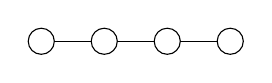
\begin{tikzpicture}[scale=0.8]
            \node[circle, draw] (p1) at (0,0) {};
            \node[circle, draw] (p2) at (1,0) {};   
            \node[circle, draw] (p3) at (2,0) {};
            \node[circle, draw] (p4) at (3,0) {};
            \draw (p1) -- (p2) -- (p3);
            \draw (p3) -- (p4);
        \end{tikzpicture}
        \caption{$\graphform{\calA_m}$ with $m=4$.}
        \label{fig:hoif_graph_m}
    \end{subfigure}
    \hfill
    \begin{subfigure}{0.45\textwidth}
        \centering
        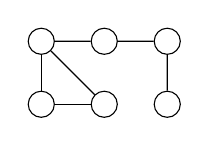
\begin{tikzpicture}[scale=0.8]
            \node[circle, draw] (a) at (0,0) {};
            \node[circle, draw] (b) at (1,0) {};
            \node[circle, draw] (c) at (1,1) {};
            \node[circle, draw] (d) at (0,1) {};
            \node[circle, draw] (e) at (2,1) {};
            \node[circle, draw] (f) at (2,0) {};
            \draw (a) -- (b);
            \draw (b) -- (d);
            \draw (c) -- (d);
            \draw (a) -- (d);
            \draw (c) -- (e);
            \draw (e) -- (f);
        \end{tikzpicture}
        \caption{$G^{\prime}_6:$ the example in Table~\ref{tab:HOIF_lower_bound} when $m=7$.}
        \label{fig:graph_e_6_hoif}
    \end{subfigure}
    \caption{Two decomposition graphs used in Appendix~\ref{app:HOIF}.}
\end{figure}

Combining Table~\ref{tab:HOIF_upper_bound} and Table~\ref{tab:HOIF_lower_bound}, we can conclude that, except for $m = 7$, the upper bound (given in Table~\ref{tab:HOIF_upper_bound}) and the lower bound (given in Table~\ref{tab:HOIF_lower_bound}) of $M (m)$ agree. For $m = 7$, we have $M (7) \in \{2, 3\}$. In the sequel, we will show that $M (7) < 3$ so the claim \eqref{HOIF_M} in Observation~\ref{obs:HOIF} holds.

To this end, we will first establish a lemma (Lemma~\ref{lem:HOIF_table_lem_1}) stating that a simple graph with at most $6$ edges has treewidth $3$ if and only if it is $\completegraphp{4}$ (i.e. the complete graph with $4$ vertices). Then, another lemma (Lemma~\ref{lem:HOIF_table_lem_2}) will show that the set of all quotient graphs of $\graphform{\calA_7}$ does not contain $\completegraphp{4}$. The proof is then complete.
\end{proof}

We first state and prove Lemma~\ref{lem:HOIF_table_lem_1}.
\begin{lemma}
\label{lem:HOIF_table_lem_1}
Recall the definitions of $\mathrm{tt}(n, e)$ and $\graphsetne{n}{e}$ in Lemma~\ref{lem:property_of_tt}. When $1\le e \le  6$, $\mathrm{tt}(n, e) = 3$ if and only if $n = 4, e = 6$, and otherwise $\mathrm{tt}(n, e) < 3$. Moreover, $\graphsetne{4}{6} = \{\completegraphp{4}\}$ up to isomorphism.
\end{lemma}

\begin{proof}
We adopt the same notation as in Lemma~\ref{lem:property_of_tt}.

First, by Observation~\ref{pro:treewidth_table}, we know $\mathrm{t} (e) < 3$ when $1 \le e \le 5$, and $\mathrm{t}(6) = 3$. Thus we only need to consider the case $e = 6$. Note that the support set of $\graphsetne{n}{6}$ is $\mathrm{n}(6) = \{4,5,\dots,12\}$.
    
For $n = 4$, we have $\binom{4}{2} = 6$, and by Property~4 in Lemma~\ref{lem:property_of_tt}, $\mathrm{tt}(4, 6) = 3$ directly follows.  
    
For any $n \in \mathrm{n}(6) \setminus \{4\}$, we have $1 \le \frac{2 \cdot 6}{n} < 3$.  Therefore, $\mathrm{tt}(n, 6) \le \max\{ 2, \mathrm{t}(5) \} < 3$. This proves the first claim.
    
For the second claim, note that any simple graph with $4$ vertices can have at most $\binom{4}{2} = 6$ edges, and the only such graph (up to isomorphism) is $\completegraphp{4}$. 
\end{proof}

Lastly, we state and prove Lemma~\ref{lem:HOIF_table_lem_2}.

\begin{lemma}
\label{lem:HOIF_table_lem_2}
Let $\graphform{\calA_7}$ be the decomposition graph of decomposition signature $\calA_7 = ((i,i+1))_{i=1}^6$. Then no quotient graph of $\graphform{\calA_7}$ is $\completegraphp{4}$ or contains $\completegraphp{4}$ as a subgraph.
\end{lemma}

\begin{proof}
Consider a partition $\pi = \{Q_1, Q_2, \dots, Q_K\} \in \partitionp{7}$ of the vertex set of $\graphform{\calA_7}$, as defined in Definition~\ref{def:quotient_graph}. 
The quotient graph $\graphform{\calA_7} / \pi$ has $|\pi| = K \le 7$ vertices, with each vertex corresponding to a subset $Q_k$ for $k \in [K]$ of the partition $\pi$. An edge exists between $Q_i$ and $Q_j$ ($i \neq j$) in the quotient graph if and only if there is at least one edge in $\graphform{\calA_7}$ connecting a vertex in $Q_i$ to a vertex in $Q_j$.

We observe that $|\edgesp{\graphform{\calA_7} / \pi}| \le |\edgesp{\graphform{\calA_7}}| = 6$ for all $\pi \in \partitionp{7}$, and the inequality is strict whenever any subset $Q_k$ contains adjacent vertices in $\graphform{\calA_7}$.

Since $|\edges(\graphform{\calA_7})| = 6$ and $|\edges(\completegraphp{4})| = \binom{4}{2} = 6$, no quotient graph of $\graphform{\calA_7}$ can contain $\completegraphp{4}$ as a proper subgraph (i.e. a subgraph that is not the original graph). 
Therefore, it suffices to consider the case where $\completegraphp{4}$ is isomorphic to a quotient graph of $\graphform{\calA_7}$. 
For simplicity, we write ``$=$'' to denote graph isomorphism.

Suppose that there exists a partition $\pi^{*} = \{ Q_1, Q_2, Q_3, Q_4 \} \in \Pi_7$ such that $\graphform{\calA_7} / \pi^{*} = \completegraphp{4}$. 
Then, $\pi^{*}$ must satisfy the following conditions:

\begin{enumerate}
    \item No subset $Q_i$ contains adjacent numbers, i.e., $(k, k+1)$ for $k \in \{1,2,\dots,6\}$ and $i \in [4]$;
    \item For any $i \neq j$, there exist $k \in Q_i$ and $k' \in Q_j$ such that $|k - k'| = 1$.
\end{enumerate}

The first condition ensures that $|\edgesp{\graphform{\calA_7} / \pi}| = 6$. 
The second condition ensures that every pair of subsets is connected by at least one edge in the quotient graph. 
Since $\graphform{\calA_7}$ has only $6$ edges, each edge must correspond uniquely to a distinct pair of subsets, covering all $6$ edges of $\completegraphp{4}$.

Define a map $c: [7] \to [4]$ by
\begin{equation*}
    c(k) = i \quad \text{for all } k \in Q_i.
\end{equation*}
By above analysis, all 6 edges in $\graphform{\calA_7} / \pi^*$ must be 
\begin{equation*}
\{ Q_{c(1)}, Q_{c(2)} \}, \ 
\{ Q_{c(2)}, Q_{c(3)} \}, \ 
\{ Q_{c(3)}, Q_{c(4)} \}, \ 
\{ Q_{c(4)}, Q_{c(5)} \}, \ 
\{ Q_{c(5)}, Q_{c(6)} \}, \ 
\{ Q_{c(6)}, Q_{c(7)} \},
\end{equation*}

which forms an Euler trail (i.e., a sequence of edges in which consecutive edges share a common endpoint, visiting every edge of the graph exactly once without repetition.) in the quotient graph $\graphform{\calA_7} / \pi^* = \completegraphp{4}$.

However, by Corollary~4.1 in \citet{bondy1976graph},  
a connected undirected graph admits an Euler trail if and only if it has exactly $0$ or $2$ vertices of odd degree.  
Since $\completegraphp{4}$ has $4$ vertices, each of degree $3$, all vertices have odd degrees, and thus no Euler trail exists.  
This contradiction shows that no partition $\pi^*$ can produce $\completegraphp{4}$ as a quotient graph of $\graphform{\calA_7}$.
\end{proof}

% \section{Illustration of the \Einsum{} Operation via Examples}
% \label{app:contraction ordering}

% To further illustrate our proposed algorithm implemented in \package{}, we use several examples to demonstrate how the \Einsum{} operation is actually executed in practice. There are two objectives that we hope to accomplish: (1) visualizing the \Einsum{} operation further facilitates understanding; (2) it motivates more heuristic algorithms to be developed to further accelerate the \Einsum{} operation. 

% \section{Implementation of the new package \package{}}

% \Lin{we should probably allow others to input only $\calH$, $\calA$, and $\bm{X}$ and directly give users the output, just like what \citet{lee2023ananke} did.}



\section{Supplementary Results of Section~\ref{sec:example_motif}}
\label{app:motifs}

In this section, we first present the $U$-statistic representations for all 3-vertex and 4-vertex motifs mentioned in Section~\ref{sec:example_motif}. Letting $B \equiv 1 - A$, the corresponding $U$-statistics for motif counts for specific $3$-vertex motifs and $4$-vertex motifs (see Figure~\ref{fig:motif-3-4} for which motifs $\sfr_1$ to $\sfr_8$ encode) read as follows:
\begin{align*}
\motifrg{\sfr_1}{G} & = \frac{1}{2} \sum_{ \bar{i}_{3} \in \perm{n,3}}  A_{i_1, i_2} A_{i_2, i_3}  B_{i_3, i_1}, \\ \motifrg{\sfr_2}{G} & = \frac{1}{6} \sum_{ \bar{i}_{3} \in \perm{n,3}}  A_{i_1, i_2} A_{i_2, i_3} A_{i_3, i_1}, \\
\motifrg{\sfr_3}{G} & = \frac{1}{6} \sum_{ \bar{i}_{4} \in \perm{n,4}}  A_{i_1, i_2} A_{i_1, i_3} A_{i_1, i_4} B_{i_2, i_3} B_{i_2, i_4} B_{i_3, i_4}, \\ 
\motifrg{\sfr_4}{G} & = \frac{1}{2} \sum_{ \bar{i}_{4} \in \perm{n,4}}  A_{i_1, i_2} B_{i_1, i_3} B_{i_1, i_4} A_{i_2, i_3} B_{i_2, i_4} A_{i_3, i_4}, \\ 
\motifrg{\sfr_5}{G} & = \frac{1}{2} \sum_{ \bar{i}_{4} \in \perm{n,4}}  A_{i_1, i_2} A_{i_1, i_3} B_{i_1, i_4} A_{i_2, i_3} B_{i_2, i_4} A_{i_3, i_4}, \\ 
\motifrg{\sfr_6}{G} & = \frac{1}{8} \sum_{ \bar{i}_{4} \in \perm{n,4}}  A_{i_1, i_2} B_{i_1, i_3} A_{i_1, i_4} A_{i_2, i_3} B_{i_2, i_4} A_{i_3, i_4}, \\ 
\motifrg{\sfr_7}{G} & = \frac{1}{4} \sum_{ \bar{i}_{4} \in \perm{n,4}}  A_{i_1, i_2} A_{i_1, i_3} A_{i_1, i_4} A_{i_2, i_3} A_{i_2, i_4} B_{i_3, i_4}, \\ 
\motifrg{\sfr_8}{G} & = \frac{1}{24} \sum_{ \bar{i}_{4} \in \perm{n,4}}  A_{i_1, i_2} A_{i_1, i_3} A_{i_1, i_4} A_{i_2, i_3} A_{i_2, i_4} A_{i_3, i_4}.
\end{align*}


\begin{figure}[ht]
    \centering

    \begin{subfigure}{0.22\textwidth}
        \centering
        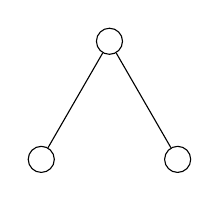
\begin{tikzpicture}
            \node[circle,draw](a) at (0,1) {};
            \node[circle,draw](b) at (-0.866,-0.5) {};
            \node[circle,draw](c) at (0.866,-0.5) {};
            \draw (a) -- (b);
            \draw (a) -- (c);
        \end{tikzpicture}
        \caption{$\sfr_1$: V-shape}
    \end{subfigure}
    \hfill
    \begin{subfigure}{0.22\textwidth}
        \centering
        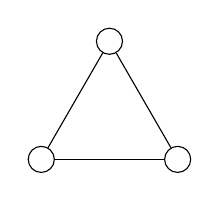
\begin{tikzpicture}
            \node[circle,draw](a) at (0,1) {};
            \node[circle,draw](b) at (-0.866,-0.5) {};
            \node[circle,draw](c) at (0.866,-0.5) {};
            \draw (a) -- (b);
            \draw (a) -- (c);
            \draw (b) -- (c);
        \end{tikzpicture}
        \caption{$\sfr_2$: Triangle}
    \end{subfigure}
    \hfill
    \begin{subfigure}{0.22\textwidth}
        \centering
        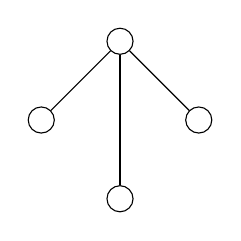
\begin{tikzpicture}
            \node[circle,draw](a) at (0,1) {};
            \node[circle,draw](b) at (-1,0) {};
            \node[circle,draw](c) at (1,0) {};
            \node[circle,draw](d) at (0,-1) {};
            \draw (a) -- (b);
            \draw (a) -- (c);
            \draw (a) -- (d);
        \end{tikzpicture}
        \caption{$\sfr_3$ : 3-star}
    \end{subfigure}
    \hfill
    \begin{subfigure}{0.22\textwidth}
        \centering
        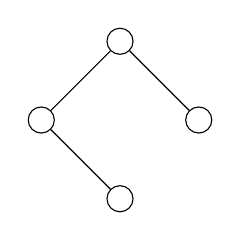
\begin{tikzpicture}
            \node[circle,draw](a) at (0,1) {};
            \node[circle,draw](b) at (-1,0) {};
            \node[circle,draw](c) at (1,0) {};
            \node[circle,draw](d) at (0,-1) {};
            \draw (a) -- (b);
            \draw (a) -- (c);
            \draw (b) -- (d);
        \end{tikzpicture}
        \caption{$\sfr_4$ : Fork}
    \end{subfigure}

    \vspace{1em}

    \begin{subfigure}{0.22\textwidth}
        \centering
        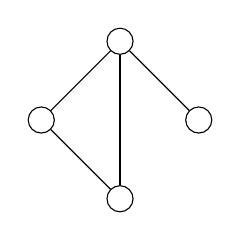
\begin{tikzpicture}
            \node[circle,draw](a) at (0,1) {};
            \node[circle,draw](b) at (-1,0) {};
            \node[circle,draw](c) at (1,0) {};
            \node[circle,draw](d) at (0,-1) {};
            \draw (a) -- (b);
            \draw (a) -- (c);
            \draw (a) -- (d);
            \draw (b) -- (d);
        \end{tikzpicture}
        \caption{$\sfr_5$ : Tailed triangle}
    \end{subfigure}
    \hfill
    \begin{subfigure}{0.22\textwidth}
        \centering
        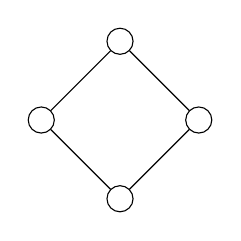
\begin{tikzpicture}
            \node[circle,draw](a) at (0,1) {};
            \node[circle,draw](b) at (-1,0) {};
            \node[circle,draw](c) at (1,0) {};
            \node[circle,draw](d) at (0,-1) {};
            \draw (a) -- (b);
            \draw (a) -- (c);
            \draw (b) -- (d);
            \draw (c) -- (d);
        \end{tikzpicture}
        \caption{$\sfr_6$: Square}
    \end{subfigure}
    \hfill
    \begin{subfigure}{0.22\textwidth}
        \centering
        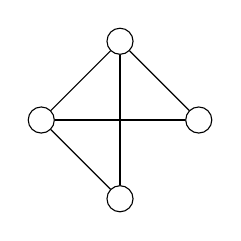
\begin{tikzpicture}
            \node[circle,draw](a) at (0,1) {};
            \node[circle,draw](b) at (-1,0) {};
            \node[circle,draw](c) at (1,0) {};
            \node[circle,draw](d) at (0,-1) {};
            \draw (a) -- (b);
            \draw (a) -- (c);
            \draw (a) -- (d);
            \draw (b) -- (c);
            \draw (b) -- (d);
        \end{tikzpicture}
        \caption{$\sfr_7$: House}
    \end{subfigure}
    \hfill
    \begin{subfigure}{0.22\textwidth}
        \centering
        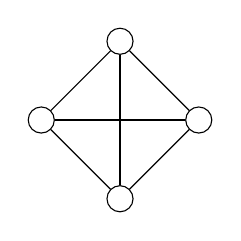
\begin{tikzpicture}
            \node[circle,draw](a) at (0,1) {};
            \node[circle,draw](b) at (-1,0) {};
            \node[circle,draw](c) at (1,0) {};
            \node[circle,draw](d) at (0,-1) {};
            \draw (a) -- (b);
            \draw (a) -- (c);
            \draw (a) -- (d);
            \draw (b) -- (c);
            \draw (b) -- (d);
            \draw (c) -- (d);
        \end{tikzpicture}
        \caption{$\sfr_8$ : 4-clique}
    \end{subfigure}

    \caption{All non-degenerate isomorphism classes of 3-vertex and 4-vertex simple undirected graphs.}
    \label{fig:motif-3-4}
\end{figure}

Therefore, motif counts for $m$-vertex motifs naturally correspond to a complete decomposition signature $\calA_{\mathsf{Motif},m} = ((s,t))_{1 \le s < t \le m}$, where the associated decomposition graph $\graphform{\calA_{\mathsf{Motif},m}}$ is the complete graph $\completegraphp{m}$. 
This structure has two important implications. 

First, by leveraging our sparsification technique (Lemma~\ref{lem:sparsification_trick} and Remark~\ref{eq:quotient_set}), the computation reduces to a single dominant term, i.e.,
\begin{align*}
\partition_m^{\calA_{\mathsf{Motif},m}} 
= \{ \pi_m \}, 
\quad \text{where } 
\pi_m \coloneqq \big\{ \{1\}, \{2\}, \ldots, \{m\} \big\}.
\end{align*}

Second, this also reveals a fundamental limitation. 
Even after sparsification, the resulting term still induces the same complete decomposition structure,
\begin{align*}
\graphform{\calA_{\mathsf{Motif},m}} / \pi_m 
= \completegraphp{m},
\end{align*}
and therefore the computational complexity of exact motif counting cannot be reduced below $\less(n^m)$ within our framework.

We next present the experimental results for 4-vertex motif counting and GPU-based triangle counting, which are summarized in Table~\ref{tab:motif_counts_4} and Table~\ref{tab:triangle_counting_gpu}, respectively. The overall message is quite similar to that in Table~\ref{tab:motif_counts_3} presented in Section~\ref{sec:example_motif}.

\begin{table}[h!]
\centering
\caption{
Runtime comparison of exact all $4$-vertex motif counts using \package{}, \peregrine{} and \igraph{} on Erd\H{o}s--R\'enyi graphs $G(n, p)$ with $n = 2000$. 
Experiments were run on Intel Xeon Scalable Cascade Lake 6248 CPUs (2.5GHz, 40 total cores) with memory of 192 GB.
``OOT'' denotes instances that exceeded the time limit of 3600 seconds.
}
\label{tab:motif_counts_4}
\begin{tabular}{cccc}
\toprule
\makecell{\textbf{Edge} \\ \textbf{Prob.} $p$} & \makecell{\textbf{\package{}} \\ \textbf{Time (s)}} & \makecell{\textbf{\peregrine{}} \\ \textbf{Time (s)}} & \makecell{\textbf{\igraph{}} \\ \textbf{Time (s)}} \\
\midrule
0.0005 & 3.8413 & 0.1024 & 0.0752 \\
0.0010 & 18.7463 & 0.1141 & 0.0873 \\
0.0050 & 41.0730 & 0.1132 & 0.2645 \\
0.0100 & 40.7701 & 0.1116 & 1.7099 \\
0.0500 & 41.5188 & 0.2079 & 610.0180 \\
0.1000 & 40.5648 & 0.8243 & OOT \\
0.2000 & 41.2671 & 5.8045 & OOT \\
0.4000 & 43.3735 & 48.7363 & OOT \\
0.6000 & 39.6022 & 159.4699 & OOT \\
0.8000 & 40.6578 & 292.4395 & OOT \\
\bottomrule
\end{tabular}
\end{table}

\begin{table}[htbp]
\centering
\caption{Runtime comparison of exact triangle counting  using \package{} and \cugraph{} on Erd\H{o}s--R\'enyi graphs $G(n, p)$ with $n = 10000$. Experiments were run on a single GPU (NVIDIA RTX 4090, 24GB) ``OOM" indicates out-of-memory.}
\label{tab:triangle_counting_gpu}
\begin{tabular}{ccc}
\toprule
\makecell{\textbf{Edge} \\ \textbf{Prob.} $p$} & 
\makecell{\textbf{\package{}} \\ \textbf{Time (s)}} & 
\makecell{\textbf{\cugraph{}} \\ \textbf{Time (s)}} \\
\midrule
0.001 & 2.8014 & 0.1536 \\
0.005 & 2.9564 & 0.5664 \\
0.010 & 3.3363 & 1.0379 \\
0.020 & 3.7830 & 1.9797 \\
0.050 & 5.0856 & 4.9804 \\
0.080 & 6.3764 & 8.1346 \\
0.100 & 7.2829 & 10.3661 \\
0.150 & 9.6873 & 15.3828 \\
0.200 & 11.7283 & OOM \\
0.800 & 37.6880 & OOM \\
\bottomrule
\end{tabular}
\end{table}

\putbib[Master.bib]

\end{bibunit}

\end{document}
